\documentclass{article}

\newcommand{\AsAnAside}{\footnotesize}
\newcommand{\code}[1]{{\tt#1}}

\newcommand{\FlashOfTheFuture}{ExaFLASH\xspace}

\newcommand{\ie}{\textit{i.e.}}   % use always with comma following: \ie,
\newcommand{\etc}{etc.\xspace}  % or: {\emph{etc.}\xspace}
\newcommand{\eg}{\textit{e.g.}}   % use always with comma following: \eg,
\newcommand{\N}                 {{\mathbb N}}
\newcommand{\Z}                 {{\mathbb Z}}
\newcommand{\Q}                 {{\mathbb Q}}
\newcommand{\R}                 {{\mathbb R}}
\newcommand{\C}                 {{\mathbb C}}
\newcommand{\F}                 {{\mathbb F}}

\newcommand{\TeamStarting}      {\textsc{TeamStarting}}
\newcommand{\TeamIdle}          {\textsc{TeamIdle}}
\newcommand{\TeamRunningOpen}   {\textsc{TeamRunningOpen}}
\newcommand{\TeamRunningClosed} {\textsc{TeamRunningClosed}}
\newcommand{\TeamRunningNoMoreWork} {\textsc{TeamRunningNoMoreWork}}
\newcommand{\TeamTerminating}   {\textsc{TeamTerminating}}

\newcommand{\ThreadStarting}    {\textsc{ThreadStarting}}
\newcommand{\ThreadIdle}        {\textsc{ThreadIdle}}
\newcommand{\ThreadComputing}   {\textsc{ThreadComputing}}
\newcommand{\ThreadWaiting}     {\textsc{ThreadWaiting}}
\newcommand{\ThreadTerminating} {\textsc{ThreadTerminating}}

\newcommand{\spelledoutOR}   {orchestration runtime\xspace}
\newcommand{\spelledoutOS}   {orchestration system\xspace}

\newcommand{\shortOR}   {OR\xspace}
\newcommand{\shortOS}   {OS\xspace}

\newcommand{\OR}        {\shortOR}
\newcommand{\OS}        {\shortOS}

\newcommand{\taskroutine}        {task routine\xspace}
\newcommand{\taskroutines}       {task routines\xspace}
\newcommand{\Taskroutines}       {Task routines\xspace}
\newcommand{\actionroutine}        {action routine\xspace}       %fka task routine
\newcommand{\actionroutines}       {action routines\xspace}
\newcommand{\job}                {\textbf{job}\xspace}  % == \taskroutine execution ?
\newcommand{\jobs}               {\textbf{jobs}\xspace}  % == \taskroutine executions ?




% No automatic indenting
\setlength\parindent{0pt}

% Set spacing between items in itemize/enumerate
\setlist{itemsep=1pt}

\DefineVerbatimEnvironment{codeseg}{Verbatim}{frame=none}
\DefineVerbatimEnvironment{fcodeseg}{Verbatim}{frame=single,framerule=1pt,framesep=5mm}
\DefineVerbatimEnvironment{fncodeseg}{Verbatim}{frame=single,framerule=1pt,framesep=5mm,numbers=left}
\newenvironment{shrink}{%
\begin{center}
\begin{minipage}{0.8\textwidth}}
{\end{minipage}\end{center}}


\title{\FlashOfTheFuture Orchestration System Design}


\begin{document}
\lstset{language=[08]Fortran,frame=single,numbers=left,numberstyle=\scriptsize,basicstyle=\small,
captionpos=b}

% Setup numbered/referentiable environment for requirements
\theoremstyle{definition} % No italics or spaces
\newtheorem{req}{Req}[section]
\newtheorem{spec}{Spec}[section]

\maketitle

\tableofcontents

%%%%%----- ORCHESTRATION SYSTEM EXECUTIVE SUMMARY -----%%%%%
\section{Executive Summary}


This document is intended to be a static snapshot of the \FlashOfTheFuture development
team's understanding of the design and requirements associated with the
Orchestration System that is under development for inclusion in \FlashOfTheFuture.  This
document has been informed by discussions within the group and with
collaborators as well as through some prototyping of the Orchestration Runtime
in \FlashOfTheFuture with the \texttt{simpleUnsplit} Hydro implementation.  However, as a
static document, the contents here will likely not be updated as our
understanding of the design of this system improves with implementation of the
system.\\

The \textbf{orchestration system} is a performance portability system that will
allow \FlashOfTheFuture to run in CPU-only mode or to make good, efficient use of resources
when run on heterogeneous platforms on which the notion of host-to-device
offloading exists. The orchestration system is comprised of
three offline components and one runtime component, namely
\begin{enumerate}
\item{an offline \textbf{\spelledoutKGC} (henceforth: \textbf{\shortKGC}),}
\item{an offline \textbf{task scheduler} (henceforth: \textbf{\shortTS}),}
\item{an offline \textbf{code generator} (henceforth: \textbf{\shortCG}), and}
\item{an \textbf{orchestration runtime} (henceforth: \textbf{\shortOR}).}
\end{enumerate}

The \OR is needed to expose the hierarchy of parallelism of a
given platform's hardware; the collection of offline tools, to adapt the
software to the interface exposed by the \OR so that the software can take advantage of the exposed
parallelism.  The division of labor between multiple tools is made not only to
achieve good encapsulation and modularity, but also to ensure that no single
tool is too complex or requires too much intelligence.  Refer to
Table~\ref{tab:ParallelHierarchy} for a detailed view of the aforementioned
hierarchy.\\

Our design is forward-looking in the sense that we hope our
design will not preclude running on future heterogeneous platforms in which
multiple distinct devices including the host might exist in the same chip
package (higher NUMA complexity) or in which multiple distinct devices including
the host might share the same physical memory package (altering the role of data
transport in a single simulation).  Specifically, our three-levels of
future-proofing consider that the design must allow for
\begin{itemize}
\item{One host + many accelerators (offloading),}
\item{tighter coupling between host \& host devices
(physically-unified memory / GPU and CPU have the same memory) --- memory
barriers to manage resource access dependencies.  \Jared{Tighter than what?} NUMA effects (e.g. GPU and CPU
on same chip) would require that user can dictate mapping of tasks onto HW.
Same memory could mean that data movements become unnecessary.  This last point
seems hard.}
\item{Runtime adaptiveness/forecasting --- this is the interface between the
\OR and the offline tools --- we have the \OR public
interface that dictates how different computational actions can be bundled
together for execution on the underlying hardware in one single call to the
runtime and on the other side a graph of actions to be applied that
must be expressed as bundled actions for execution by the \OR.}
\end{itemize}

We emphasize that not only should the design/implementation allow for us to
account for future developments, but also adjusting the
design/implementation should be scalable such that updating the software to use
new or different hardware features should be easy and result in maintainable
code.

\begin{table}[!t]
\label{tab:ParallelHierarchy}
\caption{The hierarchy of parallelism that the Orchestration System design
should expose and capitalize on.  The table is ordered from coarsest parallelism
(top) to finest.  Refer to Section~\ref{sec:Definitions} for definitions of
terms that appear in the table and Section~\ref{sec:Runtime} for more
information regarding Thread Teams.  The HW Scope column indicates the coarsest
level of granularity of a platform's hardware at which the parallelization is
implemented; SW Scope, the coarsest element of the SW architecture at which the
parallelization is implemented.

}

\begin{center}

\begin{tabular}{|p{1.35in}|c|c|c|p{2.25in}|}
\hline
Title & Parallelism & HW Scope & SW Scope & Description\\
\hline
\hline
MPI                              & Data Parallel & Machine & Domain    & Domain decomposition into blocks\\
\hline
Block Iterator                   & Asynchrony    & Machine & Time step & Overlay guardcell fill communication with computation\\
\hline
Task Routine Bundles with
                     concurrency & Task Parallel & Node    & Time step & Run
                     independent \ULtaskregs concurrently to maximize usage of
                     all HW resources in nodes\\
\hline
Task Routine Bundles with
                  work splitting & Data Parallel & Node    & Time step & Use different devices to apply a single \ULtaskreg to assigned blocks\\
\hline
Thread Teams                     & Data Parallel & Node    &Task Region& Apply a single task routine to assigned blocks using host and optionally accelerators\\
\hline
Device Kernels                   & Data Parallel & Device  & Kernel    & Oversubscribe device with kernels to hide latencies\\
\hline
Device HW                        & Data Parallel & Device  & Comp.     & Schedule individual computations across processing units in device\\
\hline
\end{tabular}

\end{center}
\end{table}

\begin{figure}[!hp]
\begin{center}
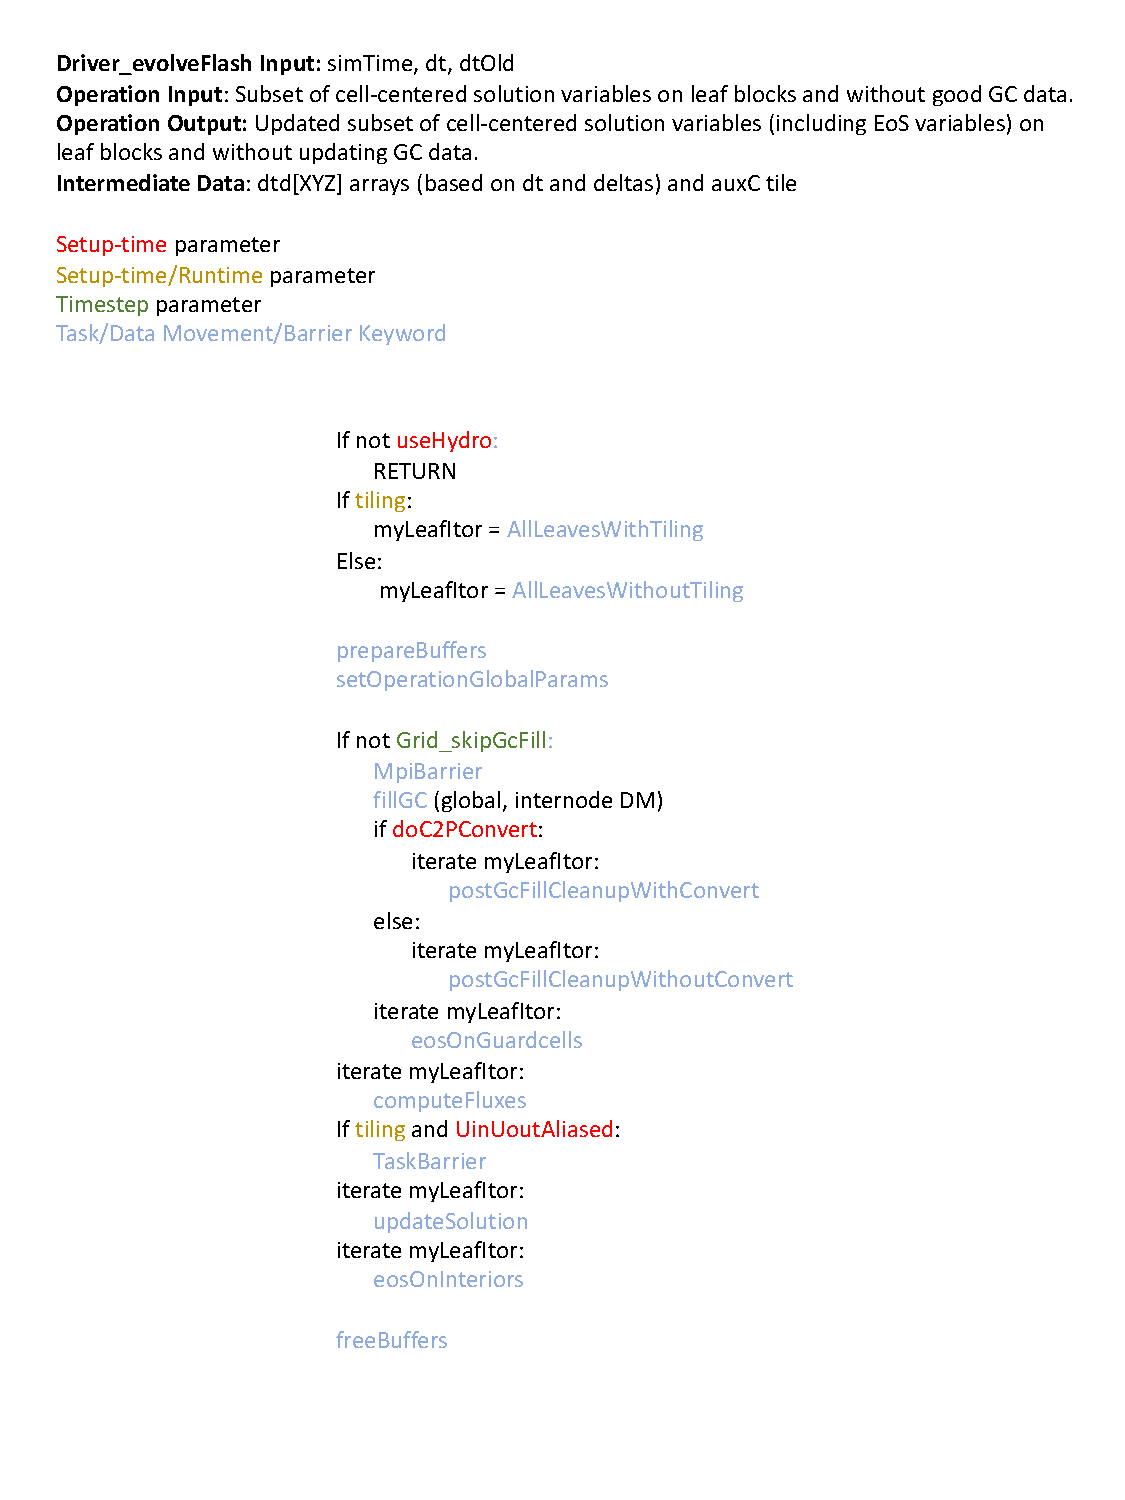
\includegraphics[height=8.0in]{simpleUnsplitAlgo.pdf}
\caption[]{An example of a python-like, high-level representation of the
\texttt{simpleUnsplit} operation for advancing the hydrodynamics solution by one
time step.  The words in light blue indicate key values that index into a
dictionary of operation-level action regions (\OLARs), data movement regions, and barriers.}
\label{fig:simpleUnsplitAlgo}
\end{center}
\end{figure}

\begin{figure}[!hp]
\begin{center}
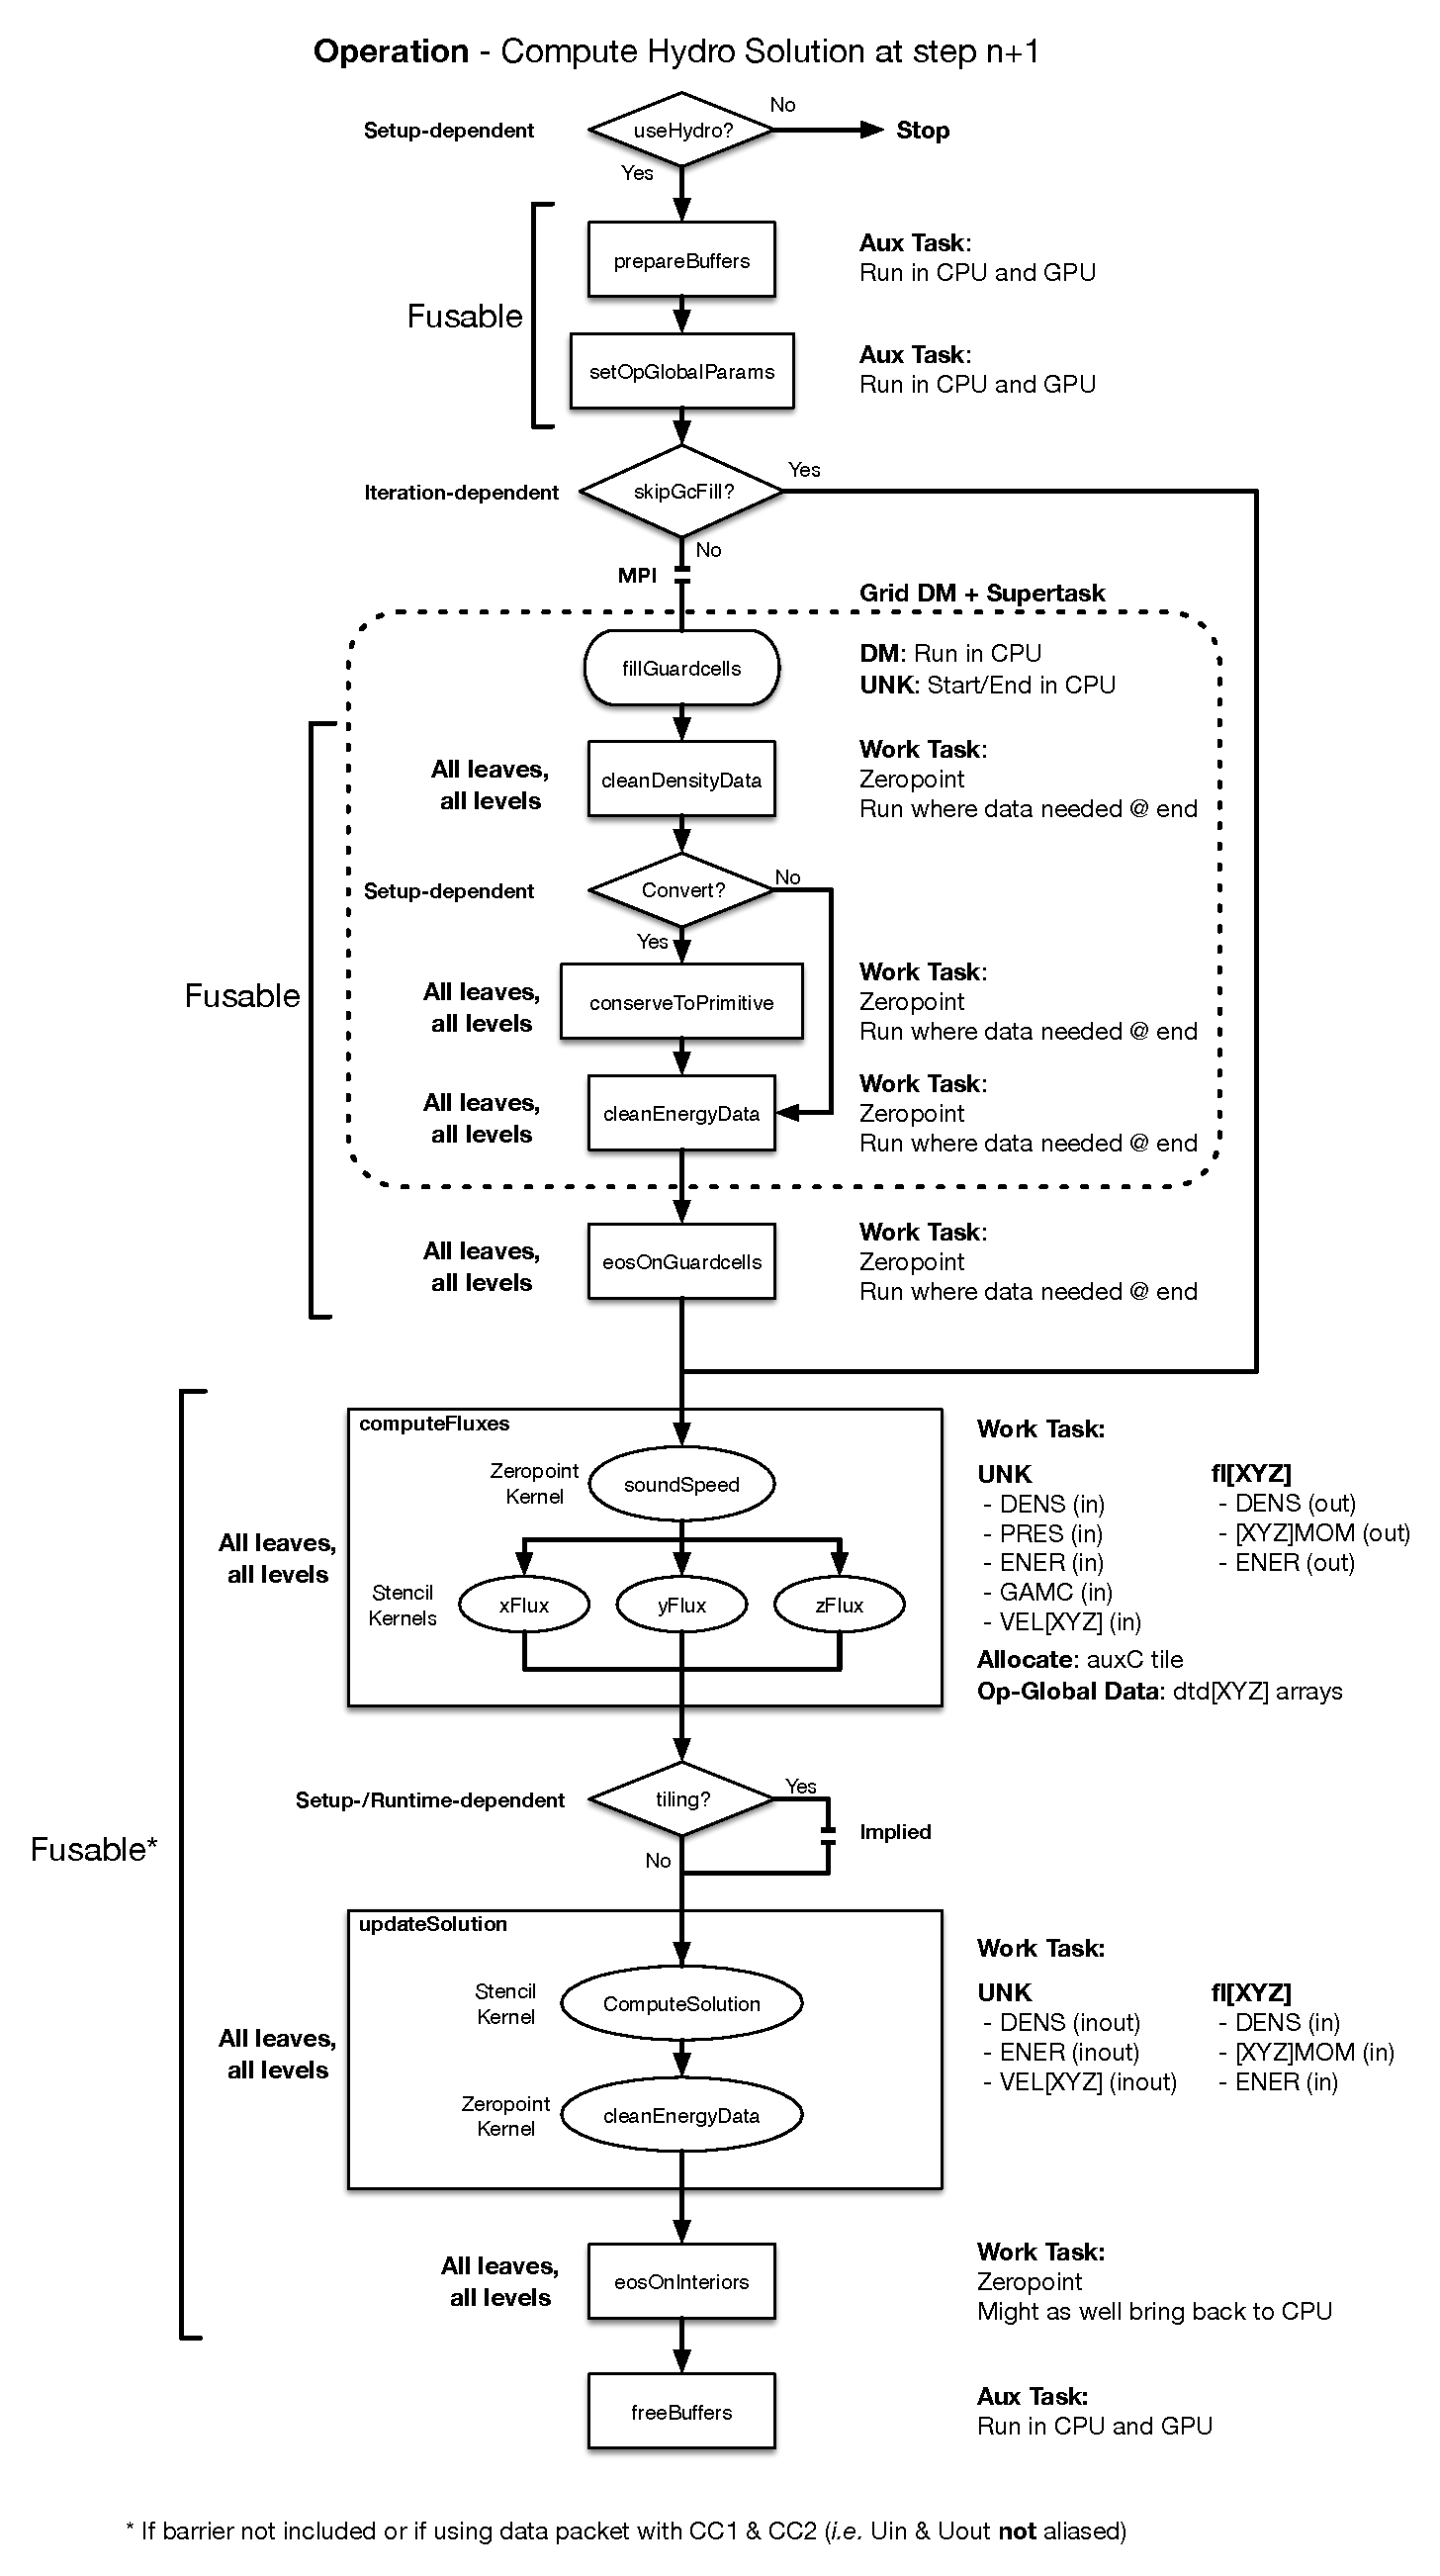
\includegraphics[height=8.5in]{simpleUnsplitFlow.pdf}
\caption[]{Graphic representation of the information that might be contained in a decorated kernel graph,
for the
\texttt{simpleUnsplit} operation for advancing the hydrodynamics solution by one time step to $t_{n+1}$
in solution advance phase number $n+1$.
This demonstrates what the \KGC may produce from the input in Figure~\ref{fig:simpleUnsplitAlgo}.}
\label{fig:simpleUnsplitKernelGraph}
\end{center}
\end{figure}

%%%%%----- ORCHESTRATION SYSTEM DEFINITIONS & OVERVIEW -----%%%%%
\newpage
\section{Orchestration System General Design}
The section introduces terms and concepts that will be used throughout the
document.  Its purpose is to present the reader with a high-level overview of
the orchestration system design.  The contents of this section are non-technical
and should \textbf{not} be used to generate a design nor inform an
implementation of the design.  Refer to later sections containing requirements
and technical specifications to find technical details that can be used for such
purposes.\\

\subsection{Approaching ExaFLASH}

Users OF ExaFLASH will write their algorithms in a source code form
that combines fragments of source code in a traditional programming language (currently: Fortran)
with structural and descriptive features. The Orchestration system takes
sections of algorithms written this way, analyzes and transforms them,
and by combining them with additional initialization, skeleton, and infrastructure code
generates executable code that efficiently implements a simulation
that consists of successive application of such algorithms. Users do not need to know
the details of the local patching or tiling used by the Orchestration System and are free to focus on
research and goals. \\



\subsection{Fundamental Concepts and Definitions}
Note that the following terms are used with special meaning. Additional definitions will be given
\textit{passim} after the overview.


\subsubsection{Conceptual Terminology}
This subsection serves for background and motivation.
It introduces, in a generic way, several concepts that will
reappear with more concrete definitions in later sections;
in particular, several of the concepts mentioned here have
corresponding concrete meaning in the \PUD view of code (\ref{sec:PUDCodeTerminology}), on the one hand,
and in the \OR view of code (\ref{sec:ORCodeTerminology}) on the other.
The reader may safely skip over this subsection.

\\

\begin{itemize}
\item \textbf{activity}.
An \textbf{activity} is ``something to do'', considered separately from any
specific instance of doing it.
We will often name an activity with a
gerund phrase like \emph{smoothing} or \emph{computing the pressure}.

For this definition, activities
are ultimately applicable in a discrete representation.
The continuous
world of real multivariate functions and operators is outside
of our scope here, even though it will probably be in the back of our minds.

Specifying an activity
means saying \textit{what to do}; without specifying the object (\textit{to what?}) or domain region \textit{where?}.

Activities can have different degrees of specificity.
Examples:
\begin{enumerate}
\item smoothing
\item smoothing density
\item recomputing specific energy from velocity components
\item recomputing specific energy from velocity components on a subdomain
\item recomputing specific energy from velocity components on a tile
\item recomputing specific energy from velocity components on a set of tiles
\item computing fluxes
\end{enumerate}
Activities 4--6 show, we consider an elaboration of the object to which
an activity applies as a legitimate degree of specificity.

An activity, when applied to specific
objects or \domregions, yields a meaningful task.


\item \textbf{action}.
An \textbf{action} is an activity with specificity about the object.
Specifying an action
means saying \textit{what to do} on \textit{what type of objects(s)}.

An action is comparable to a mathematical operator. An operator
is a prescription of what to do, but does not imply a
specific instance of an object. It does
indicate the type(s) of object(s) for the action.

\item \textbf{task}.
A \textbf{task} is one instance of applying an action to one data item.
A task
means saying \textit{Do this on this data item once}.

 \textbf{Task} is essentially a run-time concept:
multiple applications of the same action are considered
different tasks, whether or not they apply to the same data item each time.

\item \textbf{job}.
A \textbf{job} is one instance of applying an action to a collection of data items.
A job
means saying \textit{Do this on these data items once}.

\textbf{Job} is essentially a run-time concept:
repeated applications of the same action to lists of data items are considered
different jobs.  \


We may further distinguish between
\begin{itemize}
\item \textbf{statically-assigned} job. The assigned action together with
the assigned list of data items, where the list of data items is set at the time of assignment. \
\item \textbf{dynamically-assigned} job. The assigned action together with
the assigned list of data items, where the list of data items may be determined later.
\item \textbf{execution} (or \textbf{executed} or done?) job. The action as
determined during execution of a job(action not set at assigment? or a job that pops up mid execution), together with
the list of data items to which the action is (or was) actually
applied during execution.
\item \textbf{done job} The assigned action with the resulting collection of data items after execution determine a done job.
\item \textbf{popup job} An action taht becomes assigned during runtime on a list of data items, known after completion.
\end{itemize}

\end{itemize}

\subsubsection{Data Definitions}
\begin{itemize}
\item tile.
\item block.
\item proper tile.
\item \ldots
\item (c)DD tile
\item DD item
\item \ldots
\end{itemize}


\subsubsection[Source Code and \shortAKG Level]{Source Code Level (Operation level) and Kernel Graph Level Definitions}
\label{sec:PUDCodeTerminology}


Note that many of the following terms can be used to refer to features in a source
code form where the features may or may not be marked up as such (\eg, by being
referred to via macros); as well as to a task graph representation of the
code that has been extracted from the source form, may be transformed
during succeeding stages of offline processing, and may or may not ever
exist in a textual form. This is true in particular of %%\textbf{region},
\textbf{kernel},
\textbf{barrier},
\textbf{\spelledoutDM},
\textbf{\OLAR},
\textbf{\actionnest}.


\begin{itemize}
\item \textbf{solution advance phase}.
A phase of code execution during which the (discretely represented) solution
is advanced a timestep.
In the Orchestration System,
the distinct states represent approximations to the true solution
at discrete times $\{t_n\}_{n=0,\ldots,N_{\mathrm{end}}}$, where
$t_0$ is the initial time (often taken as $t_0=0$) of a simulation and
the state at time $t_0$ represents the initial condition.
By convention and by FLASH history, solution advance phases
are numbered such that
the $n$th solution advance phase (sometimes imprecisely referred
to as the ``$n$th time step'') is the one that
advances the solution from state $n-1$ (at time $t_{n-1}$) to
state $n$ (at time $t_n$),
by a time step of size $\Delta t_n = t_n - t_{n-1}$.


\item \textbf{[code] unit}.
The term \textbf{code unit}, often just \textbf{unit}, is a section of code that contains routines.
A code unit can contain:
\begin{itemize}
\item{standalone public helper routines,}
\item{standalone private helper routines, and}
\item{routines that execute a high-level computation or action. not standalone?}
\end{itemize}

\item \textbf{routine} A routine is a typically small block of code that does one thing.

\item \textbf{operation}.
Usualy an operation is a single instruction or logical thing that happens. Within the context of the OR,
operations are the class of routines that act as an abstracted instructional concept.
Examples are:
\begin{itemize}
\item{are called by the \texttt{Driver\_evolveFlash} routine,}
\item{outline at a high-level the steps of a computation, and}
\item{execute the computation on all tiles in the domain by using the tile
iterator at least once.}
\end{itemize}

\item \textbf{high level}

\item \textbf{region}.
A section of code; the lines of executable instructions for a particular
application (in the order of traversal) by one instance of execution
(by a PE or thread).

A \textbf{task's region} means the subset of executable
instructions that are encountered in that task's instance of execution.
A \textbf{job's region} means the union
of instructions that are executed by the instances of execution that
make up that job.

\item \textbf{application}

\item \textbf{source region}.

a subset of code that makes
up the origin (or source) of the application.

If the instruction pointer (of a PE or thread) at runtime
encounters machine instructions that are the image of a source line
under compilation, then it is said to be within the source region .\footnote{
We assume here that each machine instruction can be followed back
to at most one source code line; and that there are no relevant source code
that contain more than one
executable statements of the source language that would lead
to different membership decisions if they were split across
separate lines.}


\item \textbf{\tileloop}.
A loop (often a \code{DO} loop in Fortran) that
iterates over a collection of rectangular subregions (tile) of the domain.

A \tileloop is  considered a simple case of a \tileloopnest.

\item \textbf{\tileloopnest}.
A \tileloopnest is a nest of loops (\code{DO} loops in Fortran or similar) that
together iterate over a collection of rectangular subregions (tile) of the domain.
(It follows that the innermost loop of a \tileloopnest is a \tileloop.)
An example of \tileloopnest in the \FlashOfTheFuture code is a \tileloop over all leaf blocks at a given
refinement level, wrapped inside a loop over levels.

A \tileloop can be considered a trivial case of a \tileloopnest.

\item \textbf{\tileloopbody}.
A \tileloopbody is the region of code inside the control code of a \tileloop.
 See Listing~\ref{tab-lst:CombinedLoopNest} for an example.

\item \textbf{\cellloopnest}.
A \cellloopnest is a nest of loops (\code{DO} loops in Fortran) that
together loop over the cells (or, sometimes, the cell faces, or even edges or nodes)
in a rectangular subregion (tile) of the domain. A tile, not multiple tiles.

Example:
%%\begin{center}
\begin{lstlisting}[%float=!h,
caption=
{ {Example of a \cellloopnest with surrounding \tileloop.
   The \tileloop consists of all the code shown, lines 1--15.
   The \tileloopbody consists of the code on lines 2--13.
   The \tileloop contains a \cellloopnest, which consists only of the code on lines 5--11.
    }},identifierstyle=\small\texttt,
   linewidth=0.99\linewidth,basewidth={0.58em,0.45em},
   label=tab-lst:CombinedLoopNest]
  do while(itor%isValid())
     call itor%currentTile(tileDesc)
     call tileDesc%getDataPtr(U, CENTER)

     do k=limits(LOW,KAXIS),limits(HIGH,KAXIS)
        do j=limits(LOW,JAXIS),limits(HIGH,JAXIS)
           do i=limits(LOW,IAXIS),limits(HIGH,IAXIS)
              U(i,j,k,MOMX_VAR) = U(i,j,k,DENS_VAR) * U(i,j,k,VELX_VAR)
           end do
        end do
     end do

     call tileDesc%releaseDataPtr(U, CENTER)
     call itor%next()
  end do
\end{lstlisting}
%%\end{center}
%%\begin{table}[!h]
%%\label{tab-lst:CombinedLoopNest}
%%\begin{center}
%%\begin{fncodeseg}
%%  do while(itor%isValid())
%%     call itor%currentTile(tileDesc)
%%     call tileDesc%getDataPtr(U, CENTER)
%%
%%     do k=limits(LOW,KAXIS),limits(HIGH,KAXIS)
%%        do j=limits(LOW,JAXIS),limits(HIGH,JAXIS)
%%           do i=limits(LOW,IAXIS),limits(HIGH,IAXIS)
%%              U(i,j,k,MOMX_VAR) = U(i,j,k,DENS_VAR) * U(i,j,k,VELX_VAR)
%%           end do
%%        end do
%%     end do
%%
%%     call tileDesc%releaseDataPtr(U, CENTER)
%%     call itor%next()
%%  end do
%%\end{fncodeseg}
%%\caption{Example of a \cellloopnest with sourrounding code.
%%   The loop nest consists of the code on lines 5--11.}
%%\end{center}
%%\end{table}
\item \textbf{kernel, kernel region, \ULKR}.
At the \PUD level (source code level, operation level), \textbf{kernel} or \textbf{kernel region}
is synonymous with \textbf{\ULKR}:
A \spelledoutULKR (\shortULKR) is a region of source code written by and accesible to
the \spelledoutPUD \PUD.

A \textbf{typical} \ULKR is either a \cellloopnest or code that calls a routine whose implementation
then contains a \cellloopnest.

An \textbf{atypical} \ULKR a is collection of executable
lines of code not containing a single \cellloopnest that then is able to be scheduled together on a device.
For
example, atypical kernel regions might be code to set the values of variables in
device memory avoiding setting the variables in the host memory and transferring the values to the device
memory.

\item \textbf{barrier}. Synchronization point that
must be reached by all execution elements or devices before proceeding.

\item \textbf{\spelledoutDM}.  Lines of code that effect transfer
of data between execution elements or devices, and must usually be
reached by all execution elements or devices before the operation can
proceed. A catch point for execution elements.  An example from \FlashOfTheFuture code is a line with \code{call Grid\_fillGuardCells(\ldots)}.


\item \textbf{\OLAR (\spelledoutOLAR) or \ULtaskreg}. An \OLAR is a region of code consisting of one or more
contiguous  \ULKRs without barriers. Larger \OLARs may occur after processing by offline components
by fusing two or more \OLARs from the source code.

\item \textbf{\actionnest}.
A \tileloopnest whose \tileloopbody consists of \OLARs.
The code in Listing~\ref{tab-lst:CombinedLoopNest} is an example of an \actionnest.

\item \textbf{UL task} \Klaus{to be explained yet!}
\item \textbf{UL job} \Klaus{to be explained yet, too, maybe!}
\item {[}domain{]} tile? \Klaus{To go into a whole new (sub)section with (a) domain terminology,
(b) data terminology. See \texttt{TaskingOntology.tex}.}
\item {DD item} Data items acted upon by an OR job.
\item {DD list} The list of data items that an \shortOR job acts on is a \textbf{DD list}
\item \textbf{unit [of work]} In the remaining uses in the main text, this is synonymous with
      DD item.
\item \textbf{data type} The \textbf{data type} says
      what type of DD item it is, \ie, whether it is a tile (or a block)
      or a packet of tiles or blocks.

\end{itemize}

\subsubsection[\shortOR Definitions]{Orchestration Runtime Definitions}
\label{sec:ORCodeTerminology}


Here we introduce some terms as they are used in discussing the \spelledoutOR.
\begin{itemize}
\item \textbf{host}. Hardware that executes the overall controlling thread
   of excution, and has direct access to \textbf{host memory}.
   In a CPU+GPU environment, this is a \textbf{CPU} (plus hardware
   that ``belongs'' to the CPU, like main RAM).
\item \textbf{device}. Processing hardware outside of the \textbf{host}
   which can be used to execute tasks as part of implementating
   an operation.
   In a CPU+GPU environment, this is a \textbf{GPU} (including hardware
   that ``belongs'' to the GPU, like its memory).
\item \textbf{task} or \textbf{\shortOR task}.
An \textbf{\shortOR task} is an action applied to a data item at the level of the \OR.
We usually omit the ``\textbf{\shortOR}'' qualification when the context is clear.

A task combines code and data.
We call the code of an \shortOR task the \textbf{task code} or, more commonly, the \textbf{\taskroutine}
or \textbf{\actionroutine}. The data that an \shortOR task acts on is a \textbf{DD item}.

\item \textbf{job} or \textbf{\shortOR job}.
An \textbf{\shortOR job} is action applied to data items at the level of the \OR.
We usually omit the ``\textbf{\shortOR}'' qualification when the context is clear.

As such, a job combines code and data.
The code of an \shortOR job is the
\textbf{\actionroutine}. The list of data items that an \shortOR job acts on is a \textbf{DD list}.


\item \taskroutine
  \begin{itemize}
    \item work \taskroutine
    \item auxiliary \taskroutine
  \end{itemize}
\item \textbf{\taskcodebundle}. A grouping of code, created by offline tools through bundling of \ULtaskregs.
\item \textbf{[\actionroutine] bundle}. A grouping of \actionroutines, which together implement a \taskcodebundle
at run time.
\item \textbf{kernel}. Compact block of code that does most of the work in something. The heavy lifting.
\item {[}thread{]} team
\item \textbf{task execution cycle} or \textbf{execution cycle}.  A \textbf{task
execution cycle} corresponds to the computation done by
the \OR to execute all tasks required to successfully apply a given action
routine bundle to all domain data items assigned to a rank and in accord with
other parameters given to the runtime (\eg, parameters that specify which iterator
to use).  The term ``task'' is used to emphasize that the runtime provides
client code with task-based execution of computation and specifically that it
translates the given action routine bundle and configuration information into
the set of tasks that must be executed.  The term ``cycle'' is used to emphasize
that for each action routine bundle, the \OR
\begin{itemize}
\item{begins in the Idle state,}
\item{determines which thread team configuration is needed,}
\item{assembles the thread teams into the configuration,}
\item{assigns each action in the bundle to a single thread team in the
configuration,}
\item{creates the necessary data distributor,}
\item{wakes up a given number of threads in each thread team,}
\item{allows the data distributor to start distributing data,}
\item{blocks until all associated tasks have been executed and all threads go
back to sleep, and}
\item{returns to the Idle state again.}
\end{itemize}
The use of ``cycle''emphasizes that domain
data could be transferred from host to device to host as part of an execution
cycle.  An execution cycle is
triggered by client code calling the associated \OR routine.

\end{itemize}

\subsection{Orchestration System Overview}
Here is an overview  of the four components of the overall orchestration system
and their respective functions:
\begin{enumerate}
\item{The offline \textbf{\spelledoutKGC} (\textbf{\shortKGC})}
    \begin{itemize}
    \item{reads in metadata orchestration files for
      \begin{enumerate}
      \item{all kernels, }
      \item{all \OLARs, }
      \item{all operations, }
      \item{and the simulation, }\end{enumerate}}
    \item{reads in a representation of each operation (refer
    to Figure~\ref{fig:simpleUnsplitAlgo} for an example), and}
    \item{constructs a decorated kernel control flow graph,
    aka \textbf{\spelledoutAKG (\shortAKG)} (refer to
    Figure~\ref{fig:simpleUnsplitKernelGraph} for an example) for each operation.}
    \end{itemize}
\item{The offline \textbf{task scheduler} (\textbf{\shortTS}) optimizes resource use
for the platform to prepare for exxecution. It will
    \begin{itemize}
    \item fuse \OLARs and
    \item bundle \OLARs (generating \textbf{\taskcodebundles})
    \end{itemize}
    }
\item{The offline \textbf{code generator} (\textbf{\shortCG})}
    \begin{itemize}
    \item{invokes \taskcodebundles using \texttt{Driver\_evolveFlash} code
    as a sequence of \OR invocations (one
    \actionroutinebundle per runtime invocation) preserving dependencies}
    \item generates platform optimized Fortran code that
      \begin{itemize}
        \item manages resources and
        \item maps
    runtime tasks onto the interface that executes kernels (and user-level-task code) on domain tile data.
      \end{itemize}

    \end{itemize}
\item{The \textbf{orchestration runtime} (\textbf{\shortOR})}
    \begin{itemize}
    \item{is invoked for each \actionroutinebundle,}
    \item{manages the mapping of bundled task code to hardwar recourseses \footnote{It is the responsibility of the task
    scheduler to pick a mapping that will maximize efficient use of parallel
    computational resources without violating intertask dependencies.},}
    \item{allows for balanced, dynamic loading of host processors,}
    \item{knows where and how to efficiently transfer data,}
    \item{manages optimal and efficent  memory and device resources, and}
    \item{preserves data in the appropriate memory resource.}
    \end{itemize}
\end{enumerate}

\subsection{Further Definitions \& General Design}
\label{sec:Definitions}
\textbf{Operation} An example of an operation is the single time step advancing of the hydrodynamic
variables of the solution in the Hydro unit. The current highest-level
representation of an operation in \FlashOfTheFuture is the
code in \texttt{Hydro.F90}.  Note that operations can call operations.  For
instance, the Hydro time advance operation may need to call operations from other units
in order to accomplish its goal.  An example of this is a \code{Hydro}
implementation calling \code{Gravity\_potential}.\\

Each \ULKR will typically consist of one loop nest, and the iteration space of
the loop nest will be over a section of the index space of the domain
(\textit{i.e.} a set of cells or faces located in a contiguous, rectangular
subregion of the discretization of the domain --
\cellloopnest.)  In some cases, it might be reasonable to group
together lines of code without any single loop nests into an \ULKR.
Such grouped kernels might be called to set the values of variables in the
device memory to avoid the ``atypical \ULKR'' of
setting the variables in the host memory and transferring the values to the
device memory. While an \OLAR could
contain a single \ULKR, ideally it will contain many to optimize computational load
and minimize kernel launching.


\textbf{Task code} is the executable code scheduled by the \OR.
\textbf{\actionroutine} or \textbf{task routine}is the set of ordered instructions
scheduled by the \OR as one unit.  \textbf{Task
region} or \textbf{task script}, refer to
the preimage of a task routine in the original source code.  In
code for machines with \GPGPUs and similar offloading devices, each \taskroutine
may consist of kernel launch commands interleaved with code blocks to be run on
the host.  .\\

An \textbf{auxiliary
\taskroutines} consists of code that does
not loop over tiles.

  Though relatively simple, these \taskroutines may also launch
non-trivial kernels.  For instance, an auxiliary \taskroutine may launch a kernel that
populates  an array variable allocated in device memory \textit{via} a loop nest
(\eg compute the speed of sound across the cells in a subregion of the
domain).  Action routines that perform one loop over a subset of tiles in the domain are
defined as \textbf{work \taskroutines}.  The \OR design does not
allow for task routines that execute more than one tile iteration loop.


Each execution of the \OR exposes
parallelism in at least two different ways (Table~\ref{tab:ParallelHierarchy}).
The first level of parallelism can be exploited when Grid unit
operations involving global data communication can be overlaid asynchronously
with one or more subsequent \OLARs that contain a typical \ULKR.  This
parallelism through the Grid unit's iterator depends on
whether supported by a particular implementation of the Grid unit and on which
global communication operations it supports.  For example, the Paramesh
implementation of the Grid unit does not have asynchronous tile iterators, but
the AMReX implementation of the Grid unit will allow overlaying the filling of
guardcells with execution of work \taskroutines.\\


\begin{figure}[!ht]
\begin{center}
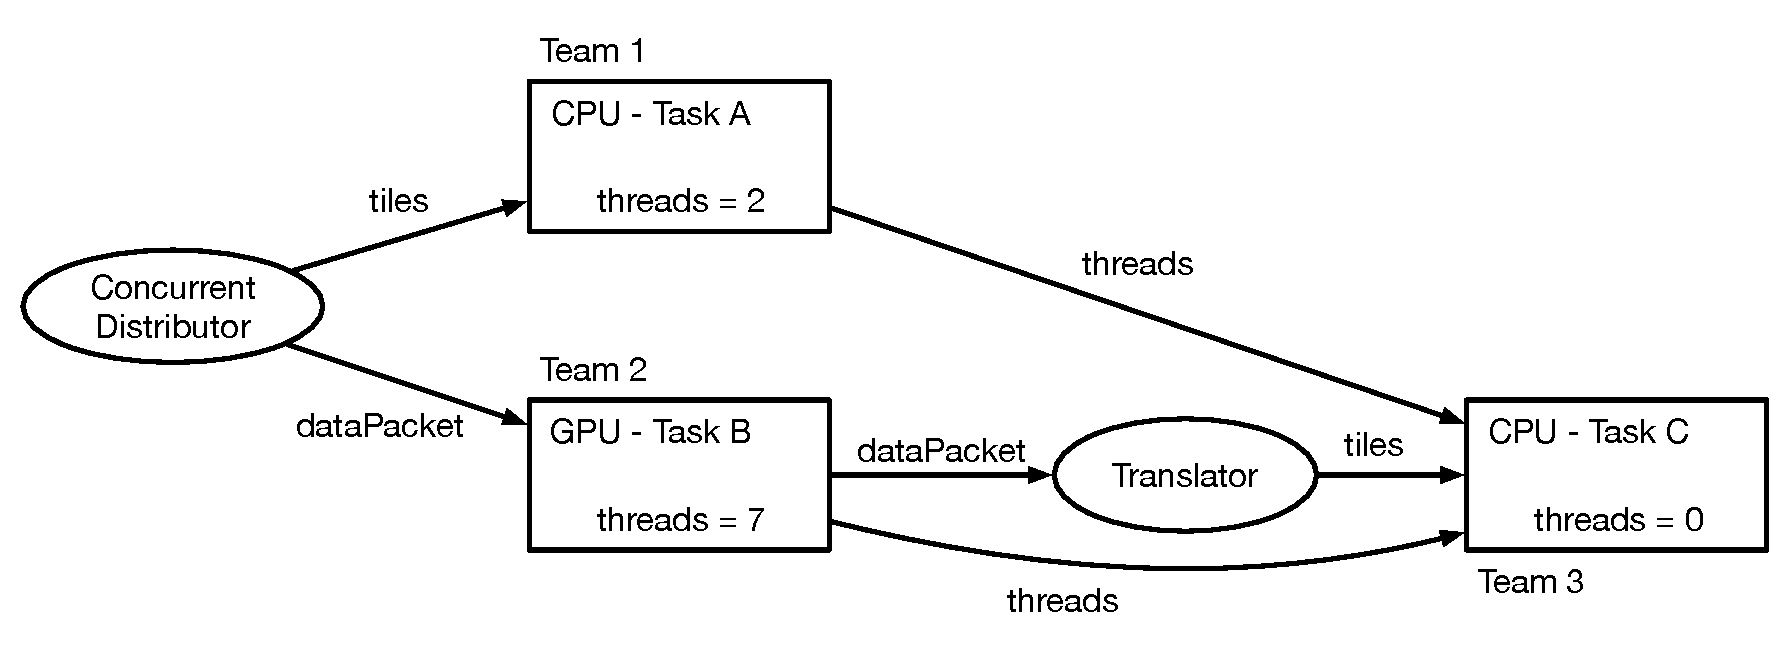
\includegraphics[width=5.5in]{ConcurrentItorExample.pdf} \caption[]{A runtime thread team configuration implementing two concurrent pipelines
using three thread teams.  In this example, routines A and C were written
with all code run in the host and  action routine B was written to launch kernels on the GPU.  The action A pipeline
runs soley on the host and is given only two threads to execute associated tasks.  The
actions B/C pipeline gives 7 threads to Team~2 to flood the
GPU quickly with data and kernels.  Once a thread in Team~2 has
applied action B to all blocks in its current data packet, the thread
enqueues the data packet on Team~2's work subscriber.  The work subscriber performs the
roles of a data mover (DM), an unpacker, and a data item splitter.  It moves the data packet asynchronoulsy back to the host, moves the data from
the host-side data packet to the appropriate location in the Grid unit's data
structures, and splits each block in the data packet into tiles and enqueues
each of these with the entity's work subscriber.  Team~3 can then apply
action C on a per-tile basis, which is optimal for execution on the host.  Since Team~3
needs pass through data from Team~2, it does not initially recieve threads.  When a thread in Team~1
or Team~2 deactivates as work winds down, the thread informs Team~3 to activate
a thread.  It follows that Team~3 could eventually have 9 activated threads for
applying action C to tiles.}
\label{fig:ConcurrentItor}
\end{center}
\end{figure}

The second layer of parallelism is forming
\textbf{\actionroutinebundles}.  Specifically, with each invocation of the \OR, the runtime interface
is designed that the code
can request application of, during the single execution cycle, one or more
actions to all data items retrieved using the iterator
specified.  In addition, the calling code informs
the \OR how to map the action routine bundle onto the node level resources.  Skillful
bundling of routines and mapping of routines to hardware enables the
runtime to efficiently use the node hardware.\\

The construction of an action routine bundle and a mapping of the bundle onto the
hardware begins by selecting actions to bundle
together.  For instance, we can identify actions A and B be
run together because the two actions do not have any data
dependencies.  For example, if A only reads and updates density and
B only reads and updates energy, then their action routines could be bundled together
and mapped on to the hardware for concurrent application.  If the mapping is onto a node with a host,
and a device with dedicated remote memory, then one action could be mapped onto
the host and the other onto the device.  In
addition, if we have a third action C that has no dependence whatsoever with either
of the first two actions or that must be run after the device action, then this
action routine may also be included in the bundle in such a way that C is only
applied to a data item after B has been applied to the item.
The two \actionroutines in a \actionroutinebundle that run concurrently
are called the \textbf{concurrent CPU \actionroutine}. A \textbf{concurrent GPU \actionroutine}
runs on nodes with host CPUs that offload to GPUs.  On a system with offloaded GPU nodes, an
\actionroutine in the bundle that is run on blocks in the CPU memory, after the concurrent
GPU \actionroutine has been applied to these blocks, is called a \textbf{post-GPU
\actionroutine}.  One can run the \OR with only one \actionroutine in the bundle
if so desired.\\

Under the hood, the \OR accepts the action routine bundle and uses the data item
iterator to gather data items on which the action routines will operate.  Each
combination of action routine and data item run is a \textbf{task}, and the execution of tasks
is orchestrated by host threads.  Therefore, this design implements task-based
parallelism using thread-level parallelism.  For the case of a node with a
host and a GPU, the thread-level parallelism refers to the orchestration of thread
execution of tasks, and execution of single tasks
on GPUs using many device threads.  Action-level parallel execution by pipelining
work on devices allows the tasks to be executed in an efficient way
across the node hardware resources.  For instance, if a \OR execution is
scheduled with the GC fill asynchronous iterator, then the stages in the
pipeline could be
\begin{enumerate}
\item{copy from the Grid unit's data structures in host memory to a host pinned memory
buffer those tiles with GC data already filled,}
\item{assemble $N$ tiles into a data packet and initiate asynchronous data
transfer to device,}
\item{launch in device all kernels that comprise the concurrent device \actionroutine and
apply to all tiles in the data packet,}
\item{transfer asynchronously all tiles in data packet back to host memory
buffer,}
\item{copy all tile data in data packet back to Grid unit's data structures in
host memory, and}
\item{apply post-concurrency host \actionroutine to all tiles in data packet.}
\end{enumerate}
If the data movements are slow, then this pipelining scheme
will allow for the overlaying of data movement with computation once the first
data packet is sent.  In the world of CPU-GPU nodes, this scheme should
enable the data movement latency hiding that is required for running efficiently
with GPUs.\\

In the concurrent CPU/GPU and post-GPU scenario, we the \OR
effectively runs two pipelines concurrently and the post-GPU \actionroutine is
an extension of the concurrent GPU \actionroutine pipeline.  The \OR uses a single
iterator over blocks to feed the two pipelines
and each block is fed to both pipelines.  Since the two pipeline implement
different chains of actions, the code that iterates and feeds
blocks identically to the pipelines is an \textbf{action parallel distributor}.\\

\begin{figure}[!ht]
\begin{center}
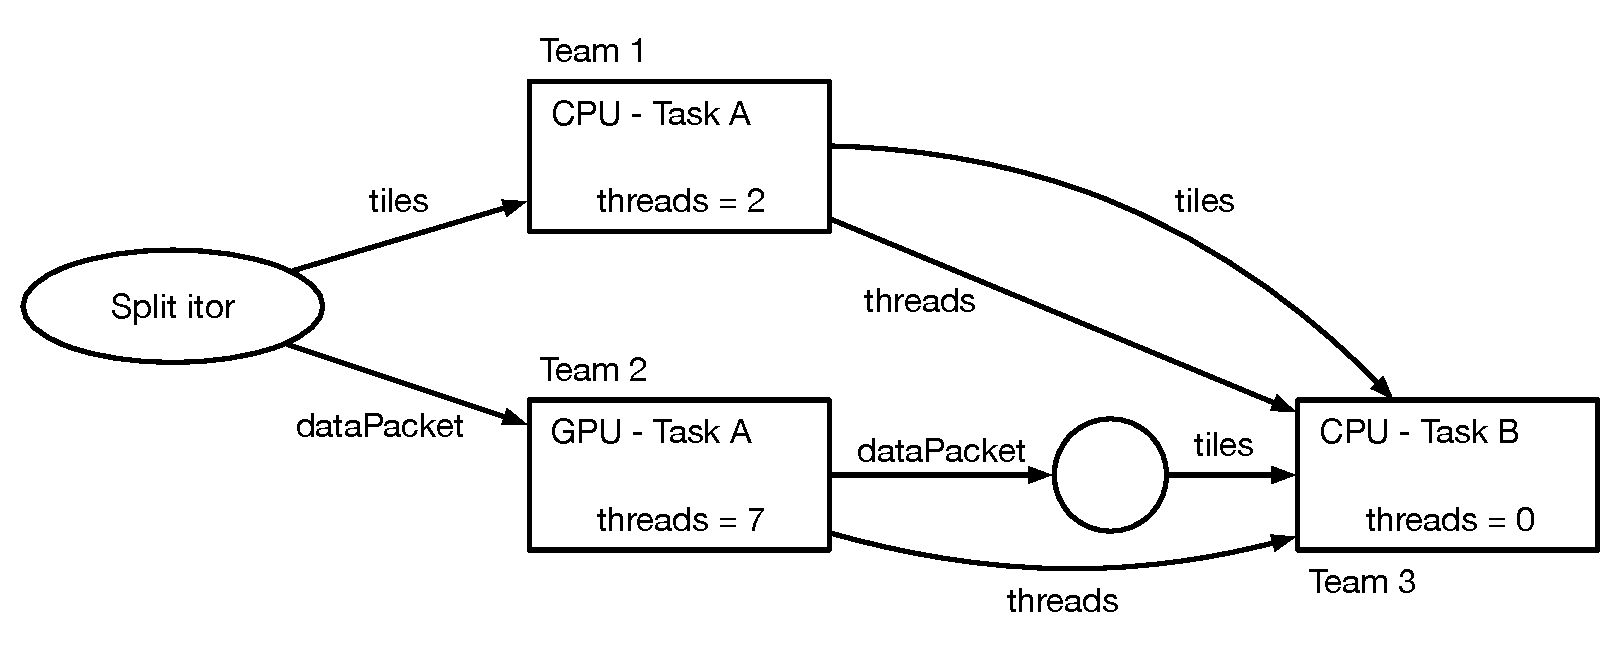
\includegraphics[width=6.0in]{WorkSplittingExample.pdf}
\caption[]{An example of a runtime thread team configuration implementing a
single, data-parallel pipeline.  The action routine bundle
mapped onto this configuration consists of an action routine that applies A
using only the host (Team 1), an action routine that applies A by launching kernels in
the GPU (Team 2), and an action routine that applies B using only the host (Team 3).  The data
parallel distributor decomposes a fraction of the blocks managed by the
runtime's MPI rank into tiles and enqueues each tile with Team~1.  The remaining
blocks are aggregated into data packets.  When a data packet is sufficiently
large, the distributor copies it asynchronously to GPU memory and enqueues it
with Team~2 so that both host and GPU are used to apply A in parallel to all
blocks managed by the runtime's MPI rank.  Both of these teams are work
publishers to Team~3 so that this team can apply action B to all tiles.  Note
that this configuration could be used if actions A and B have no data
dependencies or if action B must be applied to a tile only after action A has
been applied to the tile.}
\label{fig:SplitItor}
\end{center}
\end{figure}

\begin{figure}[!hp]
\begin{center}
\includegraphics[width=5.5in]{TaskBasedFlow.pdf}
\caption[]{A cartoon timing diagram demonstrating the evolution of a runtime
execution cycle. The cycle is given an action routine bundle composed of an action
routine that applies Action A to blocks using the host (Team 1), an action routine that
applies Action A to blocks using the GPU (Team 2), and an action routine that applies
Action B to blocks using the host (Team 3).  (This timing diagram, similar to
Figure~\ref{fig:SplitItor}, has the simplification that
Teams 1 and 3 have blocks as their data type.) The column labels $T_i$ refer to
the different threads that were activated in the different thread teams.  Each shaded
rectangular region in the diagram corresponds to one task where the color
indicates the action assigned to the task. The number inside the block is the
index of the block assigned to the task.  For the tasks executed by Team 2, the
different shades of gray indicate which blocks were grouped together into a
single data packet of four blocks.  As drawn, it appears that the block
iterator gave blocks to the data parallel distributor in order.  Even though the
first blocks were used to form the first data packet, application of Action A
started first on the host as the GPU code was penalized by the host-to-GPU data
movements.  The data movement penalties also appear occasionally as gaps between
task executions on a single thread due to the fact that the thread had to wait
for the next data packet to arrive.  The horizontal dashed lines in the Team 3
section indicates the approximate time at which blocks that have already had
Action A applied to them on the CPU or the GPU are enqueued with Team 3.  Note
that Team 3 does not immediately start applying Action B to these blocks as
Team 3 does not have any active threads until Team 2 works its way through its
tasks.}
\label{fig:TaskBasedFlow}
\end{center}
\end{figure}

The design of the \OR allows for data parallel execution of a \taskcodebundle.
For example, a CPU version and a GPU version of a single \OLAR could be
written by the offline toolchain and bundled together.  The single block
iterator in the \OR partitions the blocks, sending a fraction of blocks
to the pipeline that runs the \actionroutine on the CPU;
and the remaining blocks are sent to a second pipeline that runs the \actionroutine on the
GPU\footnote{The options are either a pre-determined, static partitioning
scheme or an online scheme that decides where to route a tile based on current
and historic load and performance telemetry data.}.  In this case, the code that
iterates over blocks and feeds the pipelines is a \textbf{data parallel
distributor}.  Another possibility is a case where the runtime uses
multiple action parallel pipelines.  However, if any one of the action parallel
``pipelines'' is actually composed of two or more subpipelines each applying the
same action, then the \OR would employ a \textbf{hybrid distributor},
capable of distributing blocks in both an action and data parallel fashion as
required.\\

The concept of \textbf{task} is an element of a high-level software model.  The design of
the \OR includes a lower-level software model element, known as a
\textbf{thread team}, used to construct runtime
pipelines mapping tasks to node hardware and allowing for load
balancing of computing resources on the host. Note that the thread teams run on the host.
At startup, the \OR will create $N$ thread teams, each of which contains $M$
threads, where $N, M$ are setup-time parameters to be determined by the offline
toolchain.\\

Each thread team contains a single queue for holding data items (to which its
action should be applied), where each data item must be of a single type.  For
example, a thread team could be constructed to only accept data items of type
tile, or to accept data items whose
type is \textbf{data packets}, comprised
of one or more tiles.While thread teams are not associated with the
different devices in a node, it is intended that a thread team whose data type
is a tile will apply its \actionroutine to all given tiles
using the CPU.  Similarly, a thread team whose data type is a data packet
 apply its task code to all given tiles using an
accelerator with its own dedicated memory. The \textbf{data packet}
exists to manage the difficulties and time penalties associated with
transferring data between host and device memories.\\

For a single \OR execution cycle, each thread team used
will be given exactly one \actionroutine in the associated \actionroutinebundle.  In addition, the thread team
is instructed to activate a given number of its $M$ threads for applying its
\actionroutine.  The activated threads apply the single \actionroutine to all units of
work, given to the team during the execution cycle, using dynamic scheduling.\\

In the action parallel example, the concurrent CPU and post-GPU
\actionroutines will be assigned to thread teams that work with tiles. The
concurrent GPU \actionroutine gets assigned to a thread team that works with data packets of
blocks\footnote{Each kernel to be executed on a GPU will be launched so that it
is applied to only a single element in a data packet.  We assume
it will be more runtime efficient for such kernel executions to
work on a block,rather than a proper subset of a block.}.  The action parallel
distributor will enqueue all tiles directly with the CPU \actionroutine's team,
aggregate blocks into data packets, and enqueue a data packet with the
concurrent GPU \actionroutine's team when each data packet contains enough
blocks or there are no more blocks left.  Upon completion of \actionroutine to
all blocks in a data packet, the concurrent GPU's team gives
ownership of the packet to a \textbf{thread team helper}.
The \textbf{thread team helper} asynchronously
transfers the data packet from the GPU memory to the host memory, moves the data
from the host-side data packet to the appropriate location in the Grid unit's
data structures, and enqueues separately each tile, of the blocks in the data
packet, with the team executing the post-GPU \actionroutine.\\

In order to hide latencies effectively and to make efficient use of node
hardware, users will choose the size of data packets
appropriately so that the \OR achieves sufficient overlap of computation and
data movement and that the devices maintain
sufficiently high occupancy.  This could include having the first data
packet contain many tiles keeping the device busy until the next round
of potentially smaller data packets arrive
in device memory.  Another important configuration detail is the total
number of data packets that will be pushed through a pipeline in an execution
cycle.  If the data packets are too large or the MPI rank has too few blocks,
then the number of data packets might be too small too overcome the
wind-up/wind-down losses of the pipeline.  A potential solution for the MPI rank
case would be to use data packets of tiles rather than data packets of blocks.\\

A design element of the \OR that can enqueue data items with a thread
team or a thread team helper is a \textbf{work publisher}.  The design elements
receiving data items in their queue are known as \textbf{work
subscribers}.  Similarly, thread teams can be configured as a \textbf{thread
publisher} and as a \textbf{thread subscriber}.  When a thread in a thread
publisher team determines that there is no more work to be done by the team in the current
execution cycle, and therefore deactivates; the thread informs the team's
subscriber that it can now activate another thread that helps the team
execute pending tasks.  This allows for some control of the load balancing of the
threads running in the host.\\

Ideally, this load balancing will extend outside of \FlashOfTheFuture to manage host
resources and third-party libraries used by the simulation.
For instance, the asynchronous iterator likely needs many threads to do its
work.  This means the total number of initial threads activated across all
thread team fed by a work distributor using this iterator, should be
low, giving the GC fill priority.  Once AMReX finishes the fill, the
work distributor can activate more threads in the teams.\\

The runtime design allows multiple types of thread team helpers, each a work
 subscriber, and some of which can also be work
publishers. \textbf{Data movers} are helpers that move a data item from one memory system to
another memory system and enqueue the data item with the mover's work subscriber.
 \textbf{Unpackers} are helpers that move the host-side
contents of a data packet to appropriate locations in the Grid unit's data
structures.  \textbf{Data item splitters} are helpers that split a data packet
into its constituent data items, and enqueues these items with the splitter's work
subscriber.  Given a data packet of blocks, a data item splitter could enqueue
on a per-tile basis, each tile of each block in
the data packet.  The \textbf{data item aggregator} helps by
accumulating individual data items and aggregating into a data packet.  When
the data packets are sufficiently large, the aggregator enqueues these with its
work subscriber.  A data item accumalator may be a work
subscriber of a thread team, whose data type is tiles.  It would accumulate
tiles, reform these in to blocks, and aggregate the blocks into data packets of
blocks.  The \textbf{data item aggregator} and \textbf{Data item splitters} function as
translators by allowing a thread team with one data type to be a work
publisher to a thread team with a different, but related, data type.  Notice that
\textbf{data mover} is a composite helper that
functions as a data mover, an unpacker, and as a data item splitter.\\

The pipeline and thread team layout pertaining to the action parallel
runtime is shown in the Figure~\ref{fig:ConcurrentItor} example.  The example of a
data parallel \OR thread team configuration is shown in
Figure~\ref{fig:SplitItor}.  The thread teams have been designed that a myriad
of \textbf{thread team configurations} can be built into the
\OR with a (potentially) different thread team configuration used for each
\OR invocation.  The specification of a thread team configuration includes the
specification of work/thread publishers and subscribers as well as the inclusion
of necessary thread team helpers (usually drawn as ovals).  We hope that this
aspect of the design allows for easily scaling the \OR's capabilities, as
node architecture grows in device diversity and in hardware complexity.  When the
offline toolchain determines how to bundle task code, we intend that the
large number of such configurations will allow for effective bundling, leading
to efficient, parallel usage of all computational in-node resources.\\

The main takeaway is that the runtime will offer \footnote{Refer to
Appendix~\ref{adx:ConfigMenagerie} for the presentation of several thread team
configurations that presently serve as use cases for designing the \OR, and
that could be offered by the \OR interface.} different thread team
configurations, each of which exposes the parallelism that is offered by node
hardware.  The code that uses the runtime must bundle action routines
wisely, and map these onto a compatible thread team configuration to allow the
action routines and bundle to capitalize on the exposed parallelism.\\

Two or more action routines are said to be \textbf{runtime-compatible} and can be
bundled together for executing in a single execution cycle if
\begin{itemize}
\item{they can be co-scheduled in the \OR such in a way that satisfies interdependencies and}
\item{the action routines are to be applied to the same set of tiles using the
same iterator}
\item{ or if all action routines are specified to apply their action to the same set of tiles but
with distinct iterators that are compatible.}
\end{itemize}
An example of the third case is when one action routine
is specified to apply its action by looping over all levels and iterating across
all leaf blocks at each level, while the other action routine is specified to
apply its action on all leaf blocks at all levels.  If the interdependencies can be
satisfied, then these two actions are runtime-compatible and when the \OR
executes the action bundle it would use a data distributor that uses the
finer-grained iterator that loops over all levels and all leaf blocks at each
level.\\

The first bulletpoint above is related to whether or not the \OR offers a thread team
configuration where the different action bundles can be mapped onto the
 teams without violating any interdependencies.
If the different routines are to be applied to different sets of
tiles,  then the routines would have to be scheduled in separate
action bundles.  The case of the concurrent-GPU and post-GPU action routines
shows that it is not necessarily the case that
runtime-compatible \taskroutines can be run concurrently.
Runtime-compatibility includes bundles of auxiliary \taskroutines
(all \taskroutines in the bundle iterate over the
empty set) and the \OR interface includes a routine for executing such a
bundle.\\

The original motivation for structuring \texttt{Driver\_evolveFlash} as a
sequence of runtime invocations of \actionroutinebundles was the desire to minimize the
number of data movements between host and devices.  As part of arriving at this
goal, we determined that \textbf{data movements} (\textit{e.g.} intranode,
internode, or host-to-accelerator) be first class members of an
operation's algorithm and be expressed at the highest-level
representation of the operation (\eg, \texttt{Hydro.F90}), instead of
residing in a function call deep in the operation's call stack.  We design for the physics
 units to be restructured by unit developers to exploit data movements and to
 uncover the largest blocks of code that can be run between data
movements (\textit{i.e.} the action regions).

\\

The current implementation of the \texttt{simpleUnsplit} Hydro code contains
 an example of an implicit barrier that can exist between
consecutive task regions.
Consider solution advance phase $n+1$, which takes the solution from state $n$ to state $n+1$.
When tiling is not enabled, the solution at state $n$, on
a given block, can be used to compute fluxes; and these can then be used to overwrite in-place
the solution data, with that of the $n+1$ state on the same block.  In other
words, the compute flux and update solution \OLAR, originally present in
two separate \actionnests, can be fused into one
computation to be done in one iteration in a single \actionnest.\\

When proper tiling is enabled, the solution data cannot always be overwritten
in-place, as this could update the data in interior cells, that are in fact
guardcells of a different proper tile.  If this is done before the fluxes have been
computed in the neighboring tile, then the result will not be correct.
In this occurance, the compute fluxes \actionroutine must be run on all tiles, and
its output (in this case, face-centered tile data) saved in intermediate storage before
 the solutions are updated based on the fluxes.
This saving in intermediate storage is an implied and required barrier that exists between
the two \actionnests, and that prevents combining the two \OLARs into a single
\OLAR in a single \actionnest.\\

% Consider the case of a loop over tiles that sets a value to a variable and
% where the value can only be determined after iterating over all tiles (i.e.
% something akin to a reduction).  If a second loop over the same tiles uses
% that variable, then an implied variable exists.

We say two or more \taskroutines can be
\textbf{fused} if
\begin{enumerate}
\item{the \taskroutines are to be run on the same set of tiles or if one \taskroutine
iterates over tiles at a finer-grained structure and the second \taskroutine can
complete its work on its set of tiles using the same structure and}
\item{they have no data dependencies or appear in order in the \AKG with
no implicit barrier between them.}
\end{enumerate}
This definition allows for fusing \taskroutines from different operations and even from
different units.
It might be more advantageous in terms of decreased runtime
to avoid fusing to enable the \taskroutines to run on different hardware.  Also,
fusion could lead to performance degradation if the register pressure is too
high for the fused \taskroutine and frequent context switching is required by the data
access pattern.\\

If the inclusion/exclusion of a data movement or barrier in a simulation depends
on parameters known at configuration time, then parameter values that result in
exclusion should be used by the toolchain to fuse \taskroutines originally separated by
the barrier or data movement.  This implies that the highest-level expression of
an operation should include all such barriers and data movements along with the configuration-time parameters (refer to
Figure~\ref{fig:simpleUnsplitKernelGraph}).  As a result of this design, developers of
units with complex execution paths only need to write a single high-level
description of the unit.\\

Runtime-compatible \taskroutines having no interdependence within a single
solution advance phase can be bundled together.

Also, we can choose to fuse independent \taskroutines in any
desired order.  Runtime-compatible \taskroutines that have a dependence can be bundled
together in the same \OR execution, as long as the mapping of \taskroutines onto
teams in a specific thread team configuration maintain the correct order of
operation.\\

Finally, we partition the code used in each solution advance phase into the three classes
\begin{enumerate}
\item{\texttt{Driver\_evolveFlash} and its auto-generated \OR calls,}
\item{\textbf{static Fortran routines} that carry out computations at the
level of a tile (\textit{e.g.} \texttt{hy\_computeFluxes}), and}
\item{the \textbf{patch panel} layer of code that must be auto-generated to
match the contents of \texttt{Driver\_evolveFlash} to the interfaces of the
static Fortran routines.}
\end{enumerate}
If a simulation is to be run in CPU-only mode, then the patch panel class of files
would consist of auto-generated high-level representations of each operation
(\textit{e.g.} \texttt{Hydro.F90}), that are functionally equivalent to the code presently
in \FlashOfTheFuture.  Otherwise these files would be auto-generated Fortran files that
implement each of the \taskroutines being passed to an \OR execution.\\


%%%%%----- ORCHESTRATION SYSTEM HIGH-LEVEL REQUIREMENTS -----%%%%%
\section{Overall System}
\subsection{Requirements}

\begin{req}
The orchestration system implementation and dependencies shall not impede \FlashOfTheFuture
from being used on *nix operation systems including macOS nor from being run for
research on laptops.  Implementations shall not require more than the C++11
standard. Threading implementations shall be portable across platforms that
conform to the aforemented operating systems.
\end{req}

\begin{req}
If a simulation is set up such that no Orchestration runtime is needed, then the
\OR shall not be built into the simulation.  In particular, this means that
there shall be no unnecessary resources allocated, no extra level of packing
tiles into data packets, and no unnecessary configuration complexity.  This
could allow for basic stub implementations such as initialization/finalization
being called from Driver.
\end{req}

It is possible that users might want to run a simulation on a CPU-only platform
using the \OR so that independent \taskroutines or independent task regions/communications
can be overlaid.

\begin{req}
At any point in time during the execution of a simulation, there shall be no more
than one instance of the \OR in operation so that design complexity can
be minimized (\textit{e.g.} resource allocation and management).
\end{req}

\begin{req}
\label{req:UnitImplementations}
The \OR shall be built into \FlashOfTheFuture as a new unit and the unit shall allow
for different implementations of the unit.  Some examples of different
implementations will be
\begin{itemize}
\item{low-level (\textit{e.g.} CUDA) \textit{vs.} high-level
(\textit{e.g.} OpenMP) and}
\item{general (\textit{e.g.} CUDA) \textit{vs.}} platform-specific
(\textit{e.g.} CUDA optimized for Summit).
\end{itemize}
\end{req}

\begin{req}
\label{req:Portability}
All implementations shall be designed for portability.  For example,
\textit{general} use GPU-related code shall avoid using device-specific library
functionality (managed memory). Other GPU-based platforms might not
offer portable managed memory or may not have managed memory.
\end{req}


\begin{req}
The interface of the \OR shall be designed such  that when a new type of
device is introduced in platform nodes, the routines for starting an \OR
execution cycle can be extended trivially\footnote{Ideally by adding new function
pointers to the parameter list of these routines.} for including the running of
\taskroutines on these devices.  If the nodes allow concurrently running of \taskroutines on
the device while running code on the host (or on other devices), then the updated
interface shall allow for this.
\end{req}

\begin{req}
The system shall be comprised of
\begin{enumerate}
\item{an offline tool that constructs an \AKG,}
\item{an offline tool that optimizes resource use and execution time by
determining both how to order \taskroutines and on which hardware to run each
\taskroutine; thus creating the ability to form \taskcodebundles,}
\item{offline tools that generate simulation- and platform-specific Fortran code
based on the optimized scheduling of the previous tool, and}
\item{an orchestration runtime subsystem (\shortOR).}
\end{enumerate}
\end{req}
For more information regarding each of these subsystems,
refer to detailed design section below.\\

The \spelledoutAKG shall represent only the work that needs to be done
during each occurrence of a solution advance phase. %%each time step.
The information needed to construct the \AKG shall
be made available at setup time so that the graph can be constructed offline at
setup time, which implies that the graph is static and valid for each
each occurrence of a solution advance phase.\\

The design shall allow for specification of runtime parameters that can alter
how the \AKG is traversed at runtime.\\

The design shall allow for executing code between solution advance phases, including
computationally-heavy code, that can make use of the \OR.
However, this code shall not require automatic optimization of scheduling nor
auto-generation of code, and shall therefore not be included in the \AKG.
  An example is the regridding of the domain by an AMR-based
implementation of the Grid unit.\\

\begin{req}
\label{req:NonORCodeInDriverEvolveFlash}
Users and code contributors may desire to build a simulation with
computation-heavy code that does not conform to the needs
of the \OR interface (\textit{e.g.} libraries such as
Thornado that need to be useable by many applications).  The orchestration
system shall allow such code to be run directly by calls in
\texttt{Driver\_evolveFlash} between \OR execution cycles.
\FlashOfTheFuture shall allow such code to be run
\begin{itemize}
\item{as serial code,}
\item{as code that manages and coordinates parallel execution internally, or}
\item{that is parallelized through another performance portability layer such as
Kokkos or Raja.}
\end{itemize}
\end{req}

While it could be possible to run concurrently the final \taskroutines from the
solution advance phase $n^{th}$
with the beginning \taskroutines for solution advance phase $n+1$, the orchestration
system shall not allow for such parallelism so that complexity is reduced.\\

The system shall be designed such that the bundling of action regions and relative
scheduling of these can be done either as a static task at setup time (bundling of \OLARs), or at
runtime (bundling of \actionroutines) to enable bundling and scheduling be done dynamically in response to
acquiring actual runtime performance and resource usage data during a simulation
run.  Principally, this means that the breaking down of the offline toolchain into
individual tools must be done to allow for this.
Therefore, care needs to also be taken when establishing the interfaces between
these tools.  \\

When the optimization of task/kernel scheduling is done at runtime, the
code generation tool shall write at setup time Fortran code that will allow a
forecasting scheduler to execute each solution advance phase with as many \actionroutinebundles as it
sees fit.\\

Ideally, the public interface of the \OR shall not need to be
altered to accommodate running with static scheduling or runtime scheduling.\\

At each regridding, the Grid unit shall use the \OR to cache
non-tile-specific information in device memory.  Examples of such information
are
\begin{itemize}
\item{cell and face coordinates,}
\item{face areas, }
\item{cell volumes, and}
\item{[XYZ] mesh sizes.}
\end{itemize}
This information shall not change during the computations made in a single solution
advance phase so that available memory resources in different devices are fixed when the
solution advance phase starts.\\

Values that are needed in device memory for computation and that are constant
during a single solution advance phase shall stored in host memory, and in all device memory
(where needed) at the beginning of the solution advance phase such that the value is
correctly mirrored across all memory systems, and such that memory usage can be
correctly gauged by the runtime system at the start of each solution advance phase.

%%%%%----- STATIC FORTRAN CODEBASE -----%%%%%
\section{Static Fortran computational code}
\subsection{Requirements}
The routines defined in the static Fortran computational code shall each operate
on a single tile or on no tile at all.\\

The routines defined in the static Fortran computational code shall not
dynamically allocate memory.  Rather, the necessary tiles of memory shall be
passed in from the highest-level of such routines.  In other words, all memory
management is done at the level of each operation and the tiles of scratch
memory needed by each static routine and all its subroutines must be passed into
the static routine and passed through the interface to the subroutines.

\subsection{Desired Requirements}
The static Fortran routines shall not be exposed to the notion of a tile and
therefore shall not contain the Grid unit's tile descriptor as a parameter.
Rather, all tile-specific information shall be obtained from the Grid unit by
the operation at the highest level and all such information passed to static
Fortran routines as individual parameters.  This shall be implemented so that
Grid information cached in device memory can be used immediately within device
kernels.

%%%%%----- ORCHESTRATION OFFLINE TOOLCHAIN -----%%%%%
\section{Offline Toolchain}

\subsection{Introduction}

The offline toolchain is comprised
of an annotated kernel graph constructor, a task scheduler, and a code
generator and assembler.  These tools %are connected in such a way that they
form a pipeline that converts a collection of high-level expressions of
operations from the solution advance phase, into the Fortran
%expression  of the solution advance phase in the form of
code of
\code{Driver\_evolveFlash} and the patch code
%needed to get this file patched into the static Fortran code layer \textit{via}
connecting static Fortran with
the runtime.\\

%In a realistic use scenario, the expression of
The work to be done during the solution advance
phase is a collection of high-level mathematical activities
that comprise \FlashOfTheFuture users simulation components.
The offline toolchain translates these high-level operations, at each stage in
the toolchain,
%and translates each expression of the computational work
into expressions that are increasingly concrete (lower-level) and adapted to the
hardware.  Our design is human readable output between
tools in the toolchain
%, the product that links tools (\ie, the output
%of one tool is the input to the next) should be
is
and human creatable allowing users
to debug the toolchain by injecting their own test case.\\

The first tool in the toolchain, the annotated kernel graph
constructor, will require that physics unit developers encode their operations in a
simplified, concise language that expresses the underlying algorithm, taking input in terms of
data movements/barriers. The code that must be executed between the actions
also needs to be clear and concise.  We explore the possibility that this simple language be
implemented with a dictionary where the value is associated to each key in the
dictionary.  We plan for the keys to point to associated static Fortran routines.
 The dictionary is a mapping of the developer's concept of the action to the
actual Fortran routine applying the action to data (\ie, the associated
\textbf{action routine}).  This scheme does require
that these developers will need to add their own $(key, value)$ pairs to the
dictionary.\\

The \textbf{annotated kernel graph constructor}, using standard compilation
techniques and tools, generates for
each operation to be run during the solution advance phase, an annotated kernel
graph.  If the dictionary maps concept to actual Fortran implementation, then
this tool could use the Fortran listing to identify kernels,
 and extract the data needed for
the annotations.  The tool will look at given setup-time
parameters and determine how this information can be used to simplify the kernel
graphs and potentially expose where individual actions could be fused into
larger actions.\footnote{\Jared{I think that it would be premature for this tool
to actual do the fusing.  Rather, I think that the task scheduler should do this
as it might determine that by \emph{not} fusing two actions, it might find a
particular set of action bundles that could be more performant.  Therefore, this
tool's job is just to simplify.}
\JaredRfromKW{I agree that tool~\#1 should not do any fusing or similar transformations.
It should, however, be able to evaluate some logical conditions used for conditional
configuration (\emph{if} all the inputs to the conditions are known at the time the tool runs)
and eliminate some code (together with the relevant conditional controls) accordingly.
For example, tool~\#1 could remove some conditional barriers.}}  The annotated kernel graphs could be output
in a standard format such as the DOT graph description language.

Or the annotated kernel graphs could be output
as a stream of lines of Fortran code with interspersed lines of special marks
that denote special points and/or attached information.
\\

The annotated kernel graphs should include annotations about data
usage, that can be used by later tools in the chain to identify data
dependences.  Ideally, we will have a distinct helper tool in the offline
toolchain that can scan action routines, determine the data usage information,
and place these in special data usage files in the \FlashOfTheFuture folder
hierarachy.  These could (potentially) be written by the helper every time code
is altered in the repository.  These data usage files are then maintained
up-to-date and would be consistent with the data usage
expressed in Fortran in the actual implementation.  There would then be little
maintenance of these files and a low possibility of error due to inconsistency.
By encoding these as files in the folder hierarchy and in a human readable
format, we provide developers with the ability to check that the dependences
are correct and allow for general debugging.  These files could be included in the
dictionary mapping of action to action routine as an extra source of data
for annotations.\\

The task scheduler would be given the collection of all annotated kernel graphs
and use standard task scheduling runtimes in an offline tool such as StarPU
or Apple's GCD to determine how to bundle actions together for running with the
orchestration runtime.  This would include determining simultaneously which
thread team configuration should be used for each bundle.  As part of this
process, the annotated kernel graphs will need to be converted into a similar
data structure as dictated by the input requirements of GCD or StarPU.  The
output of this task scheduler could be a textual version of a rich data
structure expression of \code{Driver\_evolveFlash}.  For example, it could be a
single JSON-format file that contains (in order) each action bundle and the code
to be run between bundles.  In addition, each action bundle in this file would
be a rich data type that characterizes the bundle (\eg, the iterator to use, the
actions to run, the mapping of actions to thread teams in a specified thread
team configuration).\\

The general guiding principle for the optimization done by the scheduler is to
make the most efficient and complete use of node resources with the caveat that
we can sometimes sacrifice node resource usage if runtime execution times improve
significantly.  For instance, the thread team design presently has a lower bound
on kernel execution times.  If a kernel has a run time
below this limit, then there might be some speed-up, but the runtime won't be
making efficient use of the hardware.  Therefore, the task scheduler might
decide to fuse two quick action routines into an action routine whose run time is larger
than the lower bound.  Or it might choose to schedule the quick routines alone
with the understanding that they aren't efficient, but at least we are using all
the hardware.  The task scheduler might also be required to fuse
kernels within a single action where possible.  It could occur that fusing two
quick actions would lead to a larger action that could be run efficienctly by
the \OR.  There might be cases where fusing kernels could lead to an
optimized run time that is shorter than the lower bound.  In these cases, the
kernel fuse optimization would lead to inefficiency.\\

Suppose that a single operation needs to cache large tables in device
memory throughout the duration of the simulation.  These could be static or
updated.  If these tables are large enough that they limit the number of blocks that can be
stored simultaneously in the device memory, then runtime performance would
suffer.  Then the task scheduler could look at the memory requirements
per block (\ie, the size of the block itself and all extra and scratch data
needed for that block), the size of the tables, and the size of the device
memory to determine how to schedule the actions that use the table.  For
instance, it could choose to always run this action in the host so that the
tables are never in device memory.  Also, it could program a prefetch of the
tables from host to device memory just before the action bundle with the routine
is run.  Similarly, the previous action bundle could be created so that it
contains an action that regenerates the table in device memory.\\

The code generator would ingest the JSON-format file, write the actual
\code{Driver\_evolveFlash} in Fortran as well as the code that patches the
orchestation runtime to the static Fortran code so that these are passed the
correct arguments.\\

%The composer should have four levels of hierarchy, with each hierarchy
%having its own set of meta information encodings. The meta information
%encoded should be such that the composer tool can infer dependencies
%easily.

\subsection{Code Generation and Assembly}
\label{sec:code-generation}

This is the final step in the offline toolchain that will generate
static Fortran code through code transformation where needed, and
assemble the whole application by combining it with existing static
Fortran code. The expectation is that the arithmetic and low level
logic will continue to be maintained in Fortran augmented with
keys. The keys could be macros or directives. Some keys may be there
strictly for reducing lines of code by expressing repeated patterns as
micros, while other keys may be useful in optimization for target
platforms. For example invoking the iterator and assembling the
meta-information of a block or a tile is a code pattern that is
repeated in all physics units. It is a simple matter to replace this
pattern with a known key. This way it is less error prone, and it is
far easier to modify the iterators themselves as needed without
intrusive modifications in the source files. An example of using a key
for optimization might be some code that comes into play only when
certain conditions are met. With a properly designed keys combined with
hints that can be encoded in {\it recipes}, branches may be eliminated
deep in loop-nests.

The term {\it recipes} refers to
hints that can either be encoded by the \PUD or extracted by a tool
that indicate what semantic constraints have been exercised and what
liberties can be taken by the code transformation tools for
optimization. Conceptually, recipes serve the same purpose for
assembling a function from sub-functional code fragments that
\code{Config} files do for assembling a unit for execution from a
collection of functions and subroutines. One way to think of how
recipes may work is to associate code snippets with keys. Different
implementations of the function can be generated by using the keys in
different order, as long as each order is consistent with expected outcome of the
function.

The first example illustrates the use of keys acting as macros that
make the code more readable, and allows a simple optimization of
eliminating a branch from a loop nest
\begin{verbatim}

do k = limitsPlus(LOW,KAXIS), limitsPlus(HIGH,KAXIS)
    do j = limitsPlus(LOW,JAXIS), limitsPlus(HIGH,JAXIS)
       do i = limitsPlus(LOW,IAXIS), limitsPlus(HIGH,IAXIS)
           ! calculate magnitude of g
           magg = gvec(IAXIS,i,j,k)**2
           if (NDIM>=2) magg = magg+gvec(JAXIS,i,j,k)**2
           if (NDIM==3) magg = magg+gvec(KAXIS,i,j,k)**2
           magg = sqrt(magg)

           ! for these options we need costheta
           if (fl_fsBuoyCompSuppress .or. fl_fsGcdFlameSuppress) then
              select case (fl_fsGeom)
              case (CARTESIAN)
                costheta = kCoord(k)/sqrt(iCoord(i)**2+jCoord(j)**2+kCoord(k)**2)
              case (CYLINDRICAL)
                 costheta = jCoord(j)/sqrt(iCoord(i)**2+jCoord(k)**2)
              case default
                 call Driver_abortFlash("bad geometry for angle-based suppression")
              end select
           endif
      end do
   end do
end do
\end{verbatim}
We next define a few keys.

\begin{verbatim}
loopnest_limitsPlus =
do k = limitsPlus(LOW,KAXIS), limitsPlus(HIGH,KAXIS)
    do j = limitsPlus(LOW,JAXIS), limitsPlus(HIGH,JAXIS)
       do i = limitsPlus(LOW,IAXIS), limitsPlus(HIGH,IAXIS)

loopnest_end =
      end do
   end do
end do

calc_mag =
  ! calculate magnitude of g
   magg = gvec(IAXIS,i,j,k)**2
   if (NDIM>=2) magg = magg+gvec(JAXIS,i,j,k)**2
   if (NDIM==3) magg = magg+gvec(KAXIS,i,j,k)**2
   magg = sqrt(magg)

\end{verbatim}

We can now rewrite the code a lot more succinctly as follows.
\begin{verbatim}

    @key loopnest_limits_plus
     ! calculate magnitude of g
        @key calc_mag
        ! for these options we need costheta
        if (fl_fsBuoyCompSuppress .or. fl_fsGcdFlameSuppress) then
           select case (fl_fsGeom)
           case (CARTESIAN)
              costheta = kCoord(k)/sqrt(iCoord(i)**2+jCoord(j)**2+kCoord(k)**2)
           case (CYLINDRICAL)
              costheta = jCoord(j)/sqrt(iCoord(i)**2+jCoord(k)**2)
           case default
              call Driver_abortFlash("bad geometry for angle-based suppression")
           end select
        endif
    @key loopnest_end
\end{verbatim}

Next we can optimize it as follows.
\begin{verbatim}

 select case (fl_fsGeom)
 case (CARTESIAN)
   @key loopnest_limits_plus
      @key calc_mag
       costheta = kCoord(k)/sqrt(iCoord(i)**2+jCoord(j)**2+kCoord(k)**2)
   @key loopnest_end
 case (CYLINDRICAL)
   @key loopnest_limits_plus
      @key calc_mag
          costheta = jCoord(j)/sqrt(iCoord(i)**2+jCoord(k)**2)
   @key loopnest_end
 case default
      call Driver_abortFlash("bad geometry for angle-based suppression")
 end select
\end{verbatim}

The decorated code here is not only cleaner, and more maintainable,
but the optimized version is also guaranteed to be without a branch inside the loop that a
compiler may or may not have recognized as optimizable. A
more complex example illustrates how recipes may be used to encode
hints. Here a few keys have already been assumed such as bounds for
1D and 3D arrays.

\begin{verbatim}
allocate(atwood(@KEY bounds_limits_plus_3d)istat=stat)
allocate(dens( @KEY bounds_limits_plus_3d)istat = stat)
allocate(gvec(NDIM, @KEY bounds_limits_plus_3d)istat = stat)
allocate(gpot( @KEY bounds_limits_plus_3d),istat=stat)
if (fl_fsUseTFI) then
    allocate(quench_limit( @KEY bounds_limits_plus_3d)istat = stat)
endif

  ! get necessary coordinates depending on options and geometry
  if (fl_fsBuoyCompSuppress .or. fl_fsGcdFlameSuppress) then
     select case (fl_fsGeom)
     case (CARTESIAN)
        allocate(iCoord(@KEY bounds_limits_plus_x)istat=stat)
        allocate(jCoord( @KEY bounds_limits_plus_y)istat=stat)
        allocate(kCoord( @KEY bounds_limits_plus_z)istat=stat)
        call Grid_getCellCoords(IAXIS,CENTER,level, limitsPlus(LOW,IAXIS), limitsPlus(HIGH,IAXIS), iCoord)
        call Grid_getCellCoords(JAXIS,CENTER,level, limitsPlus(LOW,JAXIS), limitsPlus(HIGH,JAXIS), jCoord)
        call Grid_getCellCoords(KAXIS,CENTER,level, limitsPlus(LOW,KAXIS), limitsPlus(HIGH,KAXIS), kCoord)
     case (CYLINDRICAL)
        allocate(iCoord(@KEY bounds_limits_plus_x)istat=stat)
        allocate(jCoord( @KEY bounds_limits_plus_y)istat=stat)
        call Grid_getCellCoords(IAXIS,CENTER,level, limitsPlus(LOW,IAXIS), limitsPlus(HIGH,IAXIS), iCoord)
        call Grid_getCellCoords(JAXIS,CENTER,level, limitsPlus(LOW,JAXIS), limitsPlus(HIGH,JAXIS), jCoord)
     case default
        call Driver_abortFlash("bad geometry for angle-based suppression")
     end select
  endif

  ! this returns laminar flame speed and estimate of unburned density at this pressure
  call fl_fsLaminarFlameSpeedBlock(Uin, flamespeed, dens,  &
                                   limitsPlus, flamewidth)
  ! this accounts for Turbulence-Flame Interaction
  if (fl_fsUseTFI) &
    call fl_fsTFIFlameSpeedBlock(Uin, flamespeed, flamewidth, dx, &
      limitsPlus, quench_limit)
  ! get atwood number estimate
  call fl_fsAtwood(Uin, atwood, dens, limitsPlus)
  ! calculate gravitational acceleration
  ngcellplus=ngcellplus+fl_gsOrder

  gpot(1, @KEY bounds_limits_plus_3d) = &
     Uin(GPOT_VAR,@KEY bounds_limits_plus_3d)

  call Gravity_accelOneBlock(gpot,gvec,limitsPlus,deltas,fl_fsGeom)
  deallocate(gpot)
  ! now calculate buoyancy-compensated flame speed
  ngcellplus=ngcellplus_in
  @KEY loopnest_limits_plus
      @KEY calc_mag
         ! for these options we need costheta
           if (fl_fsBuoyCompSuppress .or. fl_fsGcdFlameSuppress) then
              select case (fl_fsGeom)
              case (CARTESIAN)
                costheta = kCoord(k)/sqrt(iCoord(i)**2+jCoord(j)**2+kCoord(k)**2)
              case (CYLINDRICAL)
                 costheta = jCoord(j)/sqrt(iCoord(i)**2+jCoord(k)**2)
              case default
                 call Driver_abortFlash("bad geometry for angle-based suppression")
              end select
           endif

           ! this is the 0.5*sqrt(A g m Delta) flame speed
           if (fl_fsBuoyCompSuppress .and.  &
               time > fl_fsBuoyCompSuppressTime .and. costheta <= fl_fsBuoyCompSuppressCosTheta ) then
              bcspeed = 0.0
           else
              bcspeed = 0.5*sqrt( atwood(i,j,k)*magg*fl_fsMDelta)
           endif

           if (fl_fsUseTFI) then
              if (quench_limit(i,j,k) > 0.0) then
                 bcspeed = min( quench_limit(i,j,k), bcspeed)
              endif
           endif

           ! recall flame speed is currently set to laminar (or turbluent) speed
           flamespeed(i,j,k) = max( flamespeed(i,j,k), bcspeed)

           ! quench flame at low densities if requested
           if (fl_fsQuench) then
              if (dens(i,j,k) < fl_fsQuenchDens0) then
                 flamespeed(i,j,k) = 0.0
              else if (dens(i,j,k) < fl_fsQuenchDens1) then
                 x = ( dens(i,j,k) -fl_fsQuenchDens0)*fl_fsQuenchInvDDens
                 flamespeed(i,j,k) = (3.0*x-2.0*x**2)*x*flamespeed(i,j,k)
              endif
           endif

           !  Suppress flame in selected region
           if ( fl_fsGcdFlameSuppress .and. &
                time > fl_fsGcdFlameSuppressTime .and. costheta <= fl_fsGcdFlameSuppressCosTheta ) then
                flamespeed(i,j,k) = 0.0
           endif
  @KEY loopnest_end
\end{verbatim}

We define a few more keys.
\begin{verbatim}
allocate_3d =
allocate(atwood(@KEY bounds_limits_plus_3d)istat=stat)
allocate(dens( @KEY bounds_limits_plus_3d)istat = stat)
allocate(gvec(NDIM, @KEY bounds_limits_plus_3d)istat = stat)
allocate(gpot( @KEY bounds_limits_plus_3d),istat=stat)
if (fl_fsUseTFI) then
     allocate(quench_limit( @KEY bounds_limits_plus_3d)istat = stat)
endif

deallocate_3d =
deallocate(atwood)
deallocate(dens)
deallocate(gvec)
deallocate(gpot)
if (fl_fsUseTFI) then
     allocate(quench_limit)
endif

laminar_speed =
call fl_fsLaminarFlameSpeedBlock(Uin, flamespeed, dens,  &
                                   limitsPlus, flamewidth)


Turbulent_interation =
  ! this accounts for Turbulence-Flame Interaction
  if (fl_fsUseTFI) &
    call fl_fsTFIFlameSpeedBlock(Uin, flamespeed, flamewidth, dx, &
      limitsPlus, quench_limit)

Atwood =
  ! get atwood number estimate
  call fl_fsAtwood(Uin, atwood, dens, limitsPlus)

Gravitational_acceleration =
  ! calculate gravitational acceleration
  ngcellplus=ngcellplus+fl_gsOrder
  gpot(1, @KEY bounds_limits_plus_3d) = &
     Uin(GPOT_VAR,@KEY bounds_limits_plus_3d)
  call Gravity_accelOneBlock(gpot,gvec,limitsPlus,deltas,fl_fsGeom)
  ! now calculate buoyancy-compensated flame speed


get_coord_3d =
  allocate(iCoord(@KEY bounds_limits_plus_x)istat=stat)
  allocate(jCoord( @KEY bounds_limits_plus_y)istat=stat)
  allocate(kCoord( @KEY bounds_limits_plus_z)istat=stat)
  call Grid_getCellCoords(IAXIS,CENTER,level, limitsPlus(LOW,IAXIS), limitsPlus(HIGH,IAXIS), iCoord)
  call Grid_getCellCoords(JAXIS,CENTER,level, limitsPlus(LOW,JAXIS), limitsPlus(HIGH,JAXIS), jCoord)
  call Grid_getCellCoords(KAXIS,CENTER,level, limitsPlus(LOW,KAXIS), limitsPlus(HIGH,KAXIS), kCoord)


get_coord_2d =
   allocate(iCoord(@KEY bounds_limits_plus_x)istat=stat)
   allocate(jCoord( @KEY bounds_limits_plus_y)istat=stat)
   call Grid_getCellCoords(IAXIS,CENTER,level, limitsPlus(LOW,IAXIS), limitsPlus(HIGH,IAXIS), iCoord)
   call Grid_getCellCoords(JAXIS,CENTER,level, limitsPlus(LOW,JAXIS), limitsPlus(HIGH,JAXIS), jCoord)

do_quenching =
      ! this is the 0.5*sqrt(A g m Delta) flame speed
       if (fl_fsBuoyCompSuppress .and.  &
           time > fl_fsBuoyCompSuppressTime .and. costheta <= fl_fsBuoyCompSuppressCosTheta ) then
          bcspeed = 0.0
       else
          bcspeed = 0.5*sqrt( atwood(i,j,k)*magg*fl_fsMDelta)
       endif
        if (fl_fsUseTFI) then
          if (quench_limit(i,j,k) > 0.0) then
             bcspeed = min( quench_limit(i,j,k), bcspeed)
          endif
       endif

        ! recall flame speed is currently set to laminar (or turbluent) speed
       flamespeed(i,j,k) = max( flamespeed(i,j,k), bcspeed)

       ! quench flame at low densities if requested
       if (fl_fsQuench) then
          if (dens(i,j,k) < fl_fsQuenchDens0) then
             flamespeed(i,j,k) = 0.0
          else if (dens(i,j,k) < fl_fsQuenchDens1) then
             x = ( dens(i,j,k) -fl_fsQuenchDens0)*fl_fsQuenchInvDDens
             flamespeed(i,j,k) = (3.0*x-2.0*x**2)*x*flamespeed(i,j,k)
          endif
       endif
        !  Suppress flame in selected region
       if ( fl_fsGcdFlameSuppress .and. &
            time > fl_fsGcdFlameSuppressTime .and. costheta <= fl_fsGcdFlameSuppressCosTheta ) then
            flamespeed(i,j,k) = 0.0
       endif


\end{verbatim}


The code above can be turned into
\begin{verbatim}

## HINT non-local
  @key allocate_3d
  ! this returns laminar flame speed and estimate of unburned density
at this pressure

##HINT overlap
 @key laminar_speed
 @key turbulent_interaction
 @key Atwood
 @key gravitational acceleration
## end HINT

 @key laminar_speed
 @key turbulent_interaction
 @key Atwood
 @key gravitational acceleration


  ngcellplus=ngcellplus_in

  ! get necessary coordinates depending on options and geometry
  if (fl_fsBuoyCompSuppress .or. fl_fsGcdFlameSuppress) then
   select case (fl_fsGeom)
   case (CARTESIAN)
   @key get_coord_3d
   @key loopnest_limits_plus
      @key calc_mag
       costheta = kCoord(k)/sqrt(iCoord(i)**2+jCoord(j)**2+kCoord(k)**2)
      @key do_quenching
   @key loopnest_end
 case (CYLINDRICAL)
   @key get_coord_2d
   @key loopnest_limits_plus
      @key calc_mag
          costheta = jCoord(j)/sqrt(iCoord(i)**2+jCoord(k)**2)
      @key do_quenching
   @key loopnest_end
 case default
      call Driver_abortFlash("bad geometry for angle-based suppression")

  @KEY loopnest_end
@Key deallocate_3d
\end{verbatim}

In the code above the first hint, that the arrays are non-local
indicates to the code optimizer that these arrays are used as
arguments in calls from within this function, so their scope is not
limited to this function. The second hint about overlap indicates that
there are no write conflicts in these functions so they can be
launched on different threads in a multicore system.

\subsection{An Exercise to Demonstrate an Offline Pipeline}
\label{sec:offline-pipeline-demo}

We demonstrate what the input and output files at each stage
of the offline toolchain can look like.  Figure~\ref{fig:offline-toolchain-ex}
gives an overview.
The presented concepts are demonstrated with example
code from Section~\ref{sec:code-generation}; the corresponding
files are found in the directory \texttt{Ex\_offlinePipeline}.

\begin{figure}
  \centering
  \tikzset{
    % node styles
    nodesty/.style={draw, thick, white!20!black, rounded corners=1ex,
                    minimum width=6em, minimum height=6ex},
    commentsty/.style={yshift=-4ex, anchor=north, align=left, text width=10em},
    % edge styles
    edgesty/.style={->, >=latex, very thick},
    edgetextsty/.style={anchor=south},
  }
  \begin{tikzpicture}[scale=1.0]
    \footnotesize
    % nodes
    \def\dh{3.4}
    \node[nodesty, fill=white!90!lime]    (InputFiles) at (0*\dh, 0) {Input Files};
    \node[nodesty, fill=white!80!teal]    (Graph)      at (1*\dh, 0) {Graph};
    \node[nodesty, fill=white!90!blue]    (OptGraph)   at (2*\dh, 0) {Optimized Graph};
    \node[nodesty, fill=white!90!orange]  (HybridCode) at (3*\dh, 0) {Hybrid Code};
    \node[nodesty, fill=white!90!magenta] (FCode)      at (4*\dh, 0) {Fortran Code};
    % edges
    \path (InputFiles) edge[edgesty] node[edgetextsty] {AKGConst} (Graph);
    \path (Graph)      edge[edgesty] node[edgetextsty] {TSc}      (OptGraph);
    \path (OptGraph)   edge[edgesty] node[edgetextsty] {CGen1}    (HybridCode);
    \path (HybridCode) edge[edgesty] node[edgetextsty] {CGen2}    (FCode);
    % comments
    \node[commentsty] at (InputFiles) {
      In the form of either:\\
      \textbf{(A)} Fortran code with markup, or
      \textbf{(B)} Hybrid Fortran/markup code;
      plus \textbf{(C)} Optimization hint files.
    };
    \node[commentsty] at (Graph) {
      \textbf{(D)} Python code based on dictionaries, lists, tuples,
      representing a DAG.
    };
    \node[commentsty] at (OptGraph) {
      \textbf{(E)} Optimized version of (D) incorporating decisions what is
      executed on CPUs and what on GPUs; includes data movement.
    };
    \node[commentsty] at (HybridCode) {
      \textbf{(F)} optimized hybrid Fortran/markup code that has a
      similar form to (B).
    };
    \node[commentsty] at (FCode) {
      \textbf{(G)} Fortran code that is ready to be compiled.
    };
  \end{tikzpicture}
  \caption{Illustration of the offline toolchain by describing the input and
    output files of the involved tools.}
  \label{fig:offline-toolchain-ex}
\end{figure}

\begin{enumerate}
  \item[(A)] The Fortran code with markup (for loops, actions, \ldots) takes the
    previously existing Fortran code and marks code regions with the proposed
    syntax: \texttt{@key\_name \ldots\ @end key\_name}.
    This form has the advantage of being more familiar to previous developers/users.
  \item[(B)] Hybrid Fortran/markup code takes the marked-up code regions of (A)
    and files them into a dictionary of code snippets. Then the Fortran code
    can be written simply using keys from this dictionary.  Both versions (A)
    and (B) are treated equivalently by the offline tools and therefore support
    both styles of coding.
  \item[(C)] Optimization hints files for marked-up loops, actions, etc.
    These hints apply to versions (A) or (B) of the code in the same way.
  \item[(D)] The annotated kernel graph can be in the form of a directed acyclic
    graph (DAG).  We can adopt the graph representation of the Python package
    \emph{Dask} (\texttt{https://docs.dask.org/en/latest/graphs.html}), where the
    graph is defined using only existing Python objects like dictionaries,
    lists, and tuples.  Advantages of this format are that the code has a similar
    appearance as JSON and that standard Python objects to describe the
    graph allow us to parse the graph in other formats if desired.
    Dask comes with functions to modify graphs (offline), which could
    potentially be useful, or could be used as a starting point to develop our
    own.  Annotations, which we want in order to inform parallelization, are
    not part of the Dask's DAG format, and therfore need to be added.
  \item[(E)] The graph from (D) is optimized using the hints (C) together with
    some form of code analysis (likely primitive at the beginning and potential
    for advancement in the long term).  This analysis can be informed by tools
    that use an abstract syntax tree via \emph{transpyle}.
  \item[(F)] The optimized hybrid Fortran/markup code is generated (or parsed)
    from graph (E).  This code has an analogous form to (B) and can therefore
    be debugged by developers/users.  Adding new code pertaining to
    parallelization can also be performed with transpyle if needed.
  \item[(G)] The final code is plain Fortran and can be compiled.  It includes
    patching with (or interfaces for) the orchestration runtime.
\end{enumerate}


\subsection{High-Level View of Offline Toolchain}
\label{sec:high-level-offline-toolchain}

The offline toolchain begins with the existing setup tool that arranges the
composition of source files.  Afterwards, a sequence of new tools is employed
as shown in in Figure~\ref{fig:high-level-offline-toolchain}.  We next describe
implementation details of these tools.  The number of each tool
corresponds to a number in the cirles of the chart in
Figure~\ref{fig:high-level-offline-toolchain}.
Example files demonstrating the inputs and outputs of each step of the toolchain are provided
in the directory \texttt{Ex\_offlinePipeline\_Hydro-simpleUnsplit}.

\begin{enumerate}
  \item[(1)] The \textbf{Code Composer} selects the source files required for
    a simulation and is part of the existing setup tool.
    \Johann{we can keep the name 'setup tool', but i found the name 'setup' too
    broad; and we wll have a bunch of tools during the setup.}
    In \FlashOfTheFuture, these source files will contain Fortran and hybrid
    Fortran/macros code, additionally, C++ and C++/macros code will be
    introduced in the future.
  \item[(2)] The \textbf{Code Analyzer} extracts information regarding
    intra-node parallelism.  We focus on non-sequential loops that
    can be offloaded to accelerators because they exhibit high computational
    intensities.  The job of the Code Analyzer is to detect such loops (C)
    and identify the variables used within the loop (D).
    \begin{itemize}
      \item Use transpiler to generate and analyze abstract syntax tree (AST)
        of source code.
      \item Use macros/annotations in the code enabling developers to
        tell the transpiler which loops to target (i.e., manual mode).
      \item Detection (of unmarked loops) can be made automatic in the future
        (i.e., auto mode), while the manual mode remains for intervention by
        developers.
      \item The macros in the code are not expanded by the transpiler, at least
        initially, to reduce complexity of this tool.  (It also gives
        developers the possibility to hide code from this tool).
      \item List (D) of variables and sequence (E) of kernel calls is the input
        for tools that handle orchestration of data movement and kernel calls
        on accelerators, respectively.
    \end{itemize}
  \item[(3)] The \textbf{Graph Generator} constructs an annotated kernel graph
    (or directed acyclic graph) of the kernel calls with associated data
    movement operations.
  \item[(4)] The \textbf{Task Scheduler} arranges memory movement and kernel
    calls that are suitable/optimized for the target platform.
  \item[(5)] The \textbf{Runtime Code Generator} writes the C++ code of the
    orchestration runtime for the target platform.  Initially, we have a set of
    existing implementations that can be picked, therefore skipping tools (3),
    (4), and (5), which we plan to implement at later stages of
    \FlashOfTheFuture\ development.
  \item[(6)] The \textbf{Kernel Code Generator} transforms loop bodies into
    kernels that can run on the platform's accelerators.  Initially, this can
    be performed by injecting OpenACC/OpenMP pragmas into the code.
  \item[(7)] The \textbf{Macro Parser} expands macros to obtain compilable
    code.  We may keep the declarations of macros around the inserted code for
    easier debugging of the final code.
\end{enumerate}

\begin{figure}
  \centering
  \tikzset{
    % node styles
    nodecompsty/.style={draw, thick, white!20!black, fill=white!95!lime,
                        rounded corners=1ex, minimum height=8ex},
    nodeobjsty/.style={draw, thick, white!20!black, fill=white!80!teal,
                       rounded corners=0.4ex, minimum width=4ex, minimum height=4ex,
                       font=\bfseries},
    nodeopsty/.style={draw, thick, white!20!black, fill=white!80!blue,
                      circle, minimum width=2ex, minimum height=2ex,
                      font=\bfseries},
    commentsty/.style={xshift=2em, anchor=west, align=left, text width=36em},
    % edge styles
    edgesty/.style={->, >=latex, very thick},
    edgetextsty/.style={anchor=east},
  }
  \begin{tikzpicture}[scale=1.0]
    \def\dh{0.8}
    \def\dv{1.4}
    % nodes
    \node[nodeobjsty] (objA) at (0*\dh,-0*\dv) {A};
    \node[nodeopsty]   (op1) at (0*\dh,-1*\dv) {1};
    \node[nodeobjsty] (objB) at (0*\dh,-2*\dv) {B};
    \node[nodeopsty]   (op2) at (0*\dh,-3*\dv) {2};
    \node[nodecompsty, minimum width=18ex] (objCDE) at (0*\dh,-4*\dv) {};
    \node[nodeobjsty] (objC) at (-1.0*\dh,-4*\dv) {C};
    \node[nodeobjsty] (objD) at ( 0.0*\dh,-4*\dv) {D};
    \node[nodeobjsty] (objE) at ( 1.0*\dh,-4*\dv) {E};
    \node[nodeopsty]   (op3) at ( 0.5*\dh,-5*\dv) {3};
    \node[nodeobjsty] (objF) at ( 0.5*\dh,-6*\dv) {F};
    \node[nodeopsty]   (op4) at ( 0.5*\dh,-7*\dv) {4};
    \node[nodeobjsty] (objG) at ( 0.5*\dh,-8*\dv) {G};
    \node[nodeopsty]   (op5) at ( 0.5*\dh,-9*\dv) {5};
    \node[nodeopsty]   (op6) at (-1.0*\dh,-10*\dv) {6};
    \node[nodecompsty, minimum width=16ex] (objHI) at (-0.25*\dh,-11*\dv) {};
    \node[nodeobjsty] (objH) at (-1.0*\dh,-11*\dv) {H};
    \node[nodeobjsty] (objI) at ( 0.5*\dh,-11*\dv) {I};
    \node[nodeopsty]   (op7) at (-0.25*\dh,-12*\dv) {7};
    \node[nodeobjsty] (objJ) at (-0.25*\dh,-13*\dv) {J};
    % edges
    \path (objA) edge[edgesty]  (op1);
    \path  (op1) edge[edgesty] (objB);
    \path (objB) edge[edgesty]  (op2);
    \path  (op2) edge[edgesty] (objCDE);
    \path (objD) edge[edgesty]  (op3);
    \path (objE) edge[edgesty]  (op3);
    \path  (op3) edge[edgesty] (objF);
    \path (objF) edge[edgesty]  (op4);
    \path  (op4) edge[edgesty] (objG);
    \path (objG) edge[edgesty]  (op5);
    \path (objC) edge[edgesty]  (op6);
    \path  (op5) edge[edgesty] (objI);
    \path  (op6) edge[edgesty] (objH);
    \path (objHI) edge[edgesty] (op7);
    \path  (op7) edge[edgesty] (objJ);
    % comments
    \node[commentsty] at (objA) {All source files (Fortran/C++/macros)};
    \node[commentsty] at  (op1) {\textbf{Code Composer} (current setup tool)
                                 selects source files of a simulation};
    \node[commentsty] at (objB) {Composition of source files
                                 (Fortran/C++/macros)};
    \node[commentsty] at  (op2) {\textbf{Code Analyzer} (via transpiler)
                                 detects non-sequential loops and corresponding
                                 dependent variables};
    \node[commentsty] at (objE) {(C) List of non-sequential loop bodies
                                     (i.e., GPU kernels)\\
                                 (D) List of variables corresponding to (C)
                                     (i.e., data to be managed by runtime)\\
                                 (E) Sequence of kernel calls};
    \node[commentsty] at  (op3) {\textbf{Graph Generator} constructs an
                                 annotated kernel graph};
    \node[commentsty] at (objF) {Annotated kernel graph (can be viewed in a
                                 human readable Python or JSON format)};
    \node[commentsty] at  (op4) {\textbf{Task Scheduler} arranges memory
                                 movement and kernel calls, which depend on
                                 platform};
    \node[commentsty] at (objG) {Optimized annotated kernel graph (i.e.,
                                 high-level code of orchestration runtime)};
    \node[commentsty] at  (op5) {\textbf{Runtime Code Generator} writes the
                                 platform dependent C++ code of the
                                 orchestration runtime};
    \node[commentsty] at  (0.5*\dh,-10*\dv) {\textbf{Kernel Code Generator}
                                             (via transpiler) writes the
                                             platform dependent Fortran code of
                                             the kernels};
    \node[commentsty] at (objI) {(H) Kernel code of loop bodies
                                     (Fortran/macros)\\
                                 (I) Orchestration runtime code (C++/macros)};
    \node[commentsty] at  (op7) {\textbf{Macro Parser} expands macros};
    \node[commentsty] at (objJ) {Compilable code (Fortran/C++)};
  \end{tikzpicture}
  \caption{High-level overview of the offline toolchain.}
  \label{fig:high-level-offline-toolchain}
\end{figure}


\subsection{Expressing parallelism and data dependencies via the offline toolchain}
\label{sec:expressing-parallelism-and-data-dependencies}

The composability of FLASH stems from the hierarchical organization of
units that are composed during setup.  The units are organized in a
hierarchical structure of directories.  This approach has been key to the
library's flexibility.

The goal with \FlashOfTheFuture is to augment the composition of units
with a composition of code sections.  These sections have the form of code
snippets that are organized in dictionaries of macro definitions.  The INI
files containing the macros are hierarchically organized like the units in FLASH.  The code
snippets are \emph{inter-}dependent, possibly becoming a burden for
programmers.  Using macros serves three purposes.  First, the
repetition of (small) code sections is avoided.  Second, the code can be
written with separation of control flow and actions (like arithmetic, memory
allocation/handling, \ldots).  Third, the macros define annotations for
parallelization of (sequentially written) loops.

The first and second purposes can help to improve clarity and maintainability,
if done carefully.  The third purpose of using macros is to express
shared-memory parallelism in an ``orthogonal'' fashion to arithmetic operations
(of sufficient computational intensity).  The approach is comparable to ``loop
chain abstractions'' by Bertolacci, Strout, et al., 2019, where pragmas are
inserted before loops to describe data locality/dependency.  Our approach
incorporates the analysis of loops with a transpiler.  This allows to
automatically extract loop information like loop indices, bounds, and which
variables are read or written.  Using a
transpiler, we can avoid the manual expression of
data dependencies for loops that are ameanable to our code analyzer.
An additional manual mode for handling data dependencies is a fallback possibility.

\paragraph{Macro types}

The following are macro types that we include in our design:
\begin{itemize}
  \item \texttt{@AR} --- Action Routine: Describes arithmetic/computations.
  \item \texttt{@SARMD} --- Single Action Routine on Multiple Data: Describes
    action routine that is applied to multiple elements of an array, typically
    implemented as a sequential loop.

\end{itemize}

\paragraph{Parallelism and data dependencies expressed orthogonally with JSON}

We express parallelism and data dependencies in separate JSON files.  By using
the macro \texttt{@SARMD <LOOP ID>}, a loop can be uniquely identified in the
source code with the loop body identified by \texttt{@AR <BODY ID>} (often the
loop body can be automatically detected with the transpiler).  The identifying
string \texttt{"SARMD <LOOP ID>"} is used to express properties regarding
parallelization of the loop in a separate file, completely orthogonal
to the main source code.  The JSON file includes:
\begin{itemize}
  \item Variable names of variables that are read,
  \item Variable names of variables that are written,
  \item Indices of variables,
  \item Dependencies of written variables on read variables, which are
    expressed with an adjacency matrix,
  \item Loop transformations: fuse two or more loops, split one loop into two
    nested loops.
\end{itemize}
Here is one example description of variable dependencies in a JSON file:
\begin{verbatim}
  1     "SARMD computeFluxX_loop": {
  2         "AR computeFluxX_action_routine": {
  3             "flX<-auxC": {
  4                 "flX": [
  5                     "(HY_DENS_FLUX, i, j, k)",
  6                     "(HY_ENER_FLUX, i, j, k)",
  7                     "(HY_XMOM_FLUX, i, j, k)",
  8                     "(HY_YMOM_FLUX, i, j, k)",
  9                     "(HY_ZMOM_FLUX, i, j, k)"
 10                 ],
 11                 "auxC": [
 12                     "(1, (i - 1), j, k)", "(1, i, j, k)"
 13                 ],
 14                 "AR_ADJACENCY": [
 15                     [1, 1, 1, 1, 1], [1, 1, 1, 1, 1]
 16                 ]
 17             },
 18             "flX<-Uin": {
 19                 "flX": [
 20                     "(HY_DENS_FLUX, i, j, k)",
 21                     "(HY_ENER_FLUX, i, j, k)",
 22                     "(HY_XMOM_FLUX, i, j, k)",
 23                     "(HY_YMOM_FLUX, i, j, k)",
 24                     "(HY_ZMOM_FLUX, i, j, k)"
 25                 ],
 26                 "Uin": [
 27                     "(DENS_VAR, (i - 1), j, k)", "(DENS_VAR, i, j, k)",
 28                     "(ENER_VAR, (i - 1), j, k)", "(ENER_VAR, i, j, k)",
 29                     "(PRES_VAR, (i - 1), j, k)", "(PRES_VAR, i, j, k)",
 30                     "(VELX_VAR, (i - 1), j, k)", "(VELX_VAR, i, j, k)",
 31                     "(VELY_VAR, (i - 1), j, k)", "(VELY_VAR, i, j, k)",
 32                     "(VELZ_VAR, (i - 1), j, k)", "(VELZ_VAR, i, j, k)"
 33                 ],
 34                 "AR_ADJACENCY": [
 35                     [1, 1, 1, 1, 1], [1, 1, 1, 1, 1],
 36                     [0, 1, 0, 0, 0], [0, 1, 0, 0, 0],
 37                     [0, 1, 0, 0, 0], [0, 1, 0, 0, 0],
 38                     [1, 1, 1, 1, 1], [1, 1, 1, 1, 1],
 39                     [0, 0, 0, 1, 0], [0, 0, 0, 1, 0],
 40                     [0, 0, 0, 0, 1], [0, 0, 0, 0, 1]
 41                 ]
 42             }
 43         }
 44     }
\end{verbatim}



% \subsection{Simulation Unit Level Metadata}
% \begin{itemize}
% \item Any customization at Kernel, \OLAR, or Operation level, which also
%   tells the tool which code assemblyt metafiles to ignore in the source tree
% \item Recipes for combining operations -- perhaps we one can even build a
%   database of recipes for combining operations similar to shortcuts
% \item Recipes for allocating work to communicators/devices
% \end{itemize}
% The composer tool will start from the simulation unit, just as setup
% tool does. It will assemble all the metadata files it needs to parse,
% and as a first step replace all the default ones with custom ones
% included in the Simulation unit. It will then start to build up the
% information from bottom level up. If the simulation unit is asking to
% replace a recipe at any level, the tool will check it for feasibility
% and abort if it isn't. This might be quite difficult, we will have to
% think about it more.

% \subsection{Kernel Level Metadata}
% \begin{itemize}
% \item State variables operated on
% \item State variable modified
% \item Spatial dependences (pointwise or not)
% \item Temporal dependences (uses items computed in previous
%   iteration)
% \item Dimensionality
% \item Branches in the kernel -- are they before, in the middle of, or
%   at the end of the kernel
% \item Keyword $\implies$ code dictionary if applicable
% \item Whether a compute intensive kernel
% \item scratch space needed
% \end{itemize}
% After parsing all the information the composer tool will know the
% complete set of state variables that may be used and modified in the
% \taskroutine, and what kind of spatial and temporal dependencies exist in
% whole of the \taskroutine. The advantage will be if there are none, that
% information can be percolated up all the way to the operation level composer.

% \subsection{Task-Routine Level Metadata}
% \begin{itemize}
% \item The number of kernels in the \taskroutine
% \item Mutually exclusive kernels (branching at the kernel level)
% \item Where can scratch asked by kernels can be reused within \taskroutines
% \item Critical path of kernels -- optional
% \item Recipes for composing kernels -- optional
% \end{itemize}
% At this level the composer tool is still tracking spatial and temporal
% dependences, and from doing some branch analysis can tell the
% reusability of data between kernels, especially if recipes are
% provided.

\subsection{Operation Level Metadata}
\begin{itemize}
\item The number of \OLARs
\item Recipes for composing \OLARs
\item Communications between \OLARs
\item Reductions, and the state modified with reductions
\item \OLAR available for interleaving with other operations
\item Operations it can overlap with
\end{itemize}
% \JaredRfromKW{I think we should have a definition of \textbf{overlap} somewhere.}
At this operation level, the composer knows whether it can compress data to be
sent to devices in terms of number of ghost cells, and the consolidated
memory mapping needs of the operation.

% \subsection{Example}
% Unsplit Hydro time advance operation
% \begin {itemize}
% \item At kernel level all hy\_uhd.... functions, some may be split
%  further.  No temporal dependencies within kernels, spatial dependency
%  is defined by the stencil. Branches mostly at the beginning or at
%  the end of each kernel.
% \item Most variables used and updated, should be enumerated
% \item At \OLAR level one can convert all of Dongwook's case statements
%  into recipes.
% \item At the operation level recipes are one of three ways of using flux
%  correction. Some recipes may involve interspersed gravity
%  calculation
% \item The operation will clearly state that it cannot overlap with any
%  other physics unit in the same solution advance phase. %%timestep calculation.
% \end{itemize}
% Gravity with multipole implementation
% \begin{itemize}
% \item All grav\_... functions are kernels.
% \item The number of \taskroutines is two. The computation of moments has no
%  spatial or temporal dependency (I think).
% \item In first \taskroutine density is used, nothing is modified, in the
%  second \taskroutine potential is modified, nothing is used.
% \item Reduction in between the two \taskroutines is indicated
% \item \Taskroutines can be overlapped, as can be the reduction.
% \JaredQfromKW{What does this overlappability allow, and what doesn't it?}
% \end{itemize}
% Burn
% \begin{itemize}
% \item No kernel has temporal or spatial dependency
% \item Species and density used and modified.
% \item One \taskroutine, can be overlapped
% \end{itemize}

% Now if we were putting together a Sedov application there would be no
% specific information needed at the simulation level, and no
% recipes. If we were doing a supernova calculation then we would
% provide a recipe for overlap of burn with gravity.

\subsection{Requirements}

The macros used to index different variables in Grid unit data storage shall be
constructed so that macros with different names never refer to the same
variable (\textit{i.e.} we prevent aliasing any region of data) so that
read-write dependencies of data can be established conservatively and correctly
without having knowledge of the macro mapping to indices\footnote{I do not
believe that the Unsplit implementation of the Hydro unit presently satisfies
this rule}.\\

The offline tool that constructs the \AKG shall determine
automatically for each kernel
\begin{itemize}
\item{which data variables (\textit{e.g.} UNK, face-centered, fluxes,
\textit{etc.}) are read,}
\item{which data variables (\textit{e.g.} UNK, face-centered, fluxes,
\textit{etc.}) are written,}
\item{if the kernel is pointwise or stencil-based, and}
\item{the temporal dependence of the kernel computation.}
\end{itemize}

Rules shall be created that allow for determining task-routine-level and operation-level
metainformation based solely on the metainformation of all kernels used by the
\taskroutine or operation.
% \Jared{Say this with specific detail and
%potentially just write the rules.}
\\

Each work \taskroutine should be labeled by the type of tiles on which it should be
applied (\textit{e.g.} leaf), to which level the tiles are restricted (if any),
and if the tiles are tiles or actually blocks.  This information is needed to
determine which iterator to use and to help determine which \taskroutines are
runtime-compatible.\\

If an \OR invocation is preceded by a data movement that can make use of an
asynchronous task iterator, then the offline tool shall build the \OR
execution such that the execution uses the asynchronous task iterator
internally.  Note that it is exactly this possibility that motivates the
possible need for multiple data packets per \job.

% \subsection{Possible Requirements}

%We prefer static analysis of static Fortran routines to determine dependencies
%between \OLARs as opposed to writing directives to express this.  If we do a
%static analysis within the scope of the single file, then we do not know that
%the variables with different names are actually different (unless we go outside
%the file and look at Flash.h).  Going outside the file is too complex.  We could
%agree on a rule (like restrict in C++), where we say that all MACROS that end
%with \_VAR and that are used with a four-dimensional array and are different if
%the part preceding \_VAR are different.  The third option is explicit decoration
%like Anshu has, which increases the likelihood of errors.  Note that unsplit
%does not presently allow for us to make strong statements about the MACROS as
%they have two sets that have the same mapping but two names (DENS\_VAR and
%DENS\_01\_VAR).\\

%Should we allow for fusing of two \OLARs that are completely unrelated
%(\textit{e.g.} from different operations and possibly units)?  This could be
%good if we have two computations that are individually too light weight to
%justify the data transfer to the GPU but together form a computationally-heavy
%load.  Note that fusing could be a bad idea if the register pressure grows too
%strongly due to the fusion.\\

%However, it
%might be more advantageous in terms of decreased runtime to avoid fusing so that
%the \taskroutines can be run on different hardware.  The developer shall be able to
%specify default information to help determine if \OLARs should be fused and on
%which type of device to run in the case that the \OLARs are not fused.  The users
%shall be able to override the default values set by the developer to help
%influence fusing and on which non-fused \taskroutines should be run.  Two
%runtime-compatible \taskroutines cannot be fused if there is a barrier between them.
%For example, the stencil nature of \texttt{simpleUnsplit} means that if we use tiling,
%then there is am implied barrier between computeFluxes and updateSoln.  However,
%if tiling is turned off, then the barrier is not implied and we can fuse.
%\Jared{How to determine this and/or encode it?}\\

%\Jared{What is the criterion for distinguishing between a \task and a
%kernel?  For instance, we could say that energyFix and Eos are kernels within a
%\taskroutine or say that these are different \taskroutines and they inherit their iterator info
%from the enclosing updateSoln.  Some of this is encapsulation/design.  We would
%like updateSoln to finish only once *all* the data is in its final, clean form.}

%%%%%----- OFFLINE CODE GENERATION -----%%%%%
\section{Offline code generation tool}
\subsection{Requirements}
If a simulation is set up such that no \OR is needed, then the offline tools
shall use the \AKG to write a Fortran file that implements the
highest-level flow of each operation including looping over tiles, executing
data movements, and executing computation with calls to the static Fortran
computational code.  The resultant code shall be functionally equivalent and
similar in resource usage and runtime to the current Fortran code in FLASH4
(\textit{e.g.} \texttt{Hydro.F90}) except for the possibility that the generated
code might not contain mutually-exclusive branch statements (\textit{e.g.} use
LLF or HLL version of the simpleUnsplit solver).\\

If a simulation is set up to use the \OR with static scheduling, then the
offline tools shall use the \AKG to run \taskcodebundles \textit{via}
the \OR, by writing these as \OR invocations of \actionroutinebundles to \texttt{Driver\_evolveFlash}.

If a simulation is set up to use the \OR with dynamic, forecasted scheduling,
then the offline tools shall auto-generate a layer of static code that will
allow for runtime execution of an unknown number of dynamically-bundled
\taskroutines in each solution advance phase and ensures \taskroutines are still executed in correct order.

\subsection{Mapping computation to hardware}
\label{sec:OptimizationPhaseTool}
One fundamental task of the offline toolchain will
be identifying what actions should be bundled together and understanding the
run time hardware for each action in each bundle.  This task determination
requires solving an optimization problem to
yield a reasonable use of hardware and short runtimes.  The runtime performance
information available to the task scheduler is proportional to the optimal results.
\\

Our present understanding of the design is that this task scheduler tool would
be given all annotated kernel graphs (associated with operations to be applied to
all domain data at each solution advance phase).  Its output would be some
textual encoding (\eg, a python dictionary data structure that represents each
bundle including the iterator type to use) of which actions are to be bundled
together for execution in the same \OR execution cycle and order of executions for these
bundles. In accord with
Requirement~\ref{req:NonORCodeInDriverEvolveFlash}, this output should include,
where relevant, code that is to executed between \OR execution cycles without using
the runtime.  In short, the output should be a representation of the work to be
executed by \code{Driver\_evolveFlash}.  It is understood that this task
scheduler output would be converted into the final Fortran implementation of
\code{Driver\_evolveFlash} by a code generator offline tool\footnote{By not
insisting that the task scheduler also write the final file, we keep this
already complex tool simple, and offload this code generation task to a tool that
already must exist as the toolchain is also responsible for writing patch code.
In addition, if our output format is simple enough, we could write a separate
tool to draw the thread team configuration associated with each action bundle.}.
Note that this high-level expression of the bundle must also express the mapping
of the actions in the bundle to the node hardware, which implies that the
expression must also encode the thread team configuration that the \OR should
use to execute the bundle.  Therefore, this section introduces the
responsibilites of the task scheduler by simultaneously developing requirements
associated with this tool and thread team configurations.\\

When the user specifies a simulation setup to \FlashOfTheFuture, the full set of
actions that will need to be applied to data defined on the mesh at each
solution advance phase will be known.  In addition, the offline toolchain will
know the particular specification of the iterator that will need to be
used to couple a given action with the data items of application.
As the \OR uses one and only one iterator per execution cycle (See
Requirement ZZZ) it is the case that the offline toolchain can only bundle
actions that have compatible iterator specifications (See Requirements XXX and
YYY).\\

Therefore, a reasonable step in solving the optimization problem is to classify
all actions to be applied in each solution advance phase by iterator
specification.  Hence, the problem is reduced to partitioning each class of
actions into good bundles.  As an example, assume that there are actions $A, B,
\cdots, M$ that are to be applied in each solution advance phase and three
different types of iterators used across all actions.  The classification could
look like
\begin{enumerate}
\item{All leaves/all levels --- actions $A, B, C, D, E, F$}
\item{All blocks/all levels --- actions $G, H, I, J$}
\item{All leaves/finest level --- actions $K,L,M$}.
\end{enumerate}
For the following, we will concentrate only on the first class of actions.\\

To assess which of two possible bundles is better than the other, this
optimization process will need more input.  In particular, it will need to be
informed of all pairwise dependences across the action selection set so that
bundles/mappings that violate dependences are discarded.  In addition, the
process would benefit from programmer-provided hints that could be used to aid
in predicting runtimes on different hardware.  This could include explicit
statements such as `run on GPU' or relative rankings across the different node
resources.\\

For our running example, let's focus on bundling the first class of actions and
assume that the only dependences are the read-after-write data dependences
\begin{eqnarray*}
W(A) \cap R(B) & \not= & \emptyset\text{ and}\\
W(D) \cap R(E) & \not= & \emptyset.
\end{eqnarray*}
In other words, actions $A$ and $B$ cannot be run in parallel and in fact for each
data item on which $A$ and $B$ will be applied, it must be the case that $A$ is
applied before $B$.  A similar statement can be made for actions $D$ and $E$.\\

In addition, let's assume that we have been given the performance hints that
\begin{itemize}
\item{$A$ generally has short runtimes,}
\item{$B$ is computationally heavy, and}
\item{$F$ should not run on GPUs.}
\end{itemize}
The lack of hints for $C,D,E$ implies that they can be scheduled freely.
If this simulation is to run on nodes with CPUs, GPUs, and FPGAs, then there are
many different processing elements and the optimization process might determine
that bundling all actions for one single \OR execution cycle is feasible and
will be performant.  Note that there is no requirement that this occur.  For
instance, for $N$ actions that use compatible iterators, the process might
decide to schedule $N$ single action bundles.

\begin{req}
\label{req:ActionParallelDistributor}
For each solution advance phase, bundled actions act on data.
Let $\mathbf{d}_n$ be the set of all data items of the same type.  A key
assumption made with this design is that each action in the bundle must be
applied to each data item in $\mathbf{d}_n$ once and only once.  To help
accomplish this, a single \textbf{action parallel distributor} shall be
assigned to each action bundle. The APD shall push serially each data item
in $\mathbf{d}_n$ once (and only once) to each
thread team and thread team helper (\eg, a data parallel helper) that have
been chosen to participate in the execution of the action bundle. In addition, the
distributor shall be configurable to
convert or aggregrate the elements in the set $\mathbf{d}_n$ into data items
that are of the data type of the subscriber and of a given size (\eg, data
packets of $M$ blocks whenever possible where $M$ is given).  For any two data
subscribers whose data types are the same, the distributor shall be able to
create data items independently for the two; should the size required for the
subscribers be different.
\end{req}

To simplify this discussion, we will assume that the data items in $\mathbf{d}_n$
are the smallest expression of domain data across the data types of all data
subscribers.  For example, if an action parallel distributor needs
to push data items in $\mathbf{d}_n$ to a thread team helper of data type block
and a thread team of data type data packet of tiles, then the elements in
$\mathbf{d}_n$ must be tiles.  In other words, the distributor must iterate over
all tiles in $\mathbf{d}_n$ so that it can aggregate a given number of tiles
into each data packet, and aggregate tiles into their corresponding blocks.

\begin{req}
\label{req:ActionParallelPipelines}
A bundle of actions shall be partitioned into \textbf{action parallel pipelines},
with the possibility that a partition into only one pipeline is a valid option.  By
partition, we mean that each action shall be included in one and only one action
parallel pipeline.  By pipeline we mean that each data item in $\mathbf{d}_n$
shall be pushed into each action parallel pipeline independently by an action
parallel distributor in accord with
Requirement~\ref{req:ActionParallelDistributor} (\ie, the first entity in
 each pipeline shall be a data subscriber of the distributor).
Within each pipeline, the data items shall flow from one action in the
pipeline to the next, and in a prescribed order.  When a data item flows through
an action, the action shall be applied to the data item once and only once.  In
addition, no data item shall flow from one pipeline to any other pipeline; and no
element in a pipeline shall be allowed to create data items.  Finally, when a data
item has flowed through all elements in a pipeline, it shall not be again pushed into
the same or any other action parallel pipeline.  Any two dependent actions shall
be assigned to the same pipeline, and ordered within the pipeline, such that their
order of execution satisfies their dependences.
\end{req}

\textbf{Claim}: For a given bundle, all of its constituent action parallel
pipelines can be executed in parallel.  In other words any two action parallel
pipelines are independent.\\[0.05in]
\textit{Proof:}\hspace{0.125in}  Let $A$ be an action from one pipeline and $B$
from another pipeline.  According to
Requirement~\ref{req:ActionParallelPipelines}, these two actions must be
independent.  Therefore, each action in a given pipeline is pairwise
independent of the actions in all other pipelines.  Hence, the order in which
actions in one pipeline are applied to a given data item relative to the order in which actions
from any other pipeline are applied to the same data item is
independent.\\[0.05in]

\textit{Proof:}\hspace{0.125in}
Requirement~\ref{req:ActionParallelPipelines} allows for only the single action
parallel distributor to be a
source of data items in any compliant expression of a bundle in terms of action
parallel pipelines.  Therefore, by
Requirement~\ref{req:ActionParallelDistributor} it must be a source.\\

\textbf{Claim}: For each action parallel pipeline and at any point in time during
an execution cycle, at most one copy of each data item in $\mathbf{d}_n$ will be
flowing through the pipeline.  In particular, it is not possible for dependent
actions in the same pipeline to be applied to the data item in parallel.  Hence,
data races are not possible within a pipeline and when a single data item
finishes flowing through the pipeline all actions in the pipeline will have been
applied to it once and in the correct order.\\[0.05in]
\textit{Proof:}\hspace{0.125in}  For a given pipeline, the only source of data
items is the action parallel distributor.  Therefore, the desired result follows
simply from Requirement~\ref{req:ActionParallelDistributor} since only a single
copy of each data item in $\mathbf{d}_n$ is pushed into any given pipeline.  Of
course it is acceptable for there to be no copies of the data item in the
pipeline, if the item has not yet been pushed into the pipeline or has already
finished flowing through the pipeline.
Requirement~\ref{req:ActionParallelPipelines} stipulates that once a data item
is fed to the pipeline, it must flow through all actions in the pipeline and in
an order that satisfies dependences.\\

\textbf{Claim}: For each data item in $\mathbf{d}_n$, one and only one, copy of the data
item will flow through a given pipeline.  In particular, each action in the
pipeline will be applied to each data item only once and in the correct
order.\\[0.05in]
\textit{Proof:}\hspace{0.125in} This follows from the previous
claim/proof since the action parallel distributor pushes into a given pipeline
each data item in $\mathbf{d}_n$ once and only once.\\

\textbf{Claim}: All actions in a given bundle will be applied to each data item in
$\mathbf{d}_n$ once and only once and such that dependences are satisfied.  In
other words, the execution of each bundle will yield correct results.\\[0.05in]
\textit{Proof:}\hspace{0.125in}  All actions are included in one and only one
action parallel pipeline and each data item will flow through each pipeline once
and only once and in an order that satisfies the dependences within the
pipeline.  Since all pipelines are independent, there are no other dependences
to consider.\\

At the level of implementation, the general concept is that each data item is a
resource constructed by the distributor with one copy (or reference to the
resource itself) created per action parallel pipeline.
Requirement~\ref{req:ActionParallelPipelines} insists that the lifetime of each
copy ends when the copy has flowed through all elements in its pipeline.  What's
more, for action bundles with multiple action parallel pipelines, the need for
multiple copies of a data item and the notion that the copies flow through
pipelines imply that there is no notion of ownership of the resource.  This
complicates possible resource management if the copies contain shared resources
that must be explicitly released, which motivates the next low-level
requirement.

\begin{req}
The low-level design and implementation of thread team configurations (onto
which action bundles are mapped) shall include a scheme for allowing, where
necessary, data items to correctly release their internal resources and to be
released themselves.  Since the copies or references associated with a single
data item are identical and therefore share any such acquired resources, the
design and implementation shall be such that resources are released only when
the last copy of a data item to finish flowing through its pipeline reaches the
end of its lifetime.
\end{req}


The fact that each pipeline contains different actions, and
that data items flow down each pipeline independently, motivates the qualifier
\textbf{action parallel}.  Indeed, this name indicates that this structuring of actions
in a bundle exposes a coarse level of parallelism.  Previously, we have referred
to this as \textbf{task parallelism}, but task parallelism in the \OR is realized by
thread-level parallelism within a thread team, and across thread teams.\\

For our running example, then, we have that $A$ and $B$ must be in the
same action parallel pipeline, and $D$ and $E$ must be in the same action parallel
pipeline.  The two pairs could be in the same pipeline, or in different
pipelines.  We assume that the action parallel pipelines chosen by the
optimization process are
\begin{enumerate}
\item{$CBA\mathbf{d}_n$},
\item{$ED\mathbf{d}_n$}, and
\item{$F\mathbf{d}_n$}.
\end{enumerate}
The ordering of actions in the notation is read right to left,
indicating the ordering of the application of routines in each
pipelines.  In this example, to each data item
in $\mathbf{d}_n$, action $A$ is applied first; action $B$, to the result of
the first application; and action $C$ to the result of the second
application.  As this is a pipeline, it should be understood that at any point
in time action $A$ might be applied to one data item, $B$ to a second data item,
and $C$ to a third.  Note that this overloaded notation is apt to some degree since
\[
CBA\mathbf{d}_n \not= CBA\mathbf{d}_n
\]
due to the data dependence of actions $A,B$.  In addition, this notation
highlights that the three pipelines are action parallel, and that the actions in
each pipeline are applied to the same set of data items.  The notation is lacking in the
sense that for a bundle with more than one pipeline, we cannot write
$\mathbf{d}_{n+1} = CBA\mathbf{d}_n$.  Rather we would have to adopt a notation
such as
\[
\mathbf{d}_{n+1} =
\left\langle
\begin{array}{c}
CBA\\
ED\\
F
\end{array}
\right\rangle
\mathbf{d}_n
\]
and this would only be true if the solution is advanced by only one bundle.
\\

The mapping of the action parallel pipelines to hardware resources will likely
be carried out as part of the optimization
that defines the pipelines themselves.  We can express the mapping using our
example as
\begin{enumerate}
\item{$C_{gpu}^{DPb} \cdot \left[B_{gpu}^{DPb},B_{cpu}^{tile}\right] \cdot
A_{cpu}^{tile}\cdot \mathbf{d}_n$},
\item{$ED_{gpu}^{DPt}\cdot\mathbf{d}_n$}, and
\item{$F_{fpga}^{DPt} \cdot\mathbf{d}_n$},
\end{enumerate}
where, as part of the optimization, the tool has
decided that $D$ and $E$ can be fused into a single action since
data dependence is satisfied.  The mapping is indicated by the sub- and
superscripts added to each action.  The subscript indicates the memory
system the data item is in (this implies that the majority of
computation code for the action will be run in the processing elements
associated with the memory space). The superscript indicates the data type accepted by
the action routine that will apply the action (and therefore the data type of
the thread team that will execute associated tasks).  The superscript $DPb$ denotes
data packet of blocks and $DPt$ stands for data packet of tiles.
 This notation expresses that a CPU-based and a GPU-based version
of the action could be run simultaneously.  In particular, it indicates the
introduction of a data parallel section to the action parallel pipeline --- a
fraction of tiles to which $A$ have been applied will be enqueued on the CPU
version of $B$ for execution and the remaining tiles will be aggregated into
data packets of blocks and moved asynchronously to the GPU memory so that the
GPU-based action routine can apply $B$ using the GPU.  This data parallel
section could be appropriate, since the hints listed $B$ as computationally
heavy.\\

In this example, the latter two pipelines appear to be much shorter than the
former.  The case could be that individually $D$ and $E$ are heavy, but
less so than $B$.  But when fused, they form an action that is much heavier
than $B$.  In this way, the time for a data item to get through the long
pipeline and the fused pipeline could be comparable.  Alternatively, we could
have assigned few threads to the fused pipeline to allow many threads
into the long, slow pipeline.  If this were done well, then the last data
item to exit the fused pipeline might coincide with the time at which the last
data item exits the long pipeline.  Finally, suppose the hint for $F$
indicates that it could be run on the FPGA, but it would be slow\footnote{For
example, the circuits constructed in the FPGA to apply action $F$ could be very
deep so that many clock cycles are needed for $F$ to be applied.}.  The
optimization process could choose to map $F$ to the FPGA, as the only action in
an action parallel pipeline, with the understanding that the data items can move
their way slowly through the pipeline, since the long pipeline will already be
slow.  The goal would be to use all node hardware even if one device is being
used inefficiently.  In this way, we could gain in overall runtime efficiency by
including another action parallel pipeline in the bundle's decomposition.\\

From this symbolic notation, we should have enough information to understand the construction
of the
thread team configuration necessary for running the
bundles using this pipeline decomposition and hardware mapping.  For example, if
two consecutive actions in a pipeline have different subscripts, there is an
implied data movement; different superscripts, a translation of data types.
Also, there is an implied need for a data movement and unpacking for all those
actions (including all those actions in a data parallel $n$-furcation) that are
terminal and whose subscript is not the host.  An example of such a mapping and
that
corresponds to our running example is given in
Figure~\ref{fig:BigConfigExample}.  There is nothing in the
symbolic notation that informs which entities are connected as thread
publisher/subscriber pairs.\\

\begin{figure}[!hp]
\begin{center}
\includegraphics[width=7.5in,angle=90]{BigExample.pdf}
\caption[]{A thread team configuration showing mapping of the action parallel pipeline
example in Section~\ref{sec:OptimizationPhaseTool}.  Action $F$ team is not a
thread publisher and that, therefore, the
transition to Idle of its threads means that fewer host resources would be used.
This could be done intentionally as part of a load balancing scheme.  For
a given platform, we might be able to oversubscribe the host cores
with many threads, when those threads are orchestrating computation \textit{via}
device offloading.  However, if those same number of threads are all used to do
computation only on the host, resource contention would lead to serious
slowdowns.  Hence, by letting Team 3 ``leak'' host thread resources, we control
the maximum number of threads that could be applying Action $C$ concurrently at
the end of the execution cycle, which would be important in the case that Action
$C$ were using the host.}
\label{fig:BigConfigExample}
\end{center}
\end{figure}

%\subsection{Possible Requirements}

%%%%%----- ORCHESTRATION RUNTIME DESIGN SECTION -----%%%%%
\section{Runtime design}
\label{sec:Runtime}

%The class implements a team of threads that is specifically designed for use
%by the Orchestration Runtime, which schedules a single \taskroutine with the thread
%team for execution in a single cycle.  All public methods are thread-safe.
%
%The team is designed and implemented as an extended finite state machine
%(EFSM).  The mode (qualitative) portion of the EFSM's state must be in one
%and only one of
%  - Idle,
%  - Running with the work queue open
%    (i.e. able to accept more units of work),
%  - Running with the work queue closed
%    (i.e. no more units of work can be added),
%  - Running with no more pending work
%    (i.e. there are no more units of work in the queue, but at least one
%    thread is still applying the \taskroutine to a unit of work), or
%  - Terminating
%at any point in time.  The internal state variables (quantitative) for the
%EFSM are the number of
%  - pending units of work in the team's queue,
%  - Idle threads,
%  - Waiting threads,
%  - Computing threads, and
%  - Terminating threads.
%The events that trigger state transitions are
%  - an external call to startTask()
%    (Idle -> Running \& Open),
%  - an external call to closeTask()
%    (Running \& Open -> Running Closed),
%  - a thread determines that the queue is empty
%    (Running \& Closed -> Running \& No Pending Work),
%  - all threads have transitioned to Idle
%    (Running \& No Pending Work -> Idle), and
%  - an external call results in the destruction of the thread team object
%    (Idle -> Terminating).
%At construction, the thread team starts the maximum number of threads
%allotted to it and these persist until the team is destroyed.  The EFSM
%starts in the Idle mode with all threads in the Idle state and an empty
%queue.
%
%External code starts an execution cycle by calling startTask and at the same
%time indicates what \taskroutine is to be executed by the team as well as how many
%threads in the team shall be activated immediately to start applying the
%\taskroutine.  After startTask has been called, external code can use the enqueue
%method to give to the team tiles on which to apply its \taskroutine.  These tiles are
%passed to enqueue one unit of work at a time where a unit of work could be a
%single tile (e.g. if the \taskroutine will have the team run computations on a CPU)
%or a data packet containing multiple tiles (e.g. if the \taskroutine will have the
%team run computations on an accelerator).  The external code indicates to the
%EFSM that all tiles on which to operate during this cycle have already been
%enqueued.  The EFSM then continues its application of the \taskroutine to all
%remaining given tiles and automatically transitions back to Idle once work
%and, therefore, the execution cycle finishes.  An external thread can be
%blocked until the \taskroutine execution cycle finishes by calling the team's wait
%method.
%
%There is no restriction that a single thread team must execute the same \taskroutine
%with every execution cycle.  Similarly, there is no restriction that a team
%must be dedicated to running computation-heavy code on only a single piece of
%hardware (e.g. only on the CPU or only on the GPU).  Rather, the thread team
%only knows to execute the code behind a function pointer, which can include
%kernel launches on an accelerator.  It is possible for that code to execute
%computationally-heavy code on a mixture of available HW on the node.
%However, our present best guess is that restricting each \taskroutine to run
%principally on a single device is likely clean, simple, elegant, and
%maintainable.
%
%The EFSM is implemented using the State design pattern presented in the Gang
%of Four's famous Design Patterns book (Pp. 305).  This class exposes the
%interface of the EFSM to client code and the client code should only
%instantiate this class.  Each of the ThreadTeam* classes derived from
%ThreadTeamState are instantiated once by this class and are used to provide
%state-specific behavior of the team.  This design was chosen as the response
%to events, outputs, and error checking of the EFSM are logically partitioned
%across the modes of the EFSM and are therefore largely encapsulated within
%each class.  This class
%  - declares and houses all data members needed to implement the EFSM,
%  - initializes the EFSM in the correct Idle state,
%  - handles the destruction of the EFSM, and
%  - defines how all threads in the team shall behave.
%Note that each thread in the team is a FSM that moves between the Idle,
%Waiting, Computing, and Terminating states.  The hope is that studying,
%analysing, and maintaining the EFSM will hopefully be easier thanks to the
%use of this design.  However, the runtime efficiency of this design has not
%yet been studied.
%
%It is envisioned that the runtime may instantiate multiple thread teams with
%each team executing a potentially different \taskroutine.  See the OrchestrationRuntime
%documentation for more information regarding this intent.
%
%To control the number of active threads running in the host at any point in
%time, a thread team can become a thread subscriber of another thread team so
%that the subscriber is notified that it can add another thread to its team
%each time a thread terminates in the publisher thread's team.
%
%To control the number of active threads running in the host at any point in
%time, a thread team can become a thread subscriber of another thread team so
%that the subscriber is notified that it can add another thread to its team
%each time a thread terminates in the publisher thread's team.
%
%In addition a thread team can also be set up as a work subscriber of another
%thread team so that when the publishing thread finishes a unit of work, the
%result is automatically enqueued on the subscriber team's queue.  When the
%publisher has finished all its work and enqueued all work units in the
%subscriber team, the publisher automatically calls the subscriber's closeTask
%method.
%
%Note that a thread publisher can only have one thread subscriber and a work
%publisher can only have one work subscriber.  However, a thread team can be
%both a thread subscriber and a thread publisher.  Also, a thread team can be
%a thread subscriber for one team and a work subscriber for another.
%
%The implementations of the publisher/subscriber design aspects are
%one-directional versions of the Observer design pattern (Pp. 293).
%
%The wait() method for a publisher team must be called before the wait()
%method of its subscriber team.

%%%%%----- RUNTIME REQUIREMENTS SUBSECTION
\subsection{Runtime Requirements}
In this section, we overview the informal, high-level
requirements.  Specifically, they should be correct for all orchestration
runtime designs, and require little adjustment even if our design changes
significantly.  These statements should not be informed by
implementation ideas or details.  The runtime itself is a standalone
tool that could be used in a project without using other tools specified in this
document.  In particular, this means that the requirements and technical
specifications given here should provide for adequate encapsulation and
modularity enabling the runtime to be sufficiently decoupled from the offline
toolchain.  It is our intent that the runtime and the offline
toolchain could, and will be, used together and therefore, the design of the
runtime must include the thoughtful design of the interface between the runtime
and the offline toolchain.  It is intended that these requirements
be decoupled from the offline toolchain where possible.


\begin{req}
At instantiation, the runtime shall instantiate a given number, $N$, of distinct
thread teams and each thread team shall be allowed to simultaneously use
at most a given number, $M$, of threads.
\end{req}

It is the responsibility of code, that uses the runtime, to determine $M$ and $N$ in
accord with the runtime requirements and technical specifications presented
here.

\begin{req}
Each thread team shall
\begin{enumerate}
\item{be created and run in the host CPU,}
\item{be associated with a single MPI rank,}
\item{be associated with a single data type (\eg, tiles, blocks, or a
data packet of tiles) that specifies on what type of data a thread team can
apply its given actions, and}
\item{expose the same interface to calling code regardless of the team's data
type.}
\end{enumerate}
\end{req}

\begin{req}
For each execution cycle, a thread team shall apply at
most one \taskroutine (work or auxiliary) to a subset of the tiles managed by
the team's associated MPI rank.  For the case of an auxiliary \taskroutine, the
subset is the empty set.  The restriction to one \taskroutine will help make it
easier to determine independence of \taskroutines and teams.  For each cycle,
the calling code shall inform the thread team what \taskroutine shall be executed
and how many threads in the team should be activated immediately to start work
on the \taskroutine.  This implies that the \taskroutine assigned to a
particular thread team can change from one execution cycle to the next.
\end{req}

\begin{req}
From a data item, runtime and external code can obtain all data related to tiles
in the data item itself.
All data types to which a thread team can be associated shall be designed so
that each data item derived from such a type includes tile data or tile metadata
for each tile included in the item.  This means that given a data item, the
runtime, and code external to the runtime, will be able to use the item (and only
the item) to obtain from the item itself, directly or indirectly (\ie, by
derefencing pointers) or from external mesh-related software, all data related to
the tiles contained in the item.  For external mesh-related software, we
require that included metadata function as an index issued by the external
software.  Some examples of tile-related data are level, coordinates, face
areas, cell volumes, and pointers to data defined on the associated tiles in
relevant memory systems.  If a \taskroutine will only run on the host, then the
metadata only need identify the location of the tile's data (cell-centered,
face-centered, \textit{etc.}) in the host memory (\ie, the Grid unit's data
structures).  If the \taskroutine will run in both CPU and in accelerators, then
the metainformation must specify pointers for all data in the memory accessible
to the host and accelerators.
\end{req}

\begin{req}
\label{req:ThreadTeamEncapsulation}
Thread teams shall not need to know nor be informed which device will carry
out the computation associated with a given computational \taskroutine.  Rather,
the computational routine shall be written such that it is able to obtain from
the given data item, or code external to the runtime (\eg, the Grid unit's public
interface), the location of its block data in the memory systems pertaining to
the processing elements on which the routine will execute.  The ability to
retrieve data from the data item shall allow for single routines that run code
on the host CPU with the given team thread and use the team thread to launch
computations on accelerator devices.
\end{req}

\begin{req}
Each \taskroutine to be run with a thread team shall have the same identical code
interface so that task-routine-specific information does not need to be passed to the
task by the thread team.  This requirement helps decouple the thread team, and
therefore the runtime, from the work being done by the thread teams.
\end{req}

This implies that calling code must devise a scheme that makes all
task-routine-/computation-specific parameters available to the function that implements the
\taskroutine.  For \FlashOfTheFuture, our present design is to implement all task regions as
routines in a unit, and all such parameters as data members in the unit.  This
means that the code that calls the runtime will need to set the values of these
data members before the call.  For C++ tests of the runtime, \taskroutine parameters
and task code functions have been packaged up into a dedicated namespace so that they
are global but in an acceptable way.


\begin{req}
The thread team interface shall allow for calling code to assign data items
to a thread team one item at a time; where the full work load given to a
team during a single execution cycle is a subset of the blocks managed by the
team's associated MPI rank.
\end{req}

\begin{req}
The thread team interface shall allow for calling code to inform the team when
all data items to which the current \taskroutine is to be applied have been given to
the team.  This shall include the possibility of giving a thread team a \taskroutine but
no data items.
\end{req}

\begin{req}
Calling code shall trigger, \textit{via} the runtime interface, a single runtime
execution cycle that consists of executing potentially many distinct \taskroutines (both
auxiliary and work) on multiple different target devices.  The runtime interface
shall provide the client code with a means to express what \taskroutines are to be run,
as well as inter-task dependencies, such that the runtime will be able to
assemble an appropriate thread team configuration that does not violate the
inter-task dependencies.  The runtime shall throw an error if the number of
\taskroutines in the bundle is more than the number of thread teams created by the
runtime.
\end{req}


\begin{req}
The runtime shall contain an action parallel distributor that facilitates
applying multiple distinct \taskroutines to all the blocks managed by the
runtime's MPI rank.  Specifically, and in accord with
Requirements~\ref{req:ActionParallelDistributor}
and~\ref{req:ActionParallelPipelines}, this distributor shall gather tiles using
the Grid unit's tile iterator (or asynchronous tile iterator), form these into
the appropriate data items of the data types required, and enqueue the data
items with the appropriate elements of the current thread team configuration, so
that data items correctly flow through all action parallel pipelines in the
thread team configuration.  Refer to Figure~\ref{fig:ConcurrentItor} for an
example of such a scheme.
\end{req}

\begin{req}
The natural data type for a CPU is an appropriately sized tile.  It is likely
that a proper tile will be too little data to merit the overhead associated
with launching a kernel.  Therefore, the Grid unit shall be retooled such that
action parallel distributors are capable of feeding tiles (proper subsets of blocks) to
some thread teams and data packets of blocks to
others\footnote{\Jared{For AMReX, we might want to iterate over blocks
and request a new iterator that iterates over the tiles that cover a given
block.}}.
\end{req}

\begin{req}
A thread team may be configured to push data items, to which it has already
applied its \taskroutine, to another thread team (\textit{i.e.} be a data publisher).
It shall be possible for a single thread
team to be a data subscriber for any number of distinct data
publishers (See Figure~\ref{fig:SplitItor}).  Note that action parallel
distributors are therefore data publishers and that a single thread team may be
both a data subscriber and data publisher.  \Jared{The action parallel data
distributor is an example of a publisher that pushes data items to multiple
subscribers.  Should this be allowed generally?  Use case would be using a
single thread team to apply a single \taskroutine that must be done first and then
passing data to two teams that concurrently apply independent \taskroutines.}
\end{req}


\begin{req}
\label{req:ThreadSubPub}
Each thread team may be configured as a thread publisher and as a
thread subscriber.  A thread publisher shall have at most one thread
subscriber. There shall be no limit to the number of thread publishers that a
thread subscriber can have.  When a thread in a thread publisher team determines
that there is no more work to be done in the current execution cycle, and
therefore transitions to Idle. The thread publisher then shall inform its
single\footnote{This requirement is related to load balancing, and in this sense,
we cannot activate a thread in each of several thread teams because one thread
in the publisher team has transitioned to Idle.} subscriber that the
subscriber can now activate another thread in its team.
\end{req}

\begin{req}
A thread team shall not be allowed to push a thread or data to itself.  The
runtime shall not be responsible for ensuring that a given configuration of
thread teams does not lead to an endless cycle of feeding threads around a
circle of teams, nor an endless cycle of feeding data around a circle of teams.
\end{req}

\begin{req}
\label{req:ThreadBalance}
If a thread subscriber is informed that it may activate another thread in its
team, but there are no more Idle threads in the team, then the subscriber team
shall emit an error.
\end{req}

This implies that it is the calling code's responsibility to ensure that the
number of threads in a thread subscriber team is less than or equal to the sum
total of threads that the team starts with plus the number of threads that can be
activated.  Multiple thread teams can be connected in chains, and a
single thread team could be a subscriber to many chains.  Therefore, the task of
determining the maximum number of threads in a thread subscriber team is important.

\begin{req}
The runtime shall implement data parallel thread team helpers that facilitate
using more than one thread team, to apply a code from a single \OLAR, to all the
blocks managed by the runtime's MPI rank. An \actionroutine, generated by
the offline components from that \OLAR, is applied to each block by one and only
one team.  Specifically, this helper shall gather data items enqueued with it by
its data publisher, use a distribution scheme to determine which data items will
be sent to which team, form these into the appropriate data items based on the
destination team, and send the data items to the appropriate thread teams.
Refer to Figure~\ref{fig:SplitItor} for an example of such a scheme.  In the
interest of simplicity, data parallel thread helpers shall have one and only one
data publisher.
\end{req}

\begin{req}
The runtime shall allow for a thread team whose data type is an aggregation of
items of a smaller data type, to effectively be a data publisher, for a thread
team whose data type is the smaller data type.  For example, a thread team whose
data type is data packet of blocks could be a data publisher for a thread team
whose data type is blocks, or even tiles.  To allow for this publisher/subscriber
connection, the runtime shall provide data item splitters, that split a given
aggregate data item into its constituent smaller data items, and enqueues these
individually with a thread team.  For this example of data packet of blocks,
 the splitter is a thread team
helper that is the data subscriber of the first team, and the data publisher of
the second team.  The splitter is an intermediate entity that
facilitates the desired publisher/subscriber connection whereby the
thread teams do not need to know how to split data items, nor be configured to know
which type of splitting is needed.  For the sake of simplicity, data item
splitters shall have one and only one data publisher.
See Figures~\ref{fig:ConcurrentItor}
and~\ref{fig:SplitItor}.
\end{req}

\begin{req}
The runtime shall allow for a thread team to effectively be a data publisher for
a thread team, whose data type is an aggregation of items of the data type of the
publisher.  For example, a thread team whose data type is tile could be a data
publisher for a thread team whose data type is data packet of tiles, or even data
packet of blocks.  To allow for this publisher/subscriber connection, the
runtime shall provide data item aggregators, that accumulate data items of a
small data type, until sufficiently many of these have been accumulated.  At such
time, the accumulated data items are aggregated into a single, larger data item,
and this is enqueued with a thread team.  This aggregator is a thread
team helper that is the data subscriber of the first team, and the data publisher
of the second team.  The aggregator is an intermediate entity that
facilitates the desired publisher/subscriber connection so that the
thread teams do not need to know how to aggregate data items, nor be configured
to know which type of aggregation is needed.  For the sake of simplicity, data
item aggregators will have one, and only one, data publisher.  See Figures~\ref{fig:DataPWithAcc}
and~\ref{fig:HybridDistConfig2}.  For some thread team configurations,
with one or more thread teams whose data type is a data packet, the distributor
for the configuration is a data item aggregator.
\end{req}

Consider a thread team configuration with an action parallel pipeline that
contains a data parallel section.  If one of the teams in the data parallel
section has data type tile, and has a data item aggregator as its work
subscriber, then a dead lock could happen if only a fraction of the tiles for a
block is enqueued with this thread team.  This would occur because the
aggregator would be stuck waiting for all tiles associated with the block to
arrive, so that it could reform the block itself.  This motivates the next
requirement.

\begin{req}
For a given thread team configuration, designed where its action parallel
distributor,or any data parallel thread team helper, enqueues tiles with a thread
team, then all the tiles, associated with any given block, must be enqueued with
the same thread team.
\end{req}


\begin{req}
In accord with Requirement~\ref{req:ThreadTeamEncapsulation}, thread teams shall
not be designed, nor implemented, to initiate data movements.  This is especially
important to avoid having multiple versions of thread teams with differences
based on platform-specific data movement code (\eg, using CUDA-specific
asynchronous data movement calls for Summit, and a completely different facility
for other platforms).  To this end, the runtime shall provide data movers that,
given a data item, initiate movements of the data item from one memory system to
another.  The design shall allow for data movers that move data between memory
systems of different accelerators, implying that data movements, between
different accelerators, need not move data to the host memory system as an
intermediate step.  By definition, all data movers are thread team helpers that
must be work subscribers.  A data mover that is responsible for transferring
data back to the host, and that is the last entity in a thread team
configuration's pipeline, will not be a work publisher.
However, the runtime shall allow for the optional specification of a data mover
as a work publisher.  Figure~\ref{fig:HybridDistConfig2} is an example of a
thread team configuration with two data movers that are not work publishers, and
two that are.
\end{req}

Note that while a distributor can move data, it is not a data mover, as it
has no work publisher.  This highlights the fact that distributors play a
special role.  Data movers might be used to move a data packet from a device to
the host, from a device of one type to a device of another type (\eg, GPU to
FGPA), or from two distinct devices of the same type (\eg, intranode GPU-to-GPU
transfer).

\begin{req}
Data item aggregators can be used to pack data and metadata into data packets.
The runtime shall provide unpackers, which are thread team helpers that are
responsible for unpacking a data packet. Specifically, unpackers transfer data
from a host-side copy of a given data packet (\eg, in a pinned memory buffer) to
the appropriate location in the Grid unit's data structures.  By definition an
unpacker is a work subscriber, and if it is the last entity in a thread team
configuration's pipeline, then it will not be a work publisher
(Figure~\ref{fig:GpuOnlyConfig}).  However, the runtime shall allow for the
optional specification of an unpacker as a work publisher
(Figure~\ref{fig:ConcurrentItor}).
\end{req}

\begin{req}
The runtime shall provide thread team helpers that implement the functionality
of a data mover followed by the functionality of an unpacker
(Figure~TODO: set ref). %\ref{fig:}).
Such helpers shall therefore be a work subsubscriber, and
optionally a work publisher.
\end{req}

\begin{req}
The runtime shall provide thread team helpers that implement the functionality
of a data mover, followed by the functionality of an unpacker,
finally followed by the functionality of a data item splitter (Figure~TODO: set ref). %\ref{fig:}).
Such helpers shall therefore be a work subsubscriber, as well as a work
publisher.
\end{req}

The design of data item aggregators allows for the case that an aggregator could
dead lock when accumulating small data types into a large data type.  For
instance, the aggregator could get stuck waiting for the last tile needed to form
a block if that tile was sent down a path in the thread team configuration on
which the aggregator does not reside.  This motivates the following requirement.

\begin{req}
The design of a thread team configuration shall be such that all data item
aggregators will receive the full set of small data items. These data item aggragators
aggregate data items into a larger data item that
is composed of a specific set of the small data items (\eg tiles and blocks).
\end{req}

\begin{req}
For simplicity, distributors and data item aggregators that aggregate small data
 items, that are used to form a specific larger data item
(\eg tiles and blocks), into a
data packet shall group the small data items, needed to form a single
large data, item in the same data packet.  As an example, a design that allows
 the tiles used to compose a
single block to be split between two different data packets
will not satisfy this requirement.
\end{req}

\begin{req}
The runtime shall have a record/replay facility to allow thread teams to be
arranged into a pre-described thread team configuration, as well as each thread team setup, in a given
state.  This should be useful for both debugging and designing meaningful direct
tests of low-level functionality.
\end{req}

%%%%%----- RUNTIME TECHNICAL SPECIFICATIONS & DESIGN SUBSECTION
\subsection{Runtime Technical Specifications \& Design}
We refer to the statements that appear in this section as technical
specifications, rather than requirements, because these statements are low-level,
directly informed by the design, and how we plan to implement the design.
It is expected that a change in the design, that does not violate the
above requirements, could still require significant changes to the technical
specifications in this section.\\

One main intent of the technical specifications is to highlight \textit{some} of
the key ideas, difficulties, complexities, and subtleties that should be kept in
mind when studying and maintaining the code.  Use, corner, and edge cases
that have been identified are presented as motivation for technical
specifications.  Some statements are made because the correctness of
the design and implementation require that they be satisfied.  For such
requirment statements, proofs are given to explain how we know that the
specification is satisfied by the design and actual implemetation.


%%-- THREAD TEAMS SUBSECTION
\subsubsection{Thread Teams}
A thread team is fundamentally event-driven software, and thus its design has
been specified as a finite state machine (FSM).  However, the behavior in a
given state cannot be specified solely by a single qualitative state variable.
Rather, the behavior will depend on a qualitative state variable, which is
called the mode, as well as the quantitative internal state variables $N_i, N_w,
N_c, N_Q$ that respectively keep track of
\begin{itemize}
\item{the number of Idle threads in the team,}
\item{the number of threads that are Waiting for work to be added,}
\item{the number of threads applying a \taskroutine on a unit of work(Computing), and}
\item{the number of units of work in the team's pending work Queue.}
\end{itemize}
Note that the definitions of $N_i, N_w, N_c$ imply that each thread is
always in one and only one of the Idle, Waiting, and Computing states, but that
this EFSM need not track the actual state of each thread --- it is only the
aggregated thread state information that is important.  Therefore, the runtime
is an extended finite state machine (EFSM)
\[
M = (Q, X, I, O, s_0, T)
\]
where
\begin{itemize}
\item{$Q$ is the finite set of qualitative modes,}
\item{$X = \set{(N_i, N_w, N_c, N_Q) \in \Z[0,N_{max}]^3\times\Z_{\ge 0}\,|\,N_i + N_w + N_c =
N_{max}}$ is the set of internal state variables where $N_{max}$ is the
number of threads in the team,}
\item{$I$ is the set of internal and external events,}
\item{$O$ is the set of outputs,}
\item{$s_0 = (q_0, x_0) \in Q \times X$ is the initial state, and}
\item{$T : Q \times X \times I \to Q \times X \times O$ is the Transition
function that is evaluated by the EFSM at each occurrence of an event to
identify the output to be performed as well as the state to which the EFSM must
be transitioned.}
\end{itemize}

Note that the set of all possible states is not $Q \times X$.  There are
elements in that set that the EFSM must not occupy.  See
Specs~\ref{spec:Closed_NoWork} and~\ref{spec:NoMoreWork_NeedThread} for examples
of such prohibited states.  Therefore, the above specification of $T$ is only
correct if we assume that the output associated with such prohibited states is
to inform client code of an error so that the EFSM can be terminated.\\

The set $Q$ contains the modes
\begin{itemize}
\item{\TeamIdle --- all threads Idle and no work in the queue}
\item{\TeamRunningOpen --- a \taskroutine has been given to the team. Units of work
on which to apply the \taskroutine can still be given to the team (\textit{i.e.} an
execution cycle has been started)}
\item{\TeamRunningClosed --- a \taskroutine is being applied, but no more units
of work can be given to the team in the current execution cycle}
\item{\TeamRunningNoMoreWork --- a \taskroutine is being applied, no more
units of work can be given, and the team has identified that the \taskroutine has
already been applied to, or is currently being applied to, all units of work given
to the team for the current execution cycle}
%\item{\TeamTerminating --- the client has indicated that it no longer needs the team.}
\end{itemize}

The set $I$ of events is the union of events triggered by clients through the
team's interface
\begin{itemize}
\item{\texttt{startTask} --- give the team a \taskroutine, and activate a given number of the
$N_{max}$ Idle threads in the team to work on it}
\item{\texttt{increaseThreadCount} --- activate a given number of Idle threads in the
team so that they can start working on the \taskroutine as well}
\item{\texttt{enqueue} --- give the team a unit of work on which to apply its
\taskroutine}
\item{\texttt{closeTask} --- indicate (without blocking the caller) to the team
that no more units of work will be given for the current \taskroutine}
%\item{\texttt{$\sim$ThreadTeam} --- thread team no longer needed}
\end{itemize}
with the set of events triggered internally
\begin{itemize}
\item{\texttt{activateThread} --- wake an Idle thread to participate
in applying a \taskroutine to given units of work, look for pending work, and update its
state accordingly}
\item{\texttt{transitionThread} --- wake a thread that is Waiting for work so
that it can evaluate if there is pending work, and update its state accordingly}
\item{\texttt{computationFinished} --- a Computing thread finished applying the team's
\taskroutine to a unit of work and shall evaluate if there is pending work and update
its state accordingly}
%\item{\texttt{threadTerminated} --- emitted by a thread to indicate that it has
%terminated}
\end{itemize}

Note that \texttt{computationFinished} is different from the other events, and it
is important to understand how it is different, as well as how we define it to
make certain that this event does not break the rules of a FSM.  Specifically,
when a thread transitions to Computing it does not sleep or wait on another
event as is the case for Waiting or Idle threads.  Rather, it does work.  Seen
in this light, a state transition in the EFSM that results in a thread becoming
a Computing thread does not terminate until the Computing thread finishes
applying the team's \taskroutine to its current unit of work.  Therefore, we should not
allow any other thread to alter the state of the EFSM until the work is
finished.\\

Therefore, we emphasize that in our design the Computing thread is
\textit{effectively} sleeping while it is applying the team's \taskroutine to a unit of
work and a EFSM state transition can finish when such a thread ``goes to
sleep.''  It is sleeping, not in the sense of no resource usage, but rather from
the perspective of not being an active member of the runtime infrastructure,
while it is computing.  As with Waiting and Idle threads, the Computing threads
need to be awakened by a dedicated event, which is the
\texttt{computationFinished} event.  This event is ``emitted'' by a Computing
thread when it finishes applying a \taskroutine to its current unit of work and can only
be received by the thread itself.\\

The initial state is defined to be
\[
s_0 = \left(q_0, (N_i, N_w, N_c, N_Q)_0\right) = \left(\TeamIdle, (0, 0, 0, 0)\right).
\]

The set $O$ and the transition function $T$ encapsulate the complexity of the
runtime.  A state diagram for the team
that indicates only states and transitions is shown in
Figure~\ref{fig:TeamStateDiagram}.  A similar state diagram for threads in the
team is shown in Figure~\ref{fig:ThreadStateDiagram}.  These figures are
intended only to aid in understanding the design of the runtime. \\

The design and implementation philosophy of the EFSM was to emphasize
correctness and maintainability.  One important consequence was to create a
design that accounts for almost all\footnote{There are a few states,
transitions, and events that the EFSM \textit{must} avoid so that the EFSM
functions properly.  For such cases, proofs have been given to show correctness
of the design.  A few examples of some prohibited states are given in
Specs~\ref{spec:Closed_NoWork} and~\ref{spec:NoMoreWork_NeedThread}} possible
states, transitions, and events; even though it could be proven that some
states/transitions/events are precluded from happening by the design itself.
Our design/implementation is hopefully robust and not sensitive to
small design changes.  Also, the mental load associated with working with the
design is lower since we decrease the burden of proving and maintaining
proofs of impossible states/transitions/events.  This is especially important as
the implementation of the thread team cannot make strong assumptions about the
predictability of the order of execution of code and events, which increases the
complexity of such proofs.  This philosophy is ugly in that the code might,
without the developers' knowledge, carry out actions that it shouldn't.  It also
means that we have not completely understood the full behavior of the EFSM.\\

It is important to have in mind some examples of out-of-order execution of the
EFSM.  This list is meant only to clarify what is meant by out-of-order, and to
spur on the identification of other such interesting cases.  This list is
not exhaustive.
\begin{enumerate}
\item{Work could be given to the team, and as a result, the
\texttt{transitionThread} signal emitted.  However, a Computing thread could
finish its computation and dequeue this unit of work before a Waiting thread
receives the emitted signal.  Waiting threads are programmed so that
they transition back to Waiting, if they find that the queue is empty (See
Figure~\ref{fig:ThreadStateDiagram}).}
\item{When \texttt{startTask} is called with $N$ threads to be activated, $N$
\texttt{activateThread} signals are emitted.  However, if the \job execution is
quick, it is possible that the team's mode could transition all the way back to
Idle, before all of these signals are received.  Therefore, Idle threads are
programmed to determine if a transition out of Idle is in accord with the
present state of the EFSM.}
\end{enumerate}

\begin{figure}[!ht]
\begin{center}
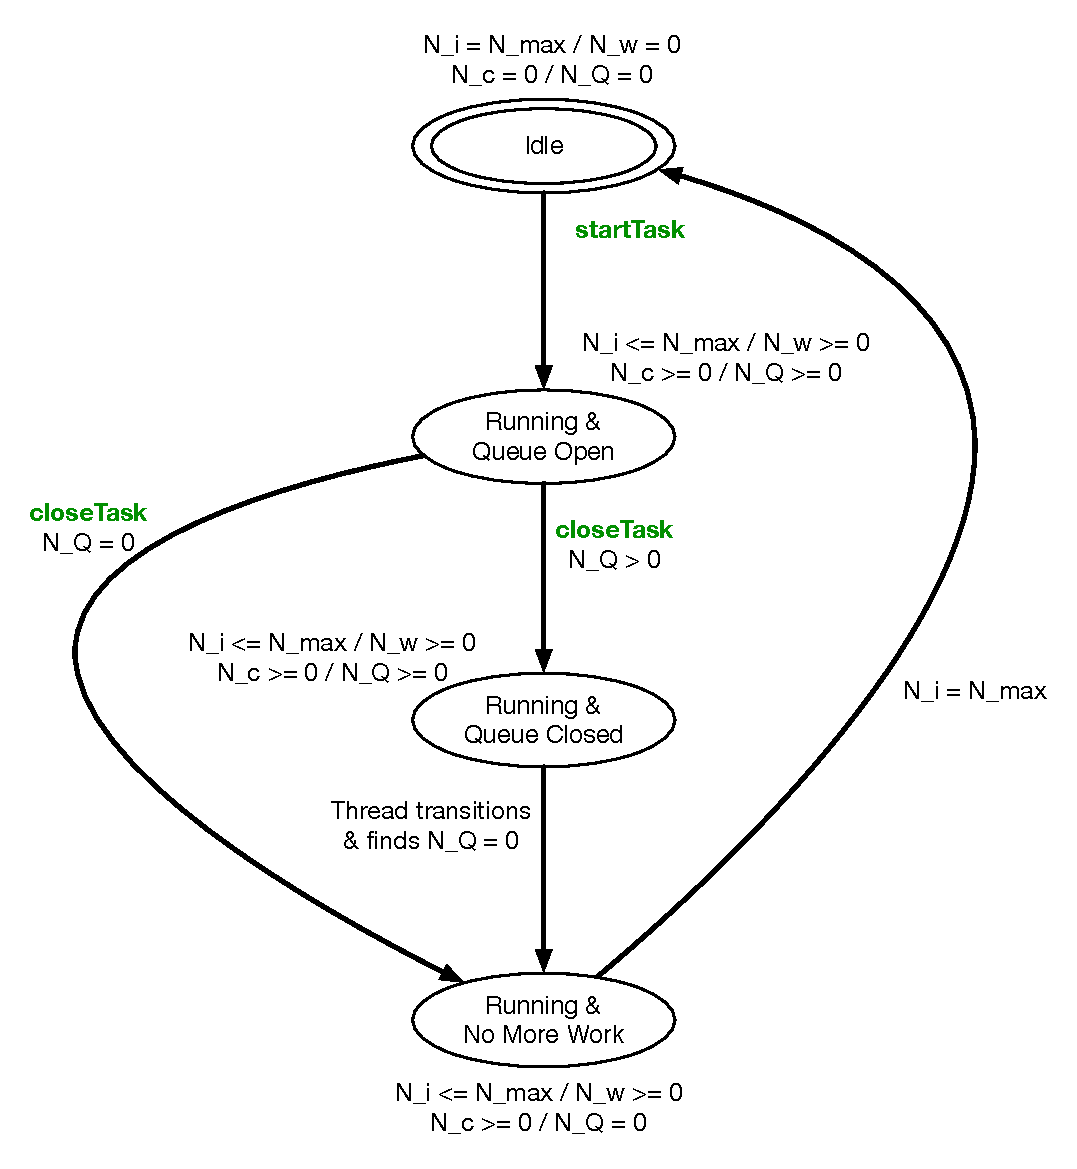
\includegraphics[width=5.0in]{TeamStates.pdf}
\caption[]{}
\label{fig:TeamStateDiagram}
\end{center}
\end{figure}

\begin{figure}[!hp]
\begin{center}
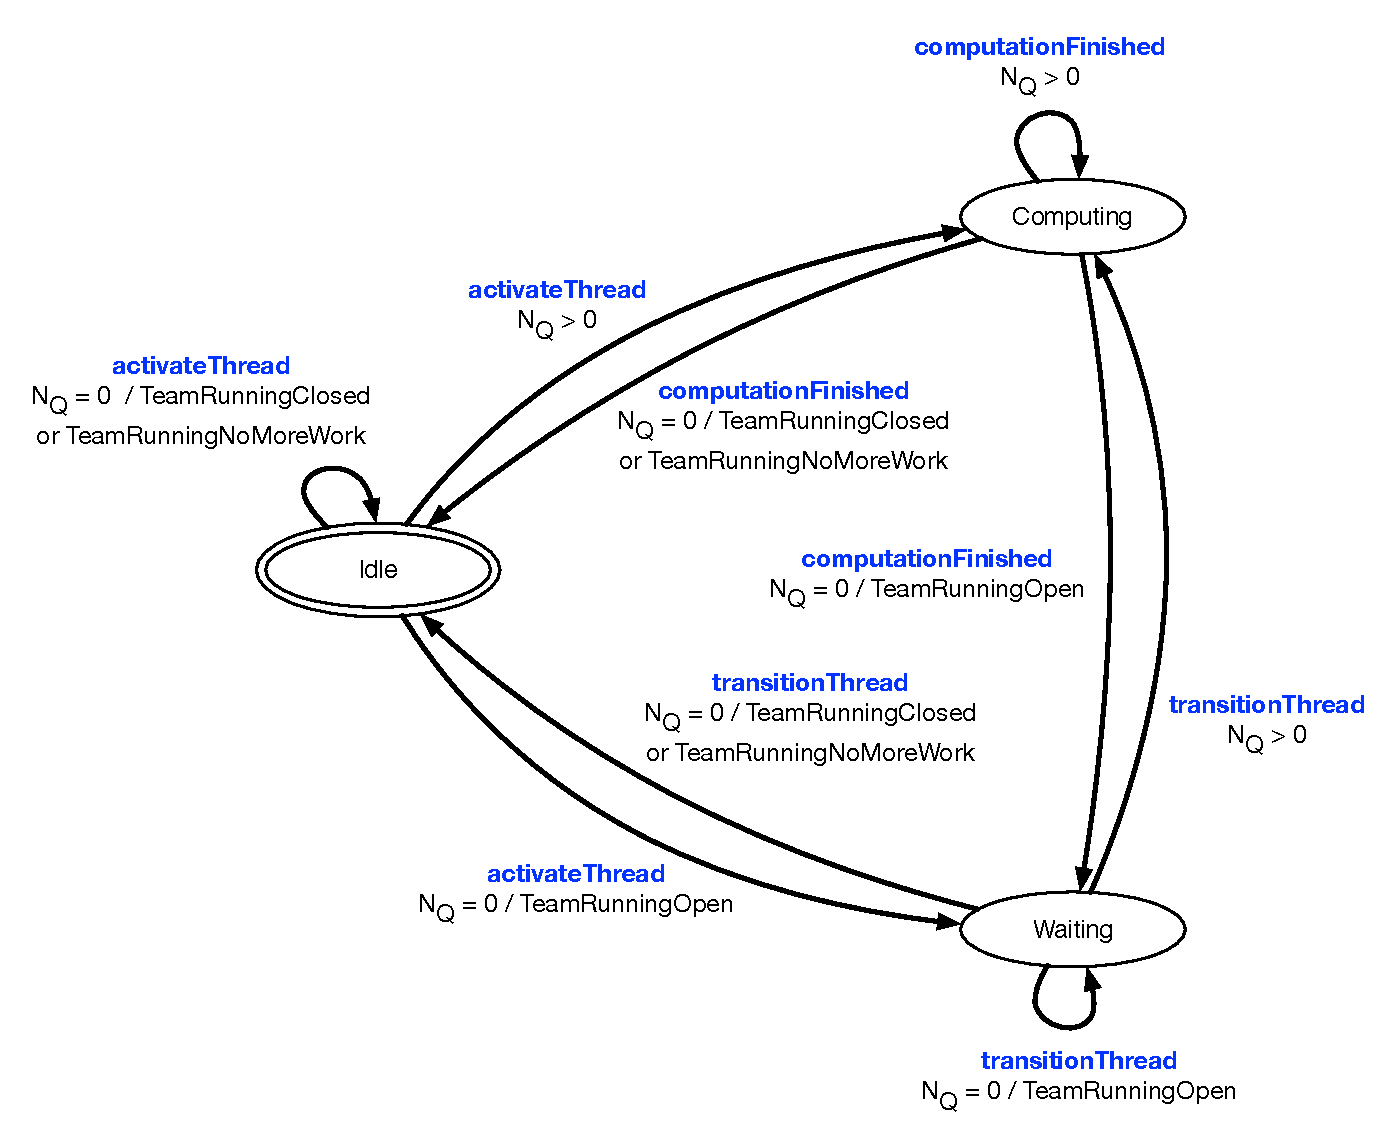
\includegraphics[width=6.5in]{ThreadStatesPersistent.pdf}
\caption[]{}
\label{fig:ThreadStateDiagram}
\end{center}
\end{figure}


\begin{spec}
\label{spec:Runtime_AtomicTransition}
As per the requirements of FSMs, each transition shall be implemented so that
the code executing the transition has sole access to the thread team's state,
during the entirety of the transition.  This implies that no other thread can
alter the state simultaneously, and that transitions are atomic.
\end{spec}
\textbf{Verification:}\hspace{0.125in}  Each thread team has a single,
dedicated mutex that must be acquired to access or alter thread team state
information.  Each transition acquires the mutex either through an explicit
request, or by a thread receiving an event.  The mutex is not released until
the transition is finalized.\\


Given the present implementation, it is important for transitions that
change the mode and emit internal signals, that the code change the mode
\textbf{first}, and then emit the signals.  This prevents the possible
(\textbf{TBC} for pthreads?) case that the signal is emitted and received before
the mode is correctly transitioned, which would violate
Spec~\ref{spec:Runtime_AtomicTransition}, and cause the responding thread
to react to the signal is a way that is potentially not in accord with the true
mode of the EFSM.

\begin{spec}
A thread team shall maintain a set of pending units of work, and all threads in a
thread team shall be able to check the set of pending units of work.  In
addition, each thread in the team shall be able to claim ownership of a single
unit of work by removing it from the set, with the understanding that the thread
itself is responsible for applying the team's \taskroutine to that unit of work.  It
shall be impossible for two threads to simultaneously claim ownership of the
same unit of work.
\end{spec}
\textbf{Verification:}\hspace{0.125in}  Pending work queues implemented as
stated.  As per Spec~\ref{spec:Runtime_AtomicTransition}, dequeueing of units of
work are only done after obtaining the mutex and no handle to dequeued units of
work remain.  Therefore, the only thread that can access a dequeued unit of work
is the thread that dequeued it.
\begin{spec}
All threads that transition to Idle must wait for the \texttt{activateThread}
event.  This includes threads in Idle that receive the \texttt{activateThread}
event but remain in Idle, as well as all threads that are \textit{set} into the
Idle state, when the EFSM is set up in the initial state.
\label{spec:IdleActivateThread}
\end{spec}

\begin{spec}
External code shall only be able to decrease $N_i$ through the
\texttt{startTask} and \texttt{increaseThreadCount} events, and the runtime shall
be implemented such that a request to activate $i$ threads results in an error
if $i$ exceeds the number of Idle threads that are available for activation.
Note that this technical specification is consistent with
Req~\ref{req:ThreadBalance}.
\end{spec}
\textbf{Verification:}\hspace{0.125in}  In the present design, this requirement
is important because the runtime would emit more \texttt{activateThread} signals
than there are threads to receive them.  Because teams allow for thread
publishers/subscribers, undetected signals would amount to a loss of thread
resources at the level of the runtime.  Note that a thread-based implementation
will have a lag between when these events trigger the activation of Idle threads,
and when these threads are actually activated.  The runtime design therefore
tracks the actual number of Idle threads with \texttt{N\_idle\_} = $N_i$, as well
as the number of threads pending activation with \texttt{N\_to\_activate\_}.
When a thread does receive \texttt{activateThread}, it decrements both
\texttt{N\_idle\_} and \texttt{N\_to\_activate\_} by one and increments by one
the internal state variable $N_i, N_w$ or $N_c$ corresponding to the thread's
next state.  To satisfy the requirement, both events throw an error if $i > $
\texttt{N\_idle\_} - \texttt{N\_to\_activate\_}.  No other public thread team
methods can emit \texttt{activateThread}.

\begin{spec}
\label{spec:Runtime_OneWait}
The interface of the thread team shall contain a \texttt{wait} method, so that
for each \taskroutine execution, the execution of an external thread that calls
\texttt{wait} is blocked until the termination of the \taskroutine.  This interface
shall allow for at most one such thread to block its execution with this method
during each \taskroutine execution.
\end{spec}
\textbf{Verification:}\hspace{0.125in}  Implemented a flag
\texttt{isWaitBlocking\_} to track if a thread has already called \texttt{wait}.

\begin{spec}
To maintain a simple design, client code shall only be allowed to attach and
detach thread subscribers when the team is in the {\TeamIdle} mode.  The same
requirement applies for work subscribers.
\end{spec}
\textbf{Verification:}\hspace{0.125in} Implemented directly as stated.

\begin{spec}
In the original designs, the Team state machine also contained a
{\TeamTerminating} mode.  The transition to this mode was allowed only from
{\TeamIdle}, and was triggered by initiating the destruction of the team.  While
sensible, this design was flawed since a runtime error that occurs with the team
in any state could trigger the destruction of the team.  Therefore, the
termination of the EFSM and the clean-up of its resources shall be possible from
any state.
\end{spec}
\textbf{Verification:}\hspace{0.125in}  The destructor does not do any error
checking to confirm that destruction was called with the EFSM in any particular
state.  Also, the destructor assumes that there are Idle, Waiting, and Computing
threads at the time of calling.  For the Idle and Waiting threads, it signals
them to terminate; Computing threads, it waits for them to finish their work and
discover that they should terminate.

\begin{spec}
\label{spec:Runtime_AwakenOnNoMoreWork}
All transitions to {\TeamRunningNoMoreWork} from a different mode shall awaken
all Waiting threads so that they can transition to Idle.
\end{spec}
\textbf{Verification:}\hspace{0.125in}  Implemented directly as stated.

\begin{spec}
\label{spec:Runtime_CompMustEnqueue}
Upon emitting/receiving the \texttt{computationFinished} signal, a Computing
thread shall enqueue the unit of work that it just finished applying the team's
\taskroutine to, with the team's work subscriber, if the team has a work subscriber.
\end{spec}
\textbf{Verification:}\hspace{0.125in}  Implemented directly as stated.

\begin{spec}
\label{spec:Runtime_IdleOutput}
All transitions to {\TeamIdle} from a different mode shall
\begin{itemize}
\item{call the \texttt{closeTask} method of the team's work subscriber (if it
has a work subscriber) and }
\item{unblock the external thread that called \texttt{wait}, if such a thread
exists.}
\end{itemize}
If the transition to {\TeamIdle} is handled by a Computing thread, then the
Computing thread shall enqueue its unit of work
(Spec~\ref{spec:Runtime_CompMustEnqueue}) prior to calling \texttt{closeTask}.
Note that this specification is not applicable to the case of \textit{setting}
the EFSM into its initial state.
\end{spec}
\textbf{Verification:}\hspace{0.125in}  Implemented directly as stated.

\begin{spec}
\label{spec:Runtime_IdleToIdle}
It is possible for an Idle thread to receive the \texttt{activateThread} event
when the team does not need threads to be activated (\textit{i.e.} the mode is
\TeamIdle \footnote{Consider a team that is both a thread publisher and
subscriber.  It is possible for the team to finish its work and transition to
{\TeamIdle} before its publisher and subscriber finish their work.} or
\TeamRunningNoMoreWork).  To avoid thread resource loss and to promote efficient
execution of the execution cycle's \taskroutines, in this scenario the threads that
receive the unnecessary event shall remain in Idle and call
\texttt{increaseThreadCount(1)} for its thread subscriber if it exists.
\end{spec}
\textbf{Verification:}\hspace{0.125in} Implemented directly as stated.

\begin{spec}
\label{spec:Runtime_ForwardThreads}
To prevent thread resource loss at the level of the runtime, all threads that
transition to Idle shall call \texttt{increaseThreadCount(1)} of its thread
subscriber, should it exist.  This specification is consistent with
Spec~\ref{spec:Runtime_IdleToIdle}, which could be understood to handle the
special case that an Idle thread transitions to Idle.  Note that this
specification is not applicable to the case of \textit{setting} the EFSM into
its initial state. This technical specification is consistent with
Req~\ref{req:ThreadSubPub}.
\end{spec}
\textbf{Verification:}\hspace{0.125in} Implemented directly as stated.

\begin{spec}
\label{spec:Runtime_NoEnqueue}
Client code shall only be allowed to give a team a unit of work if the team is
in the mode {\TeamRunningOpen}.  While the runtime could allow clients to give
units of work to a team that is in {\TeamIdle}, with the understanding that the
work would be for the next \taskroutine to be given to the team, there is no known use
case for which this is necessary.  Thus, this specification is motivated by
the goal of simplifying the design.
\end{spec}
\textbf{Verification:}\hspace{0.125in}  The \texttt{enqueue} method is the only
means for giving a unit of work to a team.  Attempts to use this method when the
team is not in {\TeamRunningOpen} result in error.\\

Based on this specification, client code should call \texttt{startTask} on all
thread teams to be used on a \taskroutine before enqueueing work with any of these.  This
practice will help avoid the case where an active work publisher tries to
enqueue work on a work subscriber that is still in the mode \TeamIdle.\\

As a final note, the design accounts for \texttt{transitionThread} events that
occur when no Waiting threads exist.  For each of these, this occurrence is
acceptable, and no output is generated as part of the transition.  This
transition is included for the sake of completeness and can occur with the
current implementation when certain outputs broadcast \texttt{transitionThread}.
Unlike for \texttt{activateThread}, it is unimportant that there is no thread to
receive the event.  This is due to the fact that this event exists to inform a
Waiting thread to look for work or that it should determine that it should
transition to Idle.  If there are no Waiting threads because all threads are
Idle, then the team must be in \TeamIdle, (in which case we don't need to
activate threads,) or in \TeamRunningOpen.  In \TeamRunningOpen we wait for
threads to be activated or for \texttt{closeTask} to be called to transition
the team to \TeamIdle.  If all threads are Computing, then these will discover
that there is pending work and the team will stay maximally busy.

%%-- TEAM IDLE SUBSECTION
\subsubsection{{\TeamIdle} State}
\begin{spec}
Similar to Spec~\ref{spec:Runtime_ForwardThreads}, if client code calls the
\texttt{increaseThreadCount} method of a thread team in \TeamIdle, the team shall
forward the pushed thread resources immediately on to its thread subscriber if
it exists.
\end{spec}
\textbf{Verification:}\hspace{0.125in}  Implemented directly as stated.

\begin{spec}
In the {\TeamIdle} mode, the queue shall always be empty, with all threads in the
team in the Idle state.  This implies that no thread can be in the Waiting
state, the Computing state, or terminating, and that all threads are
(Spec~\ref{spec:IdleActivateThread}) waiting to receive the
\texttt{activateThread} event.
\end{spec}
\textbf{Verification:}\hspace{0.125in}  The initial state starts in {\TeamIdle},
and specifies that there is no work in the queue.  Also, all transitions to
{\TeamIdle} only happen if the queue is empty.  Therefore, the pending work
queue is always empty upon entry to \TeamIdle.  Finally, no work can be added to
the queue in the {\TeamIdle} state by Spec~\ref{spec:Runtime_NoEnqueue}.\\

The initial state specifies that all threads are Idle, and transitions to
{\TeamIdle} only happen if the same is true.  Therefore, the claim is true upon
entry to {\TeamIdle}, and all threads are waiting for \texttt{activateThread}.
Responses
\footnote{These cases are being considered if one of these
events be emitted when the team in not Idle, but is received after transitioning
to Idle.  With the current implementation, since all threads would be waiting on
\texttt{activateThread}, no threads would be waiting for the latter two events.}
to \texttt{activateThread}, \texttt{transitionThread}, and
\texttt{computationFinishes} do not transition the thread state and have the
responding threads wait for \texttt{activateThread}.  Any attempt to
transition a thread terminates with the thread in Idle.

\begin{spec}
It would seem to be sensible to insist that an external thread cannot call
\texttt{wait} for a team that is in \TeamIdle.  However, it is possible that a
runtime execution cycle could finish and transition a team back to {\TeamIdle},
before an external thread has the chance to call \texttt{wait}.  Therefore, the
\texttt{wait} method shall be enabled in {\TeamIdle} and shall terminate immediately to avoid
unnecessary blocking of the calling thread.  This does allow for
client code to superfluously call \texttt{wait} before the first execution cycle
is run and multiple times between cycles, both of which are logical errors.
\end{spec}
\textbf{Verification:}\hspace{0.125in}  Implemented directly as stated and in
accord with Spec~\ref{spec:Runtime_OneWait}.

%%-- TEAM RUNNING & OPEN SUBSECTION
\subsubsection{\TeamRunningOpen}
\begin{spec}
It would seem sensible to insist that an external thread cannot call
\texttt{wait} during a given execution cycle, unless the \texttt{closeTask} event
has already been issued for the same cycle.  Consider the case of two
team one of which is the work publisher for the other.  As per
Spec~\ref{spec:Runtime_IdleOutput}, when the publisher team transitions to
{\TeamIdle}, it calls the subscriber's \texttt{closeTask} method to inform the
subscriber that it will not be given more work.  This implies that the external
thread that triggers an execution cycle with the runtime does not know when
\texttt{closeTask} is called, and could call \texttt{wait} before this
event occurs.  Hence, a thread team in the state {\TeamRunningOpen} shall allow
for a thread to call \texttt{wait}.
\end{spec}
\textbf{Verification:}\hspace{0.125in}  Implemented directly as stated.

%%-- TEAM RUNNING & CLOSED SUBSECTION
\subsubsection{\TeamRunningClosed}
\begin{spec}
\label{spec:Closed_Transition}
If a team is in mode \TeamRunningClosed, then every thread that transitions to
Computing shall check if $N_Q = 0$ as part of the transition, and after
dequeueing the unit of work on which it will apply its team's \taskroutine.  If $N_Q =
0$, then during the same transition (and therefore before applying the \taskroutine to
the dequeued unit of work) the thread shall change the mode to
\TeamRunningNoMoreWork.
\end{spec}
\textbf{Verification:}\hspace{0.125in}  A thread can be transitioned to
Computing from the Idle, Waiting, and Computing state.  If the mode is
{\TeamRunningClosed}, $N_Q = 1$, and a
thread receives any of the \texttt{activateThread}, \texttt{transitionThread},
or \texttt{computationFinished} events, then the induced transitions always changes
the mode to \TeamRunningNoMoreWork.  No other events result in decreasing $N_Q$
to zero in \TeamRunningClosed.

\begin{spec}
\label{spec:Closed_NoWork}
The transition from {\TeamRunningClosed} to \TeamRunningNoMoreWork (which is the
only transition possible for this mode,) is triggered internally by the active
thread that dequeues the last unit of work (Spec~\ref{spec:Closed_Transition}).
To avoid deadlock, the design of the runtime shall be such that the
EFSM cannot be in mode {\TeamRunningClosed} with $N_Q = 0$.  It is not
necessarily an error if $N_i = N_{max}$ in {\TeamRunningClosed}, as the team
could be a thread subscriber and have a thread activated by its publisher, so
that the team could eventually dequeue elements and determine that there is no
more work.
\end{spec}
\textbf{Verification:}\hspace{0.125in}  The only transition to
{\TeamRunningClosed} is from {\TeamRunningOpen}, which only occurs if $N_Q > 0$.
Hence, the specification is satisfied upon entry into the mode.  The value of
$N_Q$ can decrease in this mode only when a thread transitions to the Computing
state.   By Spec~\ref{spec:Closed_Transition}, the EFSM mode is transitioned to
{\TeamRunningNoMoreWork} as part of every transition that results in $N_Q = 0$.

%%-- TEAM RUNNING & NO MORE WORK SUBSECTION
\subsubsection{\TeamRunningNoMoreWork}
The only transitions into {\TeamRunningNoMoreWork}
are from {\TeamRunningOpen} and \TeamRunningClosed.

\begin{spec}
\label{spec:NoMoreWork_NoWork}
If a team is in \TeamRunningNoMoreWork, then it shall always be true that $N_Q =
0$.
\end{spec}
\textbf{Verification:}\hspace{0.125in}
Since both methods of transition into {\TeamRunningNoMoreWork} only occur if $N_Q = 0$,
the specification is satisfied upon entry to the mode.  The only means to
increase $N_Q$ is by adding work \textit{via} \texttt{enqueue}, which is
prohibited in {\TeamRunningNoMoreWork} by Spec~\ref{spec:Runtime_NoEnqueue}.

\begin{spec}
\label{spec:NoMoreWork_TransitionToIdle}
If a team is in mode \TeamRunningNoMoreWork, then the last thread to transition
to Idle shall change the mode to \TeamIdle.  This transition is valid as $N_i =
N_{max}$ necessarily at the transition and by Spec~\ref{spec:NoMoreWork_NoWork}
it is certain that $N_Q = 0$.
\end{spec}
\textbf{Verification:}\hspace{0.125in}  If the transition to
{\TeamRunningNoMoreWork} is from \TeamRunningOpen, then $N_w > 0$ or $N_c > 0$
(to the contrary, $N_Q = 0$ and $N_i = N_{max}$ so that the transition is to
\TeamIdle).  If the transition is from \TeamRunningClosed, then it follows from
Spec~\ref{spec:Closed_Transition} that $N_c > 0$.  Therefore, upon entry to the
mode, there is at least one thread that could transition to Idle.  Since
satisfaction of Spec~\ref{spec:NoMoreWork_NoWork} implies that $N_Q = 0$, all
Computing threads will determine that there is no more work
upon finishing the application of the team's
\taskroutine to the current unit of work, and threads will
subsequently transition to Idle.  Similarly, satisfaction of
Spec~\ref{spec:Runtime_AwakenOnNoMoreWork} implies that all threads in the Wait
state will be awakened, determine that there is no work, and transition to Idle
as well.  All non-active threads will eventually transition to Idle.
Given this and the fact that the reception of \texttt{activateThread} events are
effectively ignored by Idle threads, we conclude that there will be a last
thread that transitions to Idle.  This thread is programmed to transition the
mode to \TeamIdle.

\begin{spec}
\label{spec:NoMoreWork_NeedThread}
The transition from {\TeamRunningNoMoreWork} to \TeamIdle, which is the only
transition out of this mode, occurs when the last non-Idle thread transitions to
Idle (See Spec~\ref{spec:NoMoreWork_TransitionToIdle}).  Therefore, to avoid
deadlock the design of the runtime shall prohibit the EFSM from being in a state
with {\TeamRunningNoMoreWork} and $N_i = N_{max}$.
\end{spec}
\textbf{Verification:}\hspace{0.125in} As shown in the Verification of
Spec~\ref{spec:NoMoreWork_TransitionToIdle},  $N_i < N_{max}$ upon entry to the
mode. $N_i$ can only decrease by at most one with each thread transition,
which are atomic (Spec~\ref{spec:Runtime_AtomicTransition}). Satisfaction of
Spec~\ref{spec:NoMoreWork_TransitionToIdle} implies that $N_i$ cannot be set to
zero in {\TeamRunningNoMoreWork} without also simultaneously causing the mode to
change to \TeamIdle.  Hence, $N_i < N_{max}$ in {\TeamRunningNoMoreWork} up to
the transition to \TeamIdle.

%%-- DATA PACKET SUBSECTION
\subsubsection{Data Packets}

One of the main difficulties associated with running software on host-device
nodes is the runtime penalty incurred by moving data between the host memory and
remote device memory.  This difficulty influences heavily the
high-level design of the orchestration system and the runtime.  It is
important enough that it influences the design decisions made within the
lower-levels of the software design and implementation.  The concept of a data
packet, and the ability of thread teams to have data packet of tiles as its data
type, is one of the fundamental aspects for addressing this difficulty.
The data packet is introduced to allow
the runtime to asynchronously shuttle data between the host and device in a
pipelined format, where the user can specify the size of each data packet that
will flow through the pipeline.  The user will be able to fine tune
the size of the data packets, so that they are small enough that the use of the
pipeline is merited and to achieve good latency hiding, but large enough that
the devices will always have enough work once the pipeline is wound up.\\

Since the data packet contains tiles, it must also provide device code with
associated tile metadata.  This could mean that the data packet includes
the tile metadata, pointers to the
metadata in the device memory, or a unique tile index for retrieving all
metadata.  It seems that the data packet could be a generalization of
\code{Grid\_tile\_t}.  A data packet of one tile, while perhaps overly
heavy, is a possibility.\\

Ideally, the data packets will be the heaviest and sole users of the runtime
memory management services.  Rather than dynamically allocating
all memory for the data packet in special host memory (\eg pinned memory) and in
device memory (which would be very inefficient), the data packets will acquire
their memory by requesting resources from the memory manager's memory pools.\\

Given that each data packet owns memory resources that are acquired at creation
and that no part of the code owns a data packet (since these are passed around),
the implementation of the flow of data packets within the runtime operational
environment must be designed carefully. The element in the thread team
configuration that is the final consumer of a data packet must ensure that the
resources owned by the data packet are released properly.

\begin{spec}
Each class that implements a data packet shall provide a public member function
that releases all resources owned and managed by a data packet object.  Program
flow shall continue unimpeded if this member function
is called before the data packet requests or allocates such resources.
\end{spec}

\begin{spec}
Data packets shall only be created, packed, and unpacked by the runtime or by
code written by the Orchestration System's offline toolchain.  This implies that
static Fortran code shall never be exposed to a data packet nor know that data
packets exist.  This is sensible as one tentative defining characteristic of
such a routine is that it works on a per-tile basis.
\end{spec}

\begin{spec}
Since tile objects can be passed around the code as part of the contents of a
data packet, the ownership of each tile object shall be taken over by a data
packet when the tile is added to the data packet.  For each
tile there may be several tile objects simultaneously in existence.  One tile
object might be flowing through a CPU concurrent pipeline in
the thread team configuration, while a second copy has been included in a data
packet that is flowing through the concurrent GPU pipeline.  This implies that
if tile objects associated with the same tile have a shared resource that must
be released, then the resource must only be released once the last of the tile
objects is no longer needed.  In the interest of simplicity, no tile
object shall own resources that will require explicit release by the runtime, and
the data packet need not include any functionality to manage tile-specific
resources.
\end{spec}

\begin{spec}
The data packet interface shall include a public routine that allows client code
to add a given tile object to the data packet.  For full flexibility
and runtime efficiency, this routine shall allow copying the given tile
object into internal data packet data structures or moving the given tile object
information into the data structures.  It is the responsibility of the calling
code to indicate if a copy or a move shall be used.
\end{spec}

Some data items may be allocated dynamically, and therefore require deallocation,
once they have been used by the thread team configuration.  Some data items
might own resources that need to be released.  There might be some
data items that fit both descriptions.  Such data items flow through
a thread team configuration. The management of the ownership of these must be
done carefully so that all associated resources are released appropriately.

% Thread team configuration section
\begin{spec}
A thread team configuration shall consist of an action parallel distributor,
which enqueues each data item provided by an iterator constructed from a given
iterator specification, and one or more action parallel pipelines.  Two
pipelines are action parallel pipelines if data items are not passed between the
pipelines, and each routine to be applied in one pipeline is pairwise independent
of all routines to be applied in the other pipeline.
\end{spec}

Claim: An action parallel pipeline will apply its constituent actions to each
data item, given to the distributor by its iterator.

Claim: For a given data item, the ordering of which routine is applied to the
item within a pipeline is important and maintained.  The order of which
routine is applied to the item across pipelines is unimportant.

\begin{spec}
When a data item is enqueued with a thread team, it shall be made clear in the
design and implementation that the thread team assumes ownership of the item.
If a thread team does not have a work subscriber, then ownership of the data
item terminates when a thread in the team finishes applying the team's assigned
action to the item.  If a thread team has one or more work subscribers, then
ownership of the data item is transferred to the work subscribers on an
individual basis when enqueued with the subscribers.  Thread teams shall not
create or destroy data packets. All thread teams whose data type is
a data packet shall have a work subscriber so that there will exist, in the
thread team configuration, a downstream entity that will manage the destruction
of the data packet.
\end{spec}
Data packets shall be created only by distributors and data item aggregators.

\begin{spec}
A data packet shall allow for the sharing of data defined on tiles as well as the
sharing of non-tile-based data in the form of scalars, arrays, structs, and classes.

\end{spec}


\begin{figure}[!hp]
\begin{center}
\includegraphics[width=5.0in]{DataPacket_CpuGpu.pdf}
\caption[]{An example of a data packet  for the
GPU-concurrent/Post-gpu pipeline in Figure~\ref{fig:ConcurrentItor}.  The
leftmost graphic is the total data packet, and the rightmost graphics are zooms
of individual structures that are included in the data packet for each tile
contained in the packet.  Each
colored block corresponds to one particular object.  Each object to be included
 in the data packet is classified as either copyin,
copyinout, or copyout. Copyin means to be copied from host to device only,
copyout is from device-to-host only, and copyinout is from host-to-device-to-host.
The different objects have been located within the data packet based on this
classification, and allow transfers to be executed as a transfer of one
contiguous block of memory, only transferring the necessary data.  The arrows
and associated text
on the rightside of the data packet indicate pointers that can be used to find
inidividual subsections of the data packet.  The green tile metadata elements
could be the actual metadata itself or device pointers to metadata cached in
device memory.  The gray blocks are the actual tile data. The blue blocks
hold device pointers to the start of the associated grey blocks in device
memory.}
\label{fig:DataPacket_CpuGpu}
\end{center}
\end{figure}

\newpage
\begin{appendices}
\section{A Menagerie of Configurations}
\label{adx:ConfigMenagerie}

Possible thread team configurations have been presented and
motivated in Section~\ref{sec:Definitions}.  While these examples help to
understand the basic design of the runtime, they also serve as use cases and
assist to inform the design.  This section presents a menagerie of
thread team configurations.  Where possible,
each configuration is accompanied by a hypothetical motivating example.  Since
it is simple to scale up thread team configuration in size by adding
one or more teams, we choose to only include in the menagerie those
examples that introduce new complexity, and capture the complexity with the
smallest possible size.\\

To make this collection more useful, all of the
configurations in the collection will be used by a single simulation.  To allow
for this, the simulation must instantiate
\begin{itemize}
\item{thread team 1 with data type Tile,}
\item{thread team 2 with data type Data Packet of Blocks,}
\item{thread team 3 with data type Tile,}
\item{thread team 4 with data type Action Metadata,}
\item{thread team 5 with data type Data Packet of Blocks,}
\item{thread team 6 with data type Data Packet of Tiles,}
\end{itemize}
which is the minimal set of thread teams necessary to create all of the thread
team configurations when only one configuration can exist at a time.  In
addition, we are assuming that each MPI rank will be assigned to run on 4 cores
with 2 hardware threads each (8 processing elements/rank).  We further assume we can
oversubscribe these resources with 10 threads, so long as only a small number of
those threads are executing heavy computation during an orchestration runtime
execution cycle.\\

The examples are presented in order of increasing complexity.  The number of details
 in the captions decrease, with the understanding that the
reader will be able to determine which details in earlier examples apply to the
later examples.  The intent is that these be read in order.

\begin{figure}[!ht]
\begin{center}
\includegraphics[width=3.0in]{CpuOnlyConfiguration.pdf}
\caption[]{The hello world of thread team configurations.  Indeed Action A could
be to print ``Hello, world, from tile $i$'' for each tile enqueued with Team 1.
In this case, the processing elements will all be used for ``heavy''
computation, and to achieve runtime efficiency,
the thread team must use fewer threads than the total number of processing
elements.  While the distributor being used is an action parallel distributor,
it is the trivial action parallel distributor, since there is only a single
action being applied by this configuration.  Any computation that needs to be
carried out on all blocks in the domain is a motivating example for this simple
configuration.  The computation needed to apply action A should be
sufficiently heavy that the overhead of the thread team is overcome.}
\label{fig:CpuOnlyConfig}
\end{center}
\end{figure}

\begin{figure}[!ht]
\begin{center}
\includegraphics[width=5.0in]{GpuOnlyConfiguration.pdf}
\caption[]{This configuration is the simplest, realistic thread team
configuration that would be used to apply an action using a device with
dedicated remote memory (\eg a GPU).  In this case, a trivial action parallel
distributor will group blocks into data packets and transfer these
asynchronously to the device memory.  Specifically, the distributor will
aggregrate blocks in a single data packet, until it is sufficiently large.  The
distributor then copies the data packet from host to GPU memory and
enqueues the data packet with Team 2.  A thread in Team 2 can begin
applying Action B, to blocks in the data packet, at the same time that the
distributor can begin forming the next data packet.  Once the first
data packet is sent, the runtime overlays data movements and computation to
achieve latency hiding.  When a thread in Team 2 has finished applying action B
to all blocks in its current data packet, it will enqueue the data packet of
blocks with the data mover (DM) and unpacking work subscriber.  This, in turn,
will asynchronously transfer the data packet back to host memory, move
data from the host-side data packet to its appropriate location in the Grid unit's data structures, and
release the data packet's resources.  We do not
leave the data in the remote device memory, as we do not want to assume that the
total amount of data needed to apply the action to all blocks managed by the
runtime's MPI rank (including the block data) can fit in the remote memory.  As
no host processing elements will be used for heavy computation, we can
oversubscribe the host processing elements with a large number of orchestration
threads.  Any computation, that needs to be carried out on all blocks in the the
domain, is a motivating example for this simple configuration.  Due to
the overheads of the thread team, packing/unpacking the data packet, and the two
data transfers (latency and transfer), the runtime of the kernels should be
large (\textbf{TBC}).  It is possible (\textbf{TBC}) that
the kernel runtimes could be smaller, so long as the number of data packets sent
down the pipeline is sufficiently large.}
\label{fig:GpuOnlyConfig}
\end{center}
\end{figure}

\begin{figure}[!hp]
\begin{center}
\includegraphics[width=3.0in]{GpuInternalConfiguration.pdf}
\caption[]{We show an unusual use case that avoids requiring data packets for applying
actions using a device with dedicated remote memory.  A hypothetical motivating case
would be an operation
that works with cached non-Grid-owned data, that is only used by kernels run in
the GPU.  We could imagine that the data is allocated and
initialized when the simulation starts, and with each time step the data is
corrected by Action B.  In order for this action to run correctly, it would need
the host to inform kernels what data should be used to determine the
correction, as well as a device pointer to the location of the cached data (\ie
Action Metadata).  In a directive-based implementation of action routine B, these
parameters would be extracted from the given Action Metadata item and these used
in GPU offload directives.
\label{fig:GpuInternalConfig}
\end{center}
\end{figure}

\begin{figure}[!hp]
\begin{center}
\includegraphics[width=4.25in]{CpuGpuActionParallel.pdf}
\caption[]{This configuration consists of two parallel pipelines. One
pipeline is executing an action routine that uses only the host to apply Action A
to all tiles being managed by the runtime's MPI rank. The other is executing an
action routine that applies to the same data, Action B using a GPU.  This example
demonstrates the true nature of an action parallel distributor --- it feeds all
the tiles in the appropriate data type to each of the pipelines.  For this
configuration to always apply the actions correctly, it must be the case that
Action A and Action B can be run independently (\ie they do not have any data
dependencies).  As in Figure~\ref{fig:GpuOnlyConfig}, the configuration uses
data packets and a data mover for the pipeline that uses a GPU.  We think
 it is best to give more threads to the thread team that
launches kernels on the GPU, so that the orchestration threads in
Team 2 can continuously feed the GPU with enough data that the GPU will be
maintained at maximum occupancy.  This configuration could be easily
scaled up in terms of the number of pipelines being fed by the action parallel
distributor.  For instance, the distributor could feed a third thread team that
would apply some Action C using an FPGA so long as actions A, B, and C do not
have any pairwise data dependencies.}
\label{fig:CpuGpuActionPConfig}
\end{center}
\end{figure}

\begin{figure}[!hp]
\begin{center}
\includegraphics[width=5.5in]{CpuGpuDataParallel.pdf}
\caption[]{A data parallel version of Figure~\ref{fig:CpuGpuActionPConfig}.  In
this case, we choose to use host and device resources to efficiently apply only
Action A in a single runtime execution cycle by splitting the data between CPU-
and GPU-based pipelines.  Specifically, the data parallel distributor will be
equipped with an algorithm that determines whether a block should be decomposed
into tiles and enqueued with Team 1, or added to a data packet that will
eventually be shipped to the GPU and enqueued with Team 2.  Once a
runtime execution cycle has completed, Action A will have been applied to all
tiles that the runtime's MPI rank is managing.  This configuration also
could be easily scaled up in terms of the number of pipelines being fed by the
data parallel distributor.  For instance, we could have a third team added to
the configuration that will apply Action A using an FPGA, and extend the data
parallel distributor to partition the full set of tiles across the three thread
teams.}
\label{fig:CpuGpuDataPConfig}
\end{center}
\end{figure}

\begin{figure}[!hp]
\begin{center}
\includegraphics[width=4.5in]{HybridDistributorExample.pdf}
\caption[]{This configuration example is a simple, interesting extension of
the configurations in Figures~\ref{fig:CpuGpuActionPConfig}
and~\ref{fig:CpuGpuDataPConfig}.  The added complexity is that two of the three
pipelines function in a data parallel fashion to apply Action A, using both CPU
and GPU resources. The final pipeline is run in action parallel fashion
with respect to the Action A pipelines and using FPGA resources.   This setup
requries a hybrid distributor.  A related example would be for Action B to be
run on the same GPU as Action A or on a different GPU.  Note that Action A and
Action B should be data independent.}
\label{fig:HybridDistributorExample}
\end{center}
\end{figure}

\begin{figure}[!hp]
\begin{center}
\includegraphics[width=6.0in]{DataParallelWithAccumulator.pdf}
\caption[]{This configuration is an extension of the configuration in
Figure~\ref{fig:CpuGpuDataPConfig} with increased complexity by extending
and merging the two Action A pipelines through the addition of a third thread
team ,that applies Action B to all tiles managed by the runtime's MPI rank.
After the runtime execution cycle
terminates, Action B will have been applied to all tiles managed by the
runtime's MPI rank, but only after the application of Action A using either the CPU
or the GPU.  If Action A and Action B were data independent, then the
configuration in Figure~\ref{fig:HybridDistributorExample}
could have been used.  It is possible that there may exist data
dependencies requiring that
Action A be run before Action B.  This configuration is
also an extension of the configuration in Figure~\ref{fig:SplitItor}, as Action B
is applied by a device, rather than the host.  This twist necessitates a work
subscriber/publisher entity that accumulates tiles from Team 1, aggregates these
into data packet of associated blocks, and ships the data packets from the
host to the FPGA remote memory.  For this to work, if a tile is enqueued with
Team 1, then all other tiles in this tile's block must also be enqueued with
Team 1.  An interesting tweak to this configuration would be to have Team 5
apply Action B using a second GPU, in which case the associated data mover would
affect an inter-GPU data movement.}
\label{fig:DataPWithAcc}
\end{center}
\end{figure}

\begin{figure}[!hp]
\begin{center}
\includegraphics[width=6.0in]{HybridDistributorExample2.pdf}
\caption[]{A conglomeration of the configurations in
Figures~\ref{fig:HybridDistributorExample} and~\ref{fig:DataPWithAcc}. Work
publisher/subscriber connections are used to construct piplines in a
thread team configuration.  Thread publisher/subscriber connections are
not restricted whatsoever by the structure of a configuration, nor do they affect
the structure in any significant way.  Rather, these connections are something
close to a decorator added to a configuration to aid in load
balancing.  For this configuration, Team 6 is a thread publisher for a
team in a different pipeline.}
\label{fig:HybridDistConfig2}
\end{center}
\end{figure}

%\begin{figure}[!hp]
%\begin{center}
%\includegraphics[width=5.0in]{}
%\caption[]{}
%\label{fig:}
%\end{center}
%\end{figure}

\end{appendices}
%\subsection{Possible Requirements}
%If a thread team is going to ship data to an accelerator like a GPU, then the
%unit of work for such a thread team shall be a data packet of tiles (with the
%possibility that the tiles are the trivial tiling).  This includes the
%possibility of data packets that consist of a single tile (and therefore tile
%that consist of a single block).

%If a thread team is going to ship data to the host, then the unit of work for
%such a thread team shall be a tile (with the possibility that the tiles are the
%trivial tiling).

%Consider a unit of runtime work that includes a GPU-concurrent \taskroutine, a
%CPU-concurrent \taskroutine, and a Post-concurrency CPU \taskroutine in its \actionroutinebundle.  Then
%for each block in a data packet, the concurrent CPU \taskroutine will have blocks of
%input data (CC, FC[XYZ], Fluxes[XYZ], etc.), output data (CC, FC[XYZ],
%Fluxes[XYZ], etc.), and scratch blocks (e.g. grav[XYZ], auxC).  The concurrent
%GPU \taskroutine will have the same, but non-intersecting block structure.  The
%post-concurrency CPU \taskroutine can use whatever is in MFabs that is not being worked
%on by the concurrent CPU \taskroutine and can allocate its own CPU scratch blocks.  We
%can get the CPU scratch memory through the runtime memory manager, but I don't
%know if we need to manage that memory or just let failures happen.  This assumes
%that the host memory will never be the limiting memory pool factor (i.e. that
%the host memory will always be much larger than the device memory).\\

%It is possible that certain units of runtime work will not need to bring the
%data back to the host memory as that same data is needed by the next runtime
%execution in the same device.  However, since we cannot assume that all the
%memory will fit in the device memory, we must assume that in the worst case only
%a fraction of the intended blocks will stay in the device memory.  The runtime
%shall maintain location information for each block that persists across calls to
%the runtime.  When the next runtime execution begins, those blocks already in
%the device shall be grouped into one or more data packets and work immediately
%launched on these.  The runtime shall not include these same blocks in a
%subsequent data packet so that we avoid repeated work.  \FlashOfTheFuture shall abort
%execution if, at the end of a solution advance phase, we have blocks of persistent data
%(\textit{e.g.} unk) that are not in the host memory.  \Jared{Are these
%really requirements that we want?  If yes, then the blocks in the device memory
%would be the first data packet and therefore we get the pipeline up and running
%quicker.}  Example of this is unsplit Hydro.  The computeFluxes routine pulls in
%the UNK data on CC1 and updates the fluxes.  Neither needs to go back to the GPU
%ever.  The updated solution is in CC2.  Note that if we have the future case of
%host and some devices sharing the same physical memory, this requirement could
%become more imporatant.  Therefore, giving the runtime more parameters to inform
%data movements could be important.\\

%Should we allow the Post-concurrency \taskroutine to start immediately when blocks get
%back from the GPU?  This would imply that this \taskroutine is also independent from the
%CPU-concurrent \taskroutine.  Or, do we run the Post-concurrent \taskroutine only after both the
%CPU and GPU work have finished?  Note that we can never know that a single
%routine will always run on either the host or either the device.  They must be
%written in such a way that they can be run well on either without manual or
%automatically updating the code beyond directives (OpenACC, OpenMP, CUDA, etc.).\\

%\newpage
%\begin{appendices}
%\section{Hydro operations}
%The Unsplit implementation of the Hydro step operation has at least three
%variants and the variant executed at runtime is presently determined at each
%time step based on the Grid unit AMR implementation chosen (known at setup)
%and whether or not flux correction should be applied (specified as a runtime
%parameter).  Here we express each variant as an operation.\\
%
%\Jared{TODO: Add to requirements that parameter such as flux correction
%should be both a setup and runtime parameter.  If the setup-time value is false,
%then the task scheduler has the possibility to fuse \OLARs.  If it is true, then
%the runtime parameter can still be set to turn this off.  However, the binary
%built will not have been built with the potential for fusing \taskroutines.}\\
%
%For the following subsections, the colorization is
%\begin{itemize}
%\item{a \ComposerKey{keyword} that is paired with a static Fortran routine in
%the operation's dictionary,}
%\item{a \RuntimeParam{runtime} parameter, and}
%\item{a \SetuptimeParam{setup-time} and runtime parameter.}
%\end{itemize}
%
%TODO: Add in a UG variant?!
%
%\newpage
%\subsection{No flux correction variant}
%\texttt{
%\begin{tabbing}
%\hspace*{0.25in}\=\hspace*{0.25in}\= \kill
%if \SetuptimeParam{shockDetectOn}:\\
%\>\ComposerKey{GcFillWithoutEoS} (global, internode data movement)\\
%\> Task 1:\\
%\>\> \ComposerKey{doShockDetection}\\
%\ComposerKey{GcFillWithEoS} (global, internode data movement)\\
%Task 2:\\
%\> if \RuntimeParam{updateHydroFluxes}:\\
%\>\> \ComposerKey{updateHydroData}\\
%\> \ComposerKey{zeroFluxData}\\
%\> iterate \ComposerKey{LeavesWithoutTiling}:\\
%\>\> \ComposerKey{computeFluxesAndUpdateSolution}\\
%\end{tabbing}
%}
%
%For \ComposerKey{computeFluxesAndUpdateSolution}, the dictionary should know
%that it needs to run \texttt{hy\_computeFluxes} with \texttt{Uout => Uin}.
%
%\subsection{Paramesh + flux correction variant}
%\texttt{
%\begin{tabbing}
%\hspace*{0.25in}\=\hspace*{0.25in}\=\hspace*{0.25in}\= \kill
%if \SetuptimeParam{shockDetectOn}:\\
%\>\ComposerKey{GcFillWithoutEoS} (global, internode data movement)\\
%\> Task 1:\\
%\>\> \ComposerKey{doShockDetection}\\
%\ComposerKey{GcFillWithEoS} (global, internode data movement)\\
%Task 2:\\
%\> if \RuntimeParam{updateHydroFluxes}:\\
%\>\> \ComposerKey{updateHydroData}\\
%\> \ComposerKey{zeroFluxData}\\
%\> iterate \ComposerKey{LeavesWithoutTiling}:\\
%\>\> if level == finest:\\
%\>\>\> \ComposerKey{computeFluxesAndUpdateSolution}\\
%\>\> else:\\
%\>\>\> \ComposerKey{computeFluxes}\\
%\> \ComposerKey{storeFluxDataForFluxCorrect}\\
%\ComposerKey{conserveFluxes} (global, internode data movement)\\
%Task 3:\\
%\> iterate \ComposerKey{LeavesWithoutTiling}:\\
%\>\> if level == finest:\\
%\>\>\> \ComposerKey{noOp}\\
%\>\> else:\\
%\>\>\> \ComposerKey{updateSolution}\\
%\> \ComposerKey{updateBoundaries}
%\end{tabbing}
%}
%
%\newpage
%\subsection{AMReX + flux correction variant - tiling}
%\textbf{Input:} \texttt{simTime, dt, dtOld, sweepOrder}\\
%\textbf{Output:} the updated solution with EoS run on all leaf blocks.  GC data
%not necessarily good.
%
%\texttt{
%\begin{tabbing}
%\hspace*{0.25in}\=\hspace*{0.25in}\=\hspace*{0.25in}\=\hspace*{0.25in}\= \kill
%if \SetuptimeParam{shockDetectOn}:\\
%\>\ComposerKey{GcFillWithoutEoS} (global, internode data movement)\\
%\> Task 1:\\
%\>\> iterate \ComposerKey{LeavesOnLevelWithoutTiling}:\\
%\>\>\> \ComposerKey{doShockDetection} (operates on single block)\\
%\ComposerKey{GcFillWithEoS} (global, internode data movement)\\
%Task 2:\\
%\> if \RuntimeParam{updateHydroFluxes}:\\
%\>\> SubTask 2.1 (Run in device so that data is already in device memory?):\\
%\>\>\> \ComposerKey{updateHydroData} (doesn't operate on blocks, but sets
%variables)\\
%\> SubTask 2.2 (Run in CPU to avoid data movements?):\\
%\>\> \ComposerKey{zeroFluxData} (iterates over all leaf blocks)\\
%\ComposerKey{TaskBarrier} (fake data movement so that tasks are clean and efficient)\\
%Task 3:\\
%\> level = finest\\
%\> iterate \ComposerKey{LeavesOnLevelWithoutTiling}:\\
%\>\> \ComposerKey{computeFluxesAndUpdateSolution}\\
%\> if \ComposerKey{nLevels} > 1:\\
%\>\> \ComposerKey{storeFluxDataForFluxCorrect}\\
%\> level = finest-1 (NOTE: There might only be one level at any iteration!)\\
%\> iterate \ComposerKey{LeavesOnLevelWithoutTiling}:\\
%\>\> \ComposerKey{computeFluxes}\\
%\> if level != coarsest:\\
%\>\> \ComposerKey{storeFluxDataForFluxCorrect}\\
%\ComposerKey{conserveFluxes} (global, internode data movement)\\
%loop level=finest-1..coarsest:\\
%\>Task 3+i:\\
%\>\> iterate \ComposerKey{LeavesOnLevelWithoutTiling}:\\
%\>\>\> \ComposerKey{updateSolution}\\
%\>\> level = finest-i\\
%\>\> iterate \ComposerKey{LeavesOnLevelWithoutTiling}:\\
%\>\>\> \ComposerKey{computeFluxes}\\
%\>\> if level != coarsest:\\
%\>\>\> \ComposerKey{storeFluxDataForFluxCorrect}\\
%\ComposerKey{conserveFluxes} (global, internode data movement)\\[0.25in]
%Task M:\\
%if \SetuptimeParam{useGravity}:\\
%\> \ComposerKey{prepareNewGravityAccelerations}\\
%\ComposerKey{doGravityStep}
%\ComposerKey{TaskBarrier} (Implied because we are at the end of the operation?)
%\end{tabbing}
%}
%
%Note that \texttt{hy\_updateSolution} calls \texttt{hy\_energyFix} and \texttt{Eos\_wrapped}
%at the end.  These two could be pulled out and included as subtasks that could
%be run on the CPU after \texttt{hy\_updateSolution} finishes running on a data
%packet in the accelerator.\\
%
%Note that \texttt{hy\_prepareNewGravityAccelerations} can call
%Gravity\_potential and GcFill in the end.  This needs to be moved up.\\
%
%Note that \texttt{hy\_gravityStep} iterates over all leaf blocks to update the
%solution using the gravity accelerations.
%
%\end{appendices}

\end{document}
